% !TeX encoding = UTF-8

% 载入 SJTUThesis 模版
\documentclass[type=master]{sjtuthesis}
% 选项
%   type=[doctor|master|bachelor|course],     % 可选(默认:doctor),论文类型
%   zihao=[-4|5],                             % 可选(研究生默认:-4,本科默认:5),正文字号大小
%   lang=[zh|en],                             % 可选(默认:zh),论文的主要语言
%   review,                                   % 可选(默认:关闭),盲审模式
%   [twoside|oneside]                         % 可选(默认:twoside),单双页模式

% 论文基本配置,加载宏包等全局配置
% !TEX root = ./main.tex

\sjtusetup{
  %
  %******************************
  % 注意:
  %   1. 配置里面不要出现空行
  %   2. 不需要的配置信息可以删除
  %******************************
  %
  % 信息录入
  %
  info = {%
    %
    % 标题
    %
    title           = {肺部CT平扫图像中的支气管分割技术研究},
    title*          = {Research on the pulmonary bronchus segmentation technique in the lung CT-scanning images},
    %
    % 标题页标题
    %   可使用“\\”命令手动控制换行
    %
    % display-title   = {上海交通大学学位论文\\ \LaTeX{} 模板示例文档},
    % display-title*  = {A Sample Document \\ for \LaTeX-based SJTU Thesis Template},
    %
    % 页眉标题
    %
    % running-title   = {示例文档},
    % running-title*  = {Sample Document},
    %
    % 关键词
    %
    keywords        = {支气管气道树分割, 3D-UNet基准网络, 注意力蒸馏, 通道级特征再学习, 三维卷积层},
    keywords*       = {Bronchial airway segmentation, 3D-UNet baseline network, Attention distillation, Channel-wise feature re-learning, 3D convolutional layer},
    %
    % 姓名
    %
    author          = {徐\quad{}赞},
    author*         = {Xu \quad{} Zan},
    %
    % 指导教师
    %
    supervisor      = {卢宏涛教授},
    supervisor*     = {Prof. Lu Hong Tao},
    %
    % 副指导教师
    %
    assisupervisor  = {刘维平高级工程师},
    assisupervisor* = {Senior Engineer Liu Wei Ping},
    %
    % 学号
    %
    id              = {116033210067},
    %
    % 学位
    %   本科生不需要填写
    %
    degree          = {工程硕士},
    degree*         = {Master of Engineering},
    %
    % 专业
    %
    major           = {计算机科学与工程},
    major*          = {Computer Science and Engineering},
    %
    % 所属院系
    %
    department      = {电子信息与电气工程学院},
    department*     = {School of Electronic Information and Electrical Engineering},
    %
    % 课程名称
    %   仅课程论文适用
    %
    course          = {某某课程},
    %
    % 答辩日期
    %   使用 ISO 格式 (yyyy-mm-dd);默认为当前时间
    %
    date            = {2023-03-20},
    %
    % 资助基金
    %
    % fund  = {
    %           {国家 973 项目 (No. 2025CB000000)},
    %           {国家自然科学基金 (No. 81120250000)},
    %         },
    % fund* = {
    %           {National Basic Research Program of China (Grant No. 2025CB000000)},
    %           {National Natural Science Foundation of China (Grant No. 81120250000)},
    %         },
  },
  %
  % 风格设置
  %
  style = {%
    %
    % 本科论文页眉 logo 颜色 (red/blue/black)
    %
    % header-logo-color = black,
  },
  %
  % 名称设置
  %
  name = {
    % bib               = {References},
    % acknowledgements  = {谢\hspace{\ccwd}辞},
    % publications      = {攻读学位期间完成的论文},
  },
}

% 使用 BibLaTeX 处理参考文献
%   biblatex-gb7714-2015 常用选项
%     gbnamefmt=lowercase     姓名大小写由输入信息确定
%     gbpub=false             禁用出版信息缺失处理
\usepackage[backend=biber,style=gb7714-2015, gbnamefmt=lowercase]{biblatex}
% \usepackage[backend=biber,style=ieee]{biblatex}
% 文献表字体
% \renewcommand{\bibfont}{\zihao{-5}}
% 文献表条目间的间距
\setlength{\bibitemsep}{0pt}
% 导入参考文献数据库
\addbibresource{bibdata/thesis.bib}

% 定义图片文件目录与扩展名
\graphicspath{{figures/}}
\DeclareGraphicsExtensions{.pdf,.eps,.png,.jpg,.jpeg}

% 确定浮动对象的位置,可以使用 [H],强制将浮动对象放到这里(可能效果很差)
% \usepackage{float}

% 固定宽度的表格
% \usepackage{tabularx}

% 使用横向页面,以横向放置图片
\usepackage{rotfloat}

% 使用三线表:toprule,midrule,bottomrule。
\usepackage{booktabs}

% 表格中支持跨行
\usepackage{multirow}

% 表格中的长文字允许换行
\usepackage{makecell}

% 表格中数字按小数点对齐
\usepackage{dcolumn}
\newcolumntype{d}[1]{D{.}{.}{#1}}

% 使用长表格
\usepackage{longtable}

% 附带脚注的表格
\usepackage{threeparttable}

% 附带脚注的长表格
\usepackage{threeparttablex}

% 使用字体颜色
\usepackage{color}

% 使用强调文字
\usepackage{ulem}

% 获得交叉引用名
\usepackage{nameref}

% 算法环境宏包
\usepackage[ruled,vlined,linesnumbered]{algorithm2e}
% \usepackage{algorithm, algorithmicx, algpseudocode}

% 代码环境宏包
\usepackage{listings}
% \usepackage[dvipsnames]{xcolor}
\lstnewenvironment{codeblock}[1][]%
  {\lstset{style=lstStyleCode,#1}}{}

% 物理科学和技术中使用的数学符号,定义了 \qty 命令,与 siunitx 3.0 有冲突
% \usepackage{physics}

% 直立体数学符号
\providecommand{\dd}{\mathop{}\!\mathrm{d}}
\providecommand{\ee}{\mathrm{e}}
\providecommand{\ii}{\mathrm{i}}
\providecommand{\jj}{\mathrm{j}}

% 数学符号宏包
\usepackage{bbm}
% \usepackage{bbm}
% \usepackage{mathrsfs}
% \usepackage{euscript}

% 数学工具宏包
\usepackage{mathtools}

% 国际单位制宏包
\usepackage{siunitx}[=v2]

% 定理环境宏包
\usepackage{ntheorem}
% \usepackage{amsthm}

% 绘图宏包
\usepackage{tikz}
\usetikzlibrary{shapes.geometric, arrows}

% 一些文档中用到的 logo
\usepackage{hologo}
\providecommand{\XeTeX}{\hologo{XeTeX}}
\providecommand{\BibLaTeX}{\textsc{Bib}\LaTeX}

% 借用 ltxdoc 里面的几个命令方便写文档
\DeclareRobustCommand\cs[1]{\texttt{\char`\\#1}}
\providecommand\pkg[1]{{\sffamily#1}}

% 自定义命令

% E-mail
\newcommand{\email}[1]{\href{mailto:#1}{\texttt{#1}}}

% hyperref 宏包在最后调用
\usepackage{hyperref}

% 自动引用题注更正为中文
\def\equationautorefname{式}
\def\footnoteautorefname{脚注}
\def\itemautorefname{项}
\def\figureautorefname{图}
\def\tableautorefname{表}
\def\partautorefname{篇}
\def\appendixautorefname{附录}
\def\chapterautorefname{章}
\def\sectionautorefname{节}
\def\subsectionautorefname{小节}
\def\subsubsectionautorefname{小节}
\def\paragraphautorefname{段落}
\def\subparagraphautorefname{子段落}
\def\FancyVerbLineautorefname{行}
\def\theoremautorefname{定理}


\begin{document}

%TC:ignore

% 标题页
\maketitle

% 原创性声明及使用授权书
\copyrightpage
% 插入外置原创性声明及使用授权书
% \copyrightpage[scans/sample-copyright-old.pdf]

% 前置部分
\frontmatter

% 摘要
% !TEX root = ../main.tex

\begin{abstract}
  中文摘要应该将学位论文的内容要点简短明了地表达出来,应该包含论文中的基本信息,
  体现科研工作的核心思想。摘要内容应涉及本项科研工作的目的和意义、研究方法、研究
  成果、结论及意义。注意突出学位论文中具有创新性的成果和新见解的部分。摘要中不宜
  使用公式、化学结构式、图表和非公知公用的符号和术语,不标注引用文献编号。硕士学
  位论文中文摘要字数为 500 字左右,博士学位论文中文摘要字数为 800 字左右。英文摘
  要内容应与中文摘要内容一致。

  摘要页的下方注明本文的关键词(4~6个)。
\end{abstract}

\begin{abstract*}
  Shanghai Jiao Tong University (SJTU) is a key university in China. SJTU was
  founded in 1896. It is one of the oldest universities in China. The University
  has nurtured large numbers of outstanding figures include JIANG Zemin, DING
  Guangen, QIAN Xuesen, Wu Wenjun, WANG An, etc.

  SJTU has beautiful campuses, Bao Zhaolong Library, Various laboratories. It
  has been actively involved in international academic exchange programs. It is
  the center of CERNet in east China region, through computer networks, SJTU has
  faster and closer connection with the world.
\end{abstract*}


% 目录
\tableofcontents
% 插图索引
\listoffigures*
% 表格索引
\listoftables*
% 算法索引
\listofalgorithms*

% 符号对照表
% !TEX root = ../main.tex

\begin{nomenclature*}
\label{chap:symb}

\begin{longtable}{rl}
  $\epsilon$  & 介电常数  \\  
  $\mu$       & 磁导率    \\
  $\epsilon$  & 介电常数  \\
  $\mu$       & 磁导率    \\
  $\epsilon$  & 介电常数  \\
  $\mu$       & 磁导率    \\
  $\epsilon$  & 介电常数  \\
  $\mu$       & 磁导率    \\
  $\epsilon$  & 介电常数  \\
  $\mu$       & 磁导率    \\
  $\epsilon$  & 介电常数  \\
  $\mu$       & 磁导率    \\
  $\epsilon$  & 介电常数  \\
  $\mu$       & 磁导率    \\
  $\epsilon$  & 介电常数  \\
  $\mu$       & 磁导率    \\
  $\epsilon$  & 介电常数  \\
  $\mu$       & 磁导率    \\
  $\epsilon$  & 介电常数  \\
  $\mu$       & 磁导率    \\
  $\epsilon$  & 介电常数  \\
  $\mu$       & 磁导率    \\
  $\epsilon$  & 介电常数  \\
  $\mu$       & 磁导率    \\
  $\epsilon$  & 介电常数  \\
  $\mu$       & 磁导率    \\
  $\epsilon$  & 介电常数  \\
  $\mu$       & 磁导率    \\
  $\epsilon$  & 介电常数  \\
  $\mu$       & 磁导率    \\
  $\epsilon$  & 介电常数  \\
  $\mu$       & 磁导率    \\
  $\epsilon$  & 介电常数  \\
  $\mu$       & 磁导率    \\
  $\epsilon$  & 介电常数  \\
  $\mu$       & 磁导率    \\
  $\epsilon$  & 介电常数  \\
  $\mu$       & 磁导率    \\
  $\epsilon$  & 介电常数  \\
  $\mu$       & 磁导率    \\
  $\epsilon$  & 介电常数  \\
  $\mu$       & 磁导率    \\
  $\epsilon$  & 介电常数  \\
  $\mu$       & 磁导率    \\
  $\epsilon$  & 介电常数  \\
  $\mu$       & 磁导率    \\
  $\epsilon$  & 介电常数  \\
  $\mu$       & 磁导率    \\
  $\epsilon$  & 介电常数  \\
  $\mu$       & 磁导率    \\
  $\epsilon$  & 介电常数  \\
  $\mu$       & 磁导率    \\
  $\epsilon$  & 介电常数  \\
  $\mu$       & 磁导率    \\
\end{longtable}

\end{nomenclature*}


%TC:endignore

% 主体部分
\mainmatter

% 正文内容
% !TEX root = ../main.tex

\chapter{绪论}

\section{研究背景和意义}

医疗图像分割技术是计算机视觉和模式识别技术应用在诸如X-Ray CT(X光计算机断层扫描成像)、MRI(磁共振成像)和Ultrasound(超声成像)等医疗图像上,
针对特定的目标,譬如肺部动脉/静脉血管、乳腺肿块,肺癌结节,进行逐体素(Voxel)的分类。本文聚焦肺部CT扫描图像,研究肺部支气管树状结构的气道分割提取技术。


肺部和呼吸系统疾病对人体健康威胁巨大,自2019年底、2020年初爆发的全球性新冠肺炎COVID-19疫情严重冲击人类的公共卫生与生命健康。三年多来,世界各国在抗击新冠肺炎疫情方面付出了惨重的生命代价和社会经济损失。新型冠状病毒经由空气为媒介传播,通过呼吸道进入肺部并感染细胞。包括肺癌在内的一些肺部疾病,慢性
阻塞性肺疾病(COPD)\cite{fetita2004pulmonary}、急性呼吸窘迫综合症\cite{howling1998significance}、闭塞性细支气管炎\cite{shaw2002role}、特发性肺纤维化\cite{wu2019computed}、肺挫伤\cite{li2019application}等导致肺支气管气道树的形态学变化。
支气管气道树的形态学三维模型通过从基于CT扫描的肺部图像中精确分割出来,是分析包括哮喘、支气管扩张和肺气肿在内的肺部疾病的关键步骤。测量精确分割出来的支气管的气道管腔
尺寸和管壁厚度,可以用于辅助诊断肺栓塞\cite{estepar2013computed}, 揭示慢性阻塞性肺部疾病COPD患者的异常病症。除了上述这些疾病诊断治疗之外,本文研究肺部支气管气道
树分割的一个直接动因是为了开发支气管镜和支气管导航与活体检测的手术机器人。手术机器人驱动细长柔性的支气管镜器械,伸入支气管,沿着气道导航至疑似(肺部)病灶部位,对
病灶处细胞进行活体采样返回,进而化验诊断出疾病。本文作者所在的工作单位就在开发国产的支气管镜导航/检测的手术机器人,而支气管气道树的精确分割就是非常重要的前置研发步骤。
构建出支气管气道树的分割模型后,输入患者的肺部CT扫描图像数据,就可以输出包含精确的三维空间信息的支气管气道树结构。将这个支气管气道树的结构模型“喂给”支气管镜导航机器人
(Bronchoscopy and endobronchical navigation robot),在医生的监视与操纵下,机器人就可以被引导进入支气管管腔内,进行疾病的诊断与治疗了。

{\heiti 支气管气道树的分支结构。} 本文研究支气管气道树的分割,有必要先了解一下支气管数状结构的气道解剖结构。从图\ref{fig:branches_of_bronchial_tree}中可以看出,支气管气道树的分支结构非常复杂,从气管(Trachea)往下分为左、右两支主支气管(Main bronchus),左右两支主支气管各自分岔为上叶支气管(Superior lobar bronchus)、中叶支气管(Middle lobar bronchus)和下叶支气管(Inferior
 lobar bronchus)。在每个肺叶内,起于肺叶的支气管继续分岔为多个肺段支气管(Segmental bronchi)。肺段支气管最后分为更细小的支气管到达肺泡。

\begin{figure}[!htp]
	\centering
	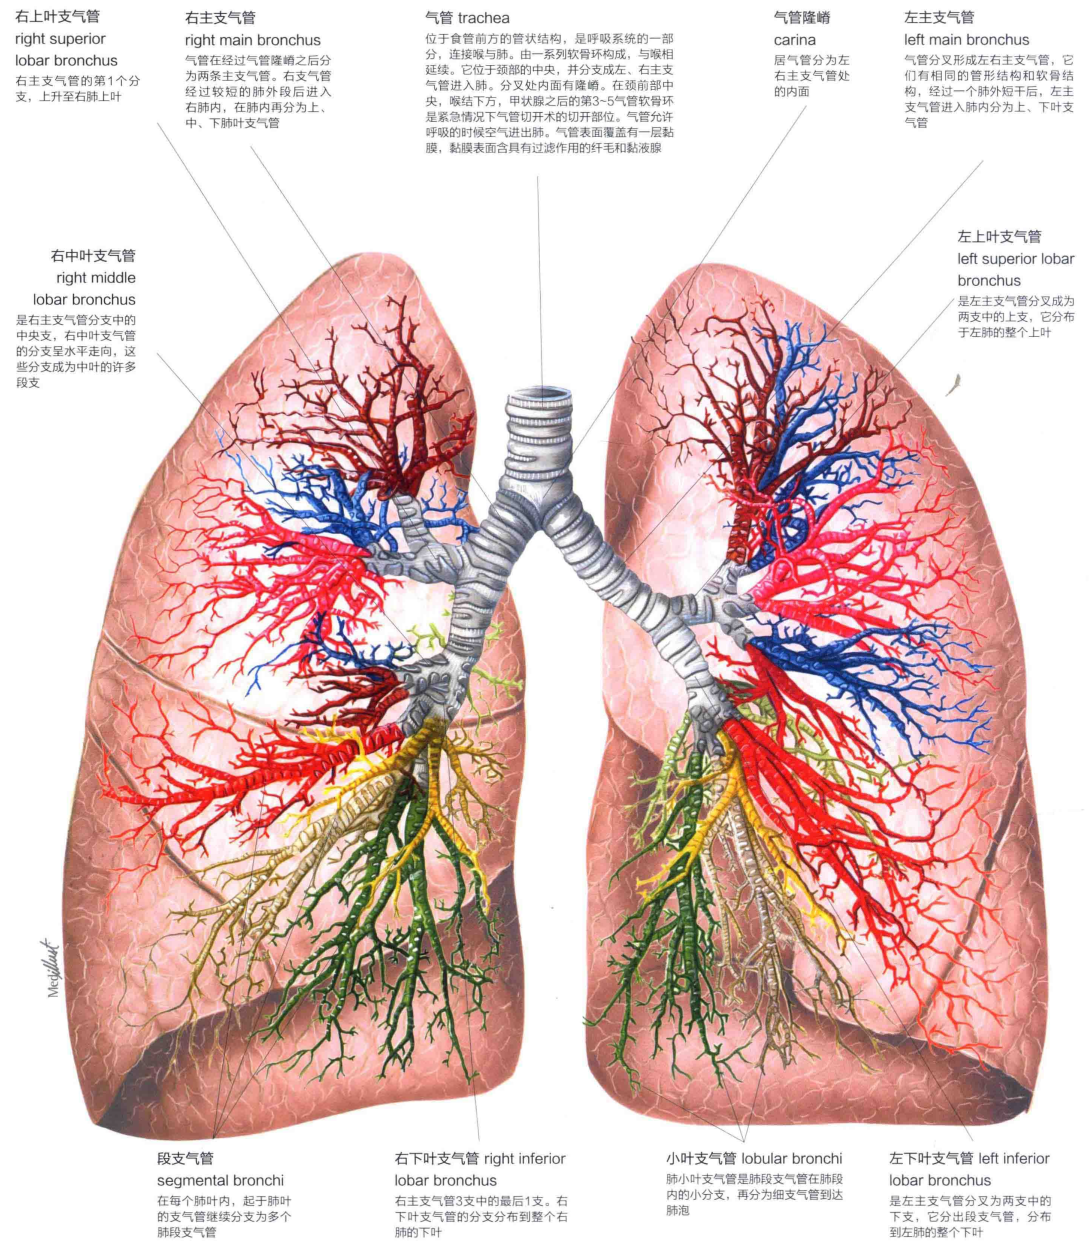
\includegraphics[width=0.9 \textwidth]{branches_of_the_bronchial_tree}
	\bicaption[肺部支气管气道树的分支结构]
		{肺部支气管气道树的分支结构\parencite{humananatomy2nd}}
		{The branch structure of pulmonary bronchial airway tree}
	\label{fig:branches_of_bronchial_tree}	
\end{figure}

如此繁复,从粗到细不断分化,面对如此稠密细小的支气管气道树,进行分割前需要经验丰富的临床专家进行非常细粒度的标注。手工标注耗费大量时间,
成本高昂且支气管越细小,标注越困难,易于出错。 标注任务艰巨繁重,急需开发新的算法或模型来帮助临床医生解决支气管气道树分割的问题。

\section{本研究的应用前景}

肺部支气管气道树的自动化分割是呼吸系统肺部疾病诊断治疗的一个重要问题和研究领域,在实际应用中具有非常重要的作用,提高医疗技术水平。当前,在
作者所在的医疗机器人行业,本研究项目有如下的应用前景:
\begin{itemize}
	\item {\heiti 导管手术机器人 }
	由于肺部支气管气道树三维模型具有精确的空间位置信息,CT扫描建立的坐标系赋予DICOM医疗图像每个像素都有相应的坐标位置信息,如图\ref{fig:coordinate}所示。
	\begin{figure}[!htp]
		\centering
		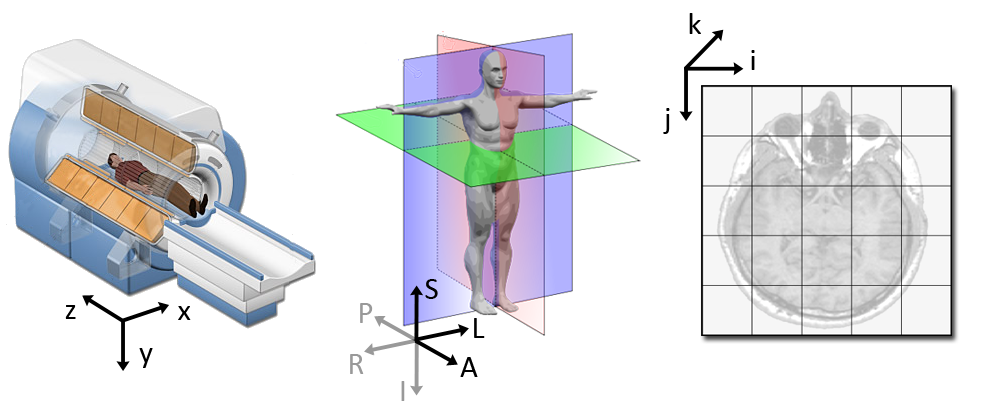
\includegraphics{Coordinate_sytems.png}
		\bicaption[CT扫描仪坐标系,人体坐标系和DICOM图像坐标系对应关系]
			{CT扫描仪坐标系,人体坐标系和DICOM图像坐标系对应关系\parencite{ctcoordinatesys2022, adaloglou2020dicomcoordinates}}
			{CT scanner, human body and DICOM imaging coordinates}
		\label{fig:coordinate}
	\end{figure}
	这样,分割出来的支气管气道树三维模型其每一个体素(Voxel)就具有精确的坐标位置信息,就可以计算出支气管管腔的中心线位置。
	
	导管机器人就是沿着管腔中心线的路径移动,导航至靶标位置。目前,美国Intuitive Surgical Company已经开发出肺部导管机器人ION,并投入了临床应用。
	\begin{figure}[!htp]
		\centering
		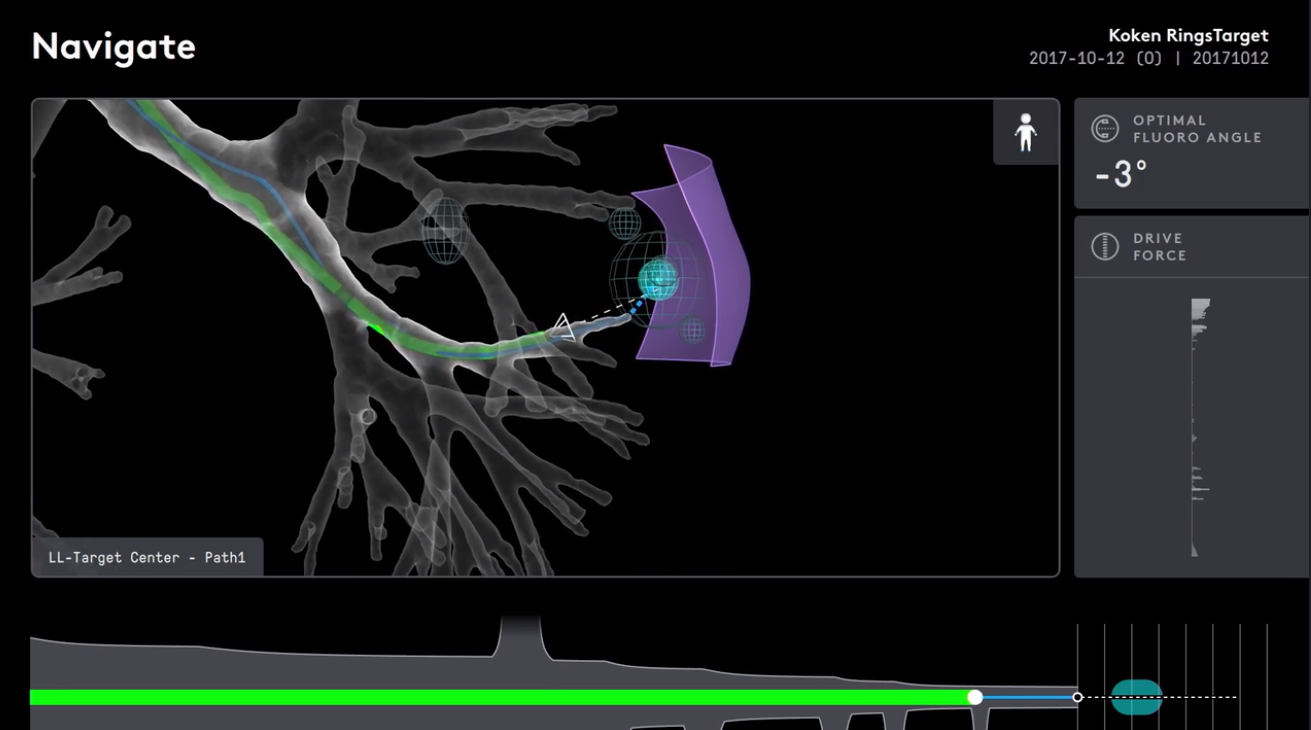
\includegraphics[width=0.45 \textwidth]{ION_robot_navigating}
		\hspace{2mm}
		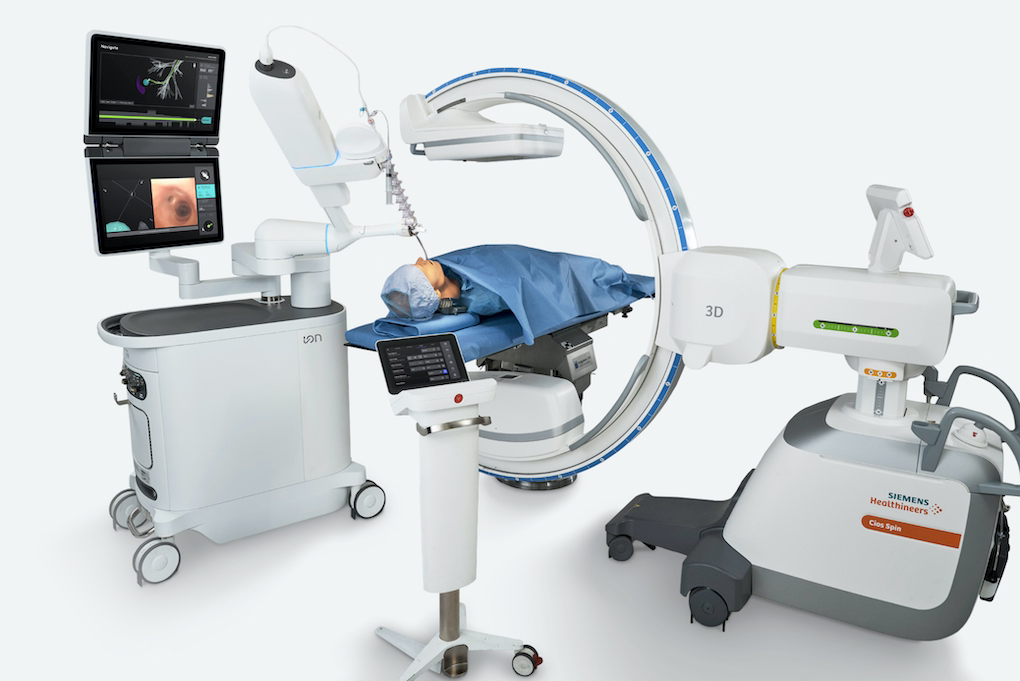
\includegraphics[width=0.45 \textwidth]{ION_bronchoscopy_robot.jpg}
		\bicaption[ION肺部导管机器人]
			{ION肺部导管机器人\parencite{ionrobot2021}}
			{ION bronchoscopy robot}
		\label{fig:ION_robot}
	\end{figure}
	
	作者所在的工作单位正在开发国产的肺部导管机器人,已经完成全国首例机器人辅助经支气管镜肺结节活检手术。
	
	当然导管手术机器人除了依赖支气管气道树三维模型导航,还需要辅助术中实时定位、支气管镜视觉导航的技术。
	
	
	\item {\heiti 智慧医疗辅助诊断}
	基于CT扫描图像的医疗图像分割需要高质量的标注数据,这很大程度上依赖经验丰富的临床医生/专家的专业知识。 为了减轻临床医生的标注压力和负担,同时亦为了减少误诊和漏诊
	的情况发生,医疗图像分割技术在医学辅助诊断上已经获得越来越多的应用。 具体到支气管气道树分割技术上,已经被用来辅助诊断一些慢性阻塞性肺部疾病COPD, 支气管扩张和肺气肿
	等一些肺部疾病。 随着AI图像分割技术的不断的进步,可以辅助临床医生更准确更高效地诊断疾病,逐渐达成智慧医疗,提高医疗技术水平和能力。
\end{itemize}



\section{研究现状和发展趋势}


图像分割技术已经发展很多年,从过去十年的发展来看,图像分割技术的发展经历了传统的图像分割方法和基于深度学习的分割方法2个阶段。传统的图像分割方法产生了一些比较经典的算法,
诸如基于阈值的最大类间方差Otsu方法\cite{otsu1979threshold},基于聚类的K-Means算法\cite{macqueen1965some}等。而随着近年来深度学习的发展,深度学习应用于图像分割
则是涌现了大量优秀的分割方法。Jonathan Long等人\cite{long2015fully}首次提出的全卷积网络(Fully Convolution Neural Network, FCN), 最经典的当属Olaf Ronneberger等人\cite{ronneberger2015u}提出的UNet结构,以及在UNet基础上改进提出的V-Net\cite{milletari2016v}结构模型、U-Net++\cite{zhou2019unet++}
结构模型,还有针对医疗影像这类三维体数据的分割模型3D UNet结构\cite{cciccek20163d},诸如这些基于深度学习的图像分割模型,其性能、精度、鲁棒性等指标都在不断进步,发展非常活跃。

下面分别介绍传统的图像分割方法、基于深度学习的图像分割方法和具体针对肺部支气管气道树的分割方法,了解他们的基本思想和发展趋势。

	\subsection{传统的图像分割方法}
	
	传统图像分割的方法是根据图像特征设计相应的算法对每个像素点进行分类,这些图像的特征包括颜色、纹理、亮度和形状等,其本质是根据特定标准确定一个合理的阈值,将每一个
	像素点与此阈值比较,以确定每一个像素点的分类。综合分析传统的图像分割方法,我们可以总结出如下的划分:
	\begin{enumerate}
		\item 阈值法
		
		阈值法是根据图像的灰度特征信息进行与阈值比较的计算。对欲分割的图像设定一个或多个(不同)的阈值,然后将图像上的每一个像素点与阈值进行比较,得到每个像素点所属的
		类别。这方面主要的工作有Sauvola法\cite{sauvola2000adaptive}、最大类间方差Otsu法\cite{otsu1979threshold}等。医疗图像(DICOM格式\cite{mustra2008overview})都是典型的灰度图\ref{fig:medical_image}。
		\begin{figure}[!htp]
			\centering
			\begin{subfigure}{\textwidth}
				\centering
				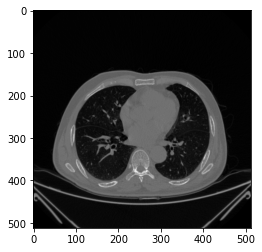
\includegraphics[scale=0.8]{DICOM image(axial view)}
				\caption{轴向面视图}
			\end{subfigure}
			
			\vspace{2mm}
			
			\begin{subfigure}{\textwidth}
				\centering
				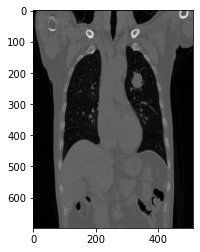
\includegraphics[scale=0.8]{DICOM image(coronal view)}
				\caption{冠状面视图}
			\end{subfigure}
			\bicaption[医疗图像(DICOM格式的灰度图)]
				{医疗图像(DICOM格式的灰度图)}
				{Medical image in DICOM format}
			\label{fig:medical_image}
		\end{figure}
		
		\item 区域法
		
		区域法是根据像素的灰度和纹理信息,以区域一致性规则进行分割。其包括:区域生长法、区域分裂、区域合并法。区域生长法通过指定一个种子点,向生长区域不断地添加满足
		约束条件的新的像素,直到填满或无法再添加。这些新添加进来的像素即属于一个类别,在不同的生长区域的像素从属于不同的类别。区域法初始形式简单,计算速度也快,它比较
		适合灰度均匀的图像分割。
		
		\item 聚类法
		
		聚类方法则根据像素间的特征相似程度进行迭代式的分类,将特征值相近的一组像素归为一个类别,然后计算这一组像素的中心位置。通过不断更新迭代直到完成所有像素的分类。
		这种方法的代表性工作便是K-Means算法\cite{macqueen1965some},聚类法使同类像素样本尽可能相近,而异类像素样本则拉大差异。聚类法的实现较为简单,但缺点就是
		对噪声很敏感,稍微不同的聚类中心和类别选择等因素都会导致分割结果差异,鲁棒性较差。
		
		\item 图论法
		
		图论法源于聚类的分割方法,它是将图像转换成带权重的无向图,将无向图划分为各种子图,使每个子图内部保持最大相似性,而子图之间则是差异尽可能大,每个子图代表
		一个类别。相关的图论分割方法就有归一化图分割、最小图分割、迭代式图分割等。
	\end{enumerate}
	
	\subsection{基于深度学习的图像分割方法}
	
	传统的图像分割方法围绕着图像的某一个具体特征进行精心挑选,设计与之匹配的算法,不具备广泛性和普遍性。 对于医疗的CT扫描图像,如前文图\ref{fig:medical_image}
	所述的都是对比度小的灰度图,传统的图像分割方法对于医疗图像不再适合。
	
	近年来随着深度学习技术在计算机视觉领域的应用,飞速发展并取得显著的进步。 基于深度卷积神经网络的语义分割方法对图像中的所有像素进行精确预测,预测像素属于哪一个类别
	的概率,赋予其标签,通过不断地迭代,从而分割出来图像。自美国加州大学UC Berkeley的Jonathan Long等人\cite{long2015fully}首次提出端到端、像素到像素的全卷积网络
	Fully Convolution Networks for Semantic Segmentation,取得的图像分割效果明显超过以往传统的图像分割法。以此为标志,打开了深度学习在图像分割领域应用的新通
	道。全卷积网络FCN由多个卷积层和池化层组合而成,学习图像中每个像素的语义信息,最后生成像素级的类别概率预测图。
	\begin{figure}[!htp]
		\centering
		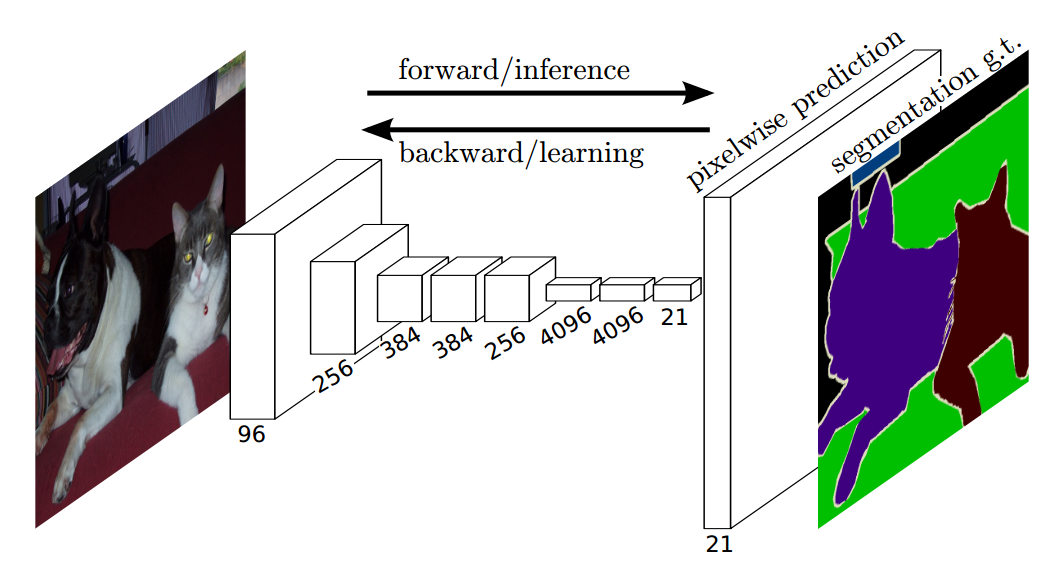
\includegraphics[width = 0.7 \textwidth]{FCN网络的结构}
		\bicaption[FCN网络的结构]
			{FCN网络的结构\cite{long2015fully}}
			{The structure of Fully Convolution Networks}
		\label{fig:FCN}
	\end{figure}
	
	但由于下采样路径上图像分辨率显著被降低,使得最后的预测结果比较粗糙。正如图\ref{fig:FCN}中分割结果只能看到2个物体的轮廓,无法看出是一只猫或是一只狗。在此基础上,
	Hyeonwoo Noh等人\cite{Noh2015LearningDN}添加进去了上采样路径,亦即反卷积Deconvolution,同步加入反池化Unpooling,将图像分辨率逐步恢复到原来的分辨率。
	\begin{figure}[!htp]
		\centering
		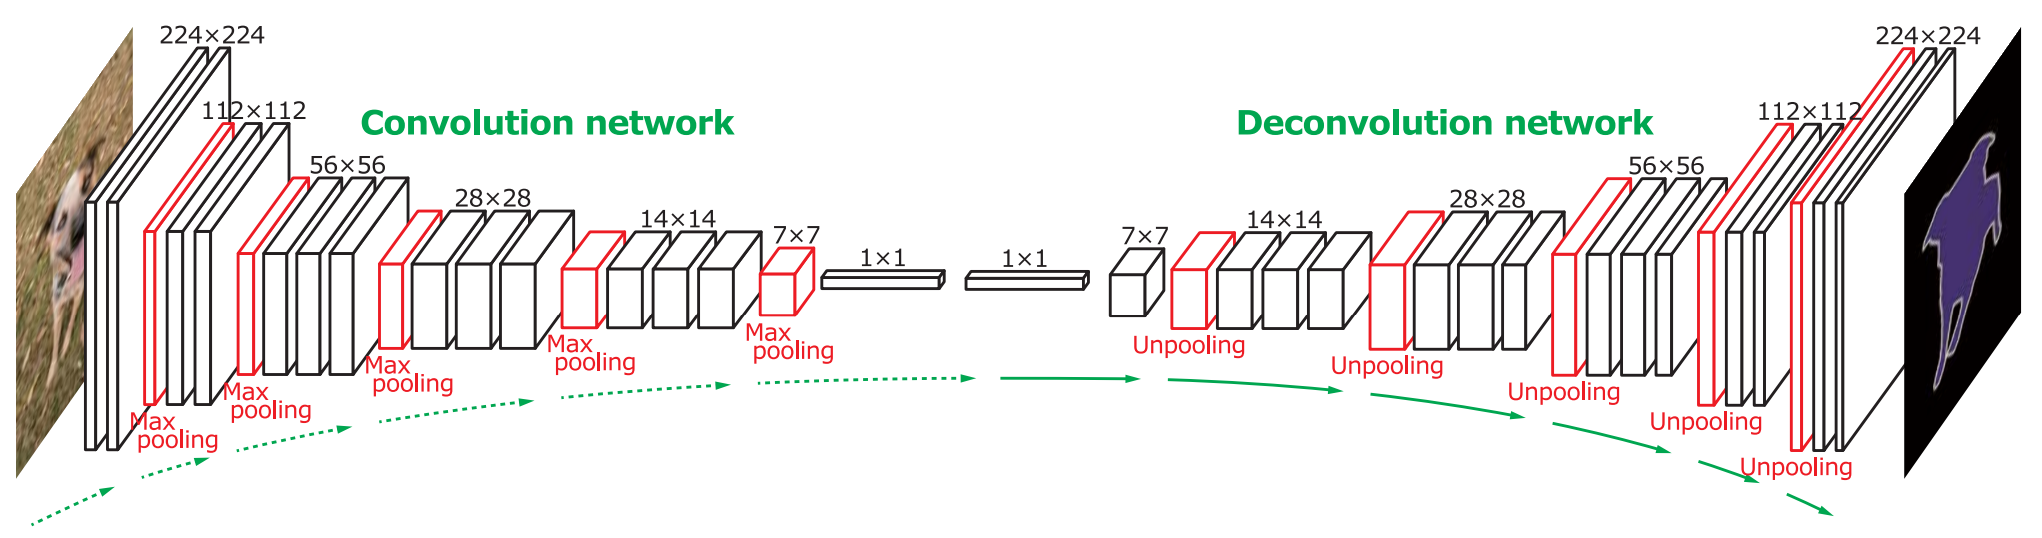
\includegraphics[width = 0.7 \textwidth]{Convolution_and_Deconvolution_network}
		\bicaption[卷积下采样路径 vs. 反卷积上采样路径]
			{卷积下采样路径 vs. 反卷积上采样路径\cite{Noh2015LearningDN}}
			{Convolutuion in down-samping path vs. Deconvolution in up-samping path}
		\label{fig:conv_deconv}
	\end{figure}
	\begin{figure}[!htp]
		\centering
		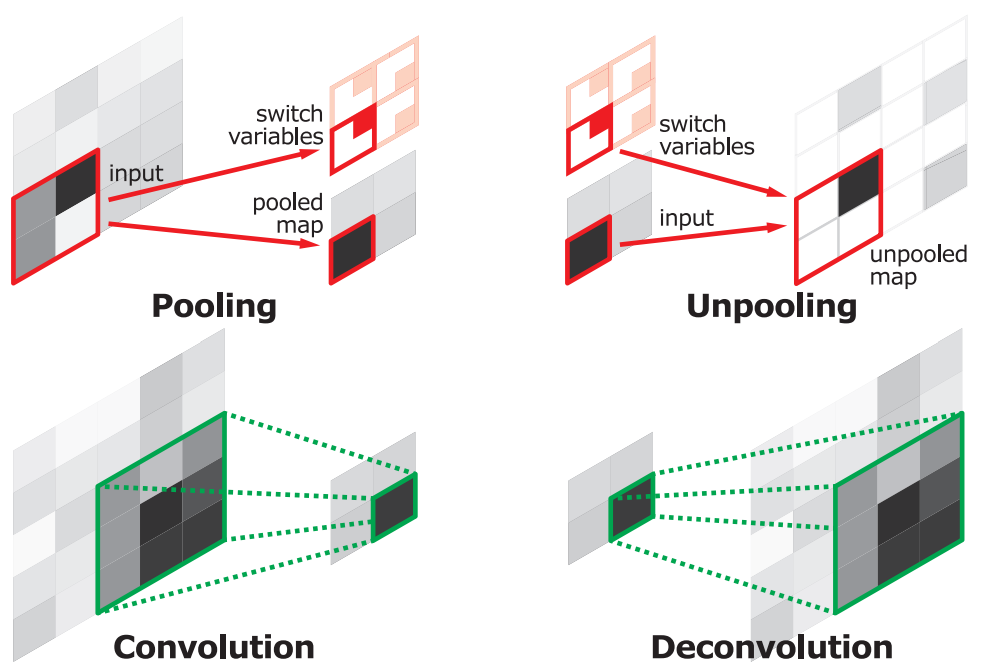
\includegraphics[width=0.6 \textwidth]{Deconvolution_and_unpooling_operations}
		\bicaption[卷积与反卷积,池化与反池化的操作]
			{卷积与翻卷积、池化与反池化的操作\cite{Noh2015LearningDN}}
			{The operations of convolution/deconvolution, and pooling/unpooling}
		\label{fig:conv_deconv_pooling_unpooling}
	\end{figure}
	
	图\ref{fig:conv_deconv}中的Convolution network与Deconvolution network也分别被成为编码器Encoder与解码器Decoder,这两条对称路径构成了Encoder-Deconder
	图像语义分割网络架构。
	
	后来,Olaf Ronneberger等人\cite{ronneberger2015u}则进一步改进,保留下采样路径用于提取深度特征信息,而在上采样路径则加入了跳跃连接,将下采样获取的深度特征信息
	跳跃过来与上采样拼接起来,实现特征图融合。这就是经典的U-Net网络结构。U-Net网络实现了更精细的图像语义分割结果。
	
	\begin{figure}[!htp]
		\centering
		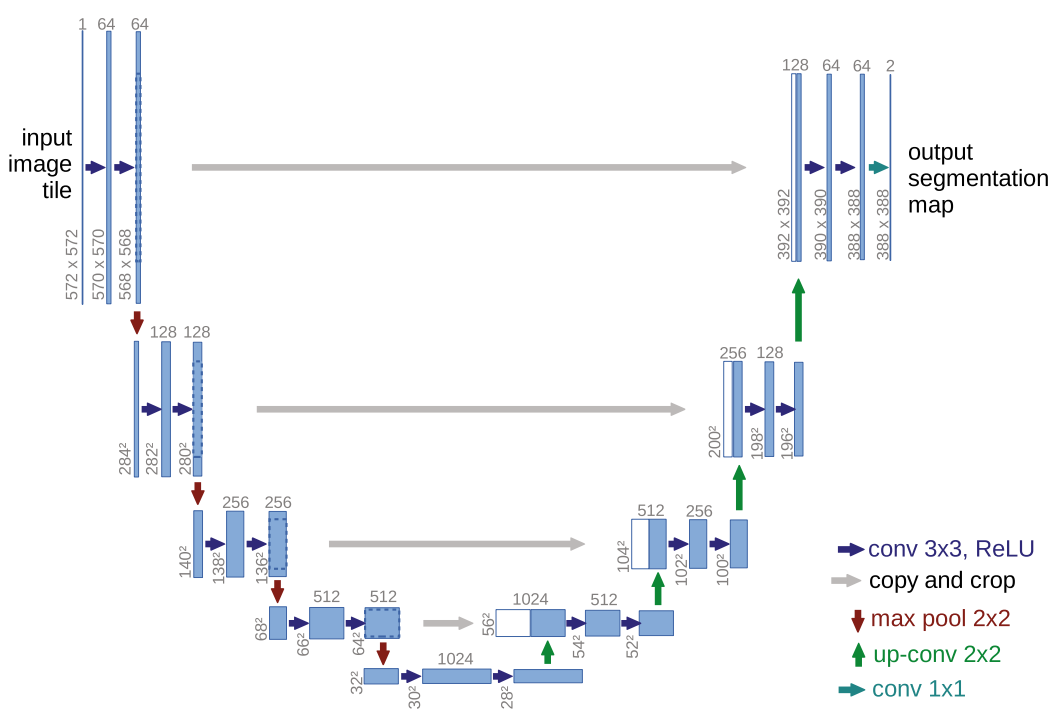
\includegraphics[width=0.7\textwidth]{UNet_architecture}
		\bicaption[经典的图像分割U-Net网络结构]
			{经典的图像分割U-Net网络结构\cite{ronneberger2015u}}
			{The classic U-Net architecture for image segmentation}
		\label{fig:UNet}
	\end{figure}
	
	U-Net网络目前已成为医疗图像分割任务的基础网络,有很多研究人员在U-Net基础上改进,应用在医疗图像的分割。比如肝脏、肺癌结节、乳腺肿块等不同的疾病。Li Xiaomeng等人
	\cite{Li2017HDenseUNetHD}提出一种基于U-Net混合式的稠密连接的新型网络结构H-DenseUNet用于肝癌的医疗CT图像的分割。它将UNet的保留低卷积层的细节特征,UNet网络
	越来越深的层次增加了训练的长耗时,而H-DenseUNet又可以解决这些深层网络的长耗时训练困难。
	
	医疗CT扫描图像基本上都是三维体数据,基于此又引申发展出3D CNN, Jose Dolz等人\cite{Dolze3DFCN}就提出了3D Fully convolutional networks, {\"O}zg{\"u}n {\c{C}}i{\c{c}}ek等人\cite{cciccek20163d}则提出3D UNet用于稠密的体数据分割。如此众多的分割网络,各个作者在UNet的基础上加上自己的创新,形成一个个独具特色的新型
	网络结构。那有没有一种广泛通用的网络来做图像分割呢? Mathias Perslev等人\cite{PerslevGeneralUNetFusion}就提出了这样的一个想法和实施方案
	One Network to segment them all一种通用	的轻量级的网络结构来精确分割3D图像。它是在UNet网络之后再加上一个Fusion model实现的。
	\begin{figure}[!htp]
		\centering
		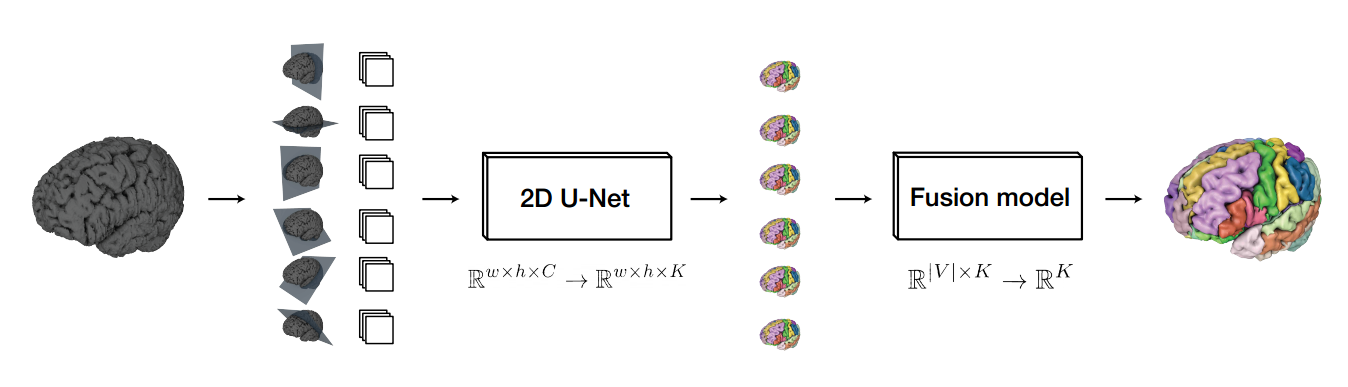
\includegraphics[width=0.8\textwidth]{Genral_UNet}
		\bicaption[一种通用的轻量化的UNet网络]
			{一种通用的轻量化的UNet网络\cite{PerslevGeneralUNetFusion}}
			{A general, lightweight UNet to segment them all}
		\label{fig:Genral_UNet}
	\end{figure}
	
	最近三年,新冠肺炎疫情肆虐全球,为了抗击疫情,许多研究人员的兴趣都被COVID-19吸引过去,争相研究感染了新冠病毒的肺部CT影像,以期帮助医疗专家、临床医生理解被感染
	后的肺部症状,预测是否感染了新冠肺炎。Zahid Ullah等人\cite{Ullah2023DenselyAM}提出一种稠密型注意力机制的网络来检测COVID-19的感染情况. 其网络结构(图
	\ref{fig:COVID19})在卷积层后插入通道注意力层和稠密区块层,使其聚焦于感兴趣的感染区域,从而高效地检测出感染情况。
	\begin{figure}[!htp]
		\centering
		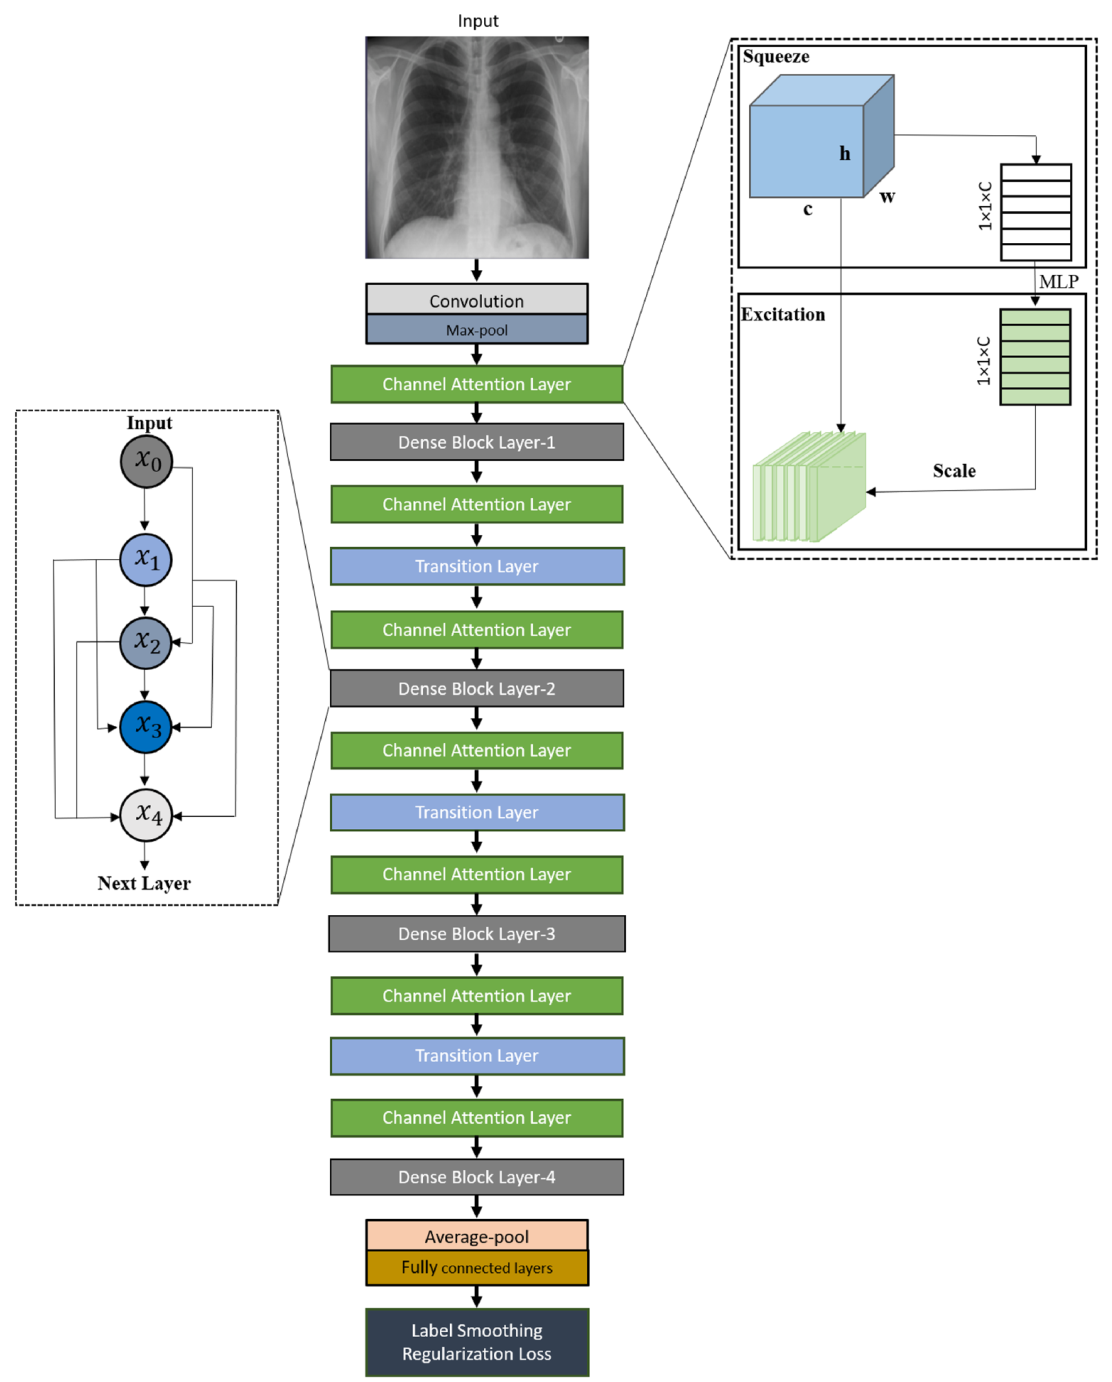
\includegraphics[width=0.5\textwidth]{Densely_attention_mechanism_based_network}
		\bicaption[稠密型注意力机制网络用来检测 COVID-19的感染情况]
			{稠密型注意力机制网络用来检测 COVID-19的感染情况\cite{Ullah2023DenselyAM}}
			{Densely attention mechanism network to detect the COVID-19 infection}
		\label{fig:COVID19}
	\end{figure}
	通过跟正常肺部影像和普通肺炎所造成阴影区域对比,比较明确地指出COVID-19感染区域(图\ref{fig:COVID19_detection}中COVID-19一栏所高亮显示的),展现给临床医生,辅助诊断是否感染新冠肺炎。
	\begin{figure}[!htp]
		\centering
		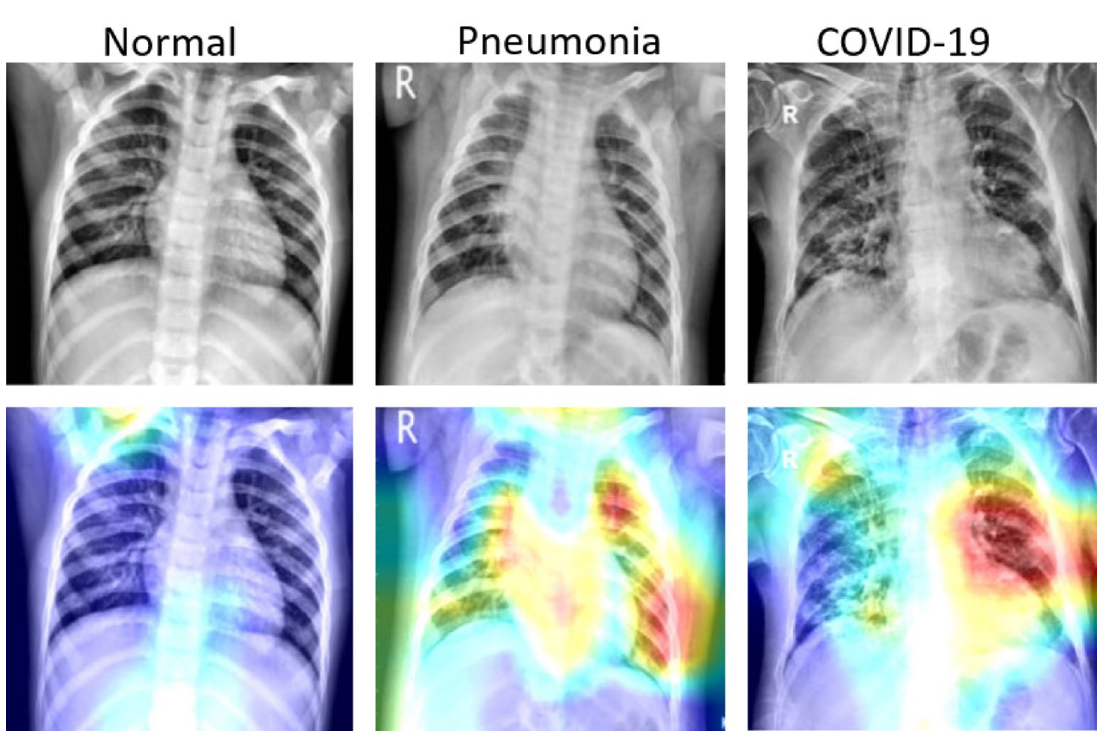
\includegraphics[width=0.8\textwidth]{Detect_COVID19_infection}
		\bicaption[对比正常肺部阴影、普通肺炎和COVID-19新冠肺炎的阴影,突出新冠肺炎感染区域]
			{对比正常肺部阴影、普通肺炎和COVID-19新冠肺炎的阴影,突出新冠肺炎感染区域\cite{Ullah2023DenselyAM}}
			{Highlight the COVID-19 infection area by comparing with normal and pneumonia}
		\label{fig:COVID19_detection}
	\end{figure}
	
	最新的进展是,随着NLP的Transformer模型\cite{Devlin2019BERTPO, NIPS2017Attention}取得成功后,NVIDIA的Ali Hatamizadeh和Vanderbilt Unversity的Yucheng Tang
	等人\cite{unetr}受此启发,率先将Transformer引入3D medical image segmentation中来,提出了UNETR网络结构(见图\ref{fig:UNETR}所示),实现了State-of-the-art (SOTA)医疗图像
	分割性能新记录。
	\begin{figure}[!htp]
		\centering
		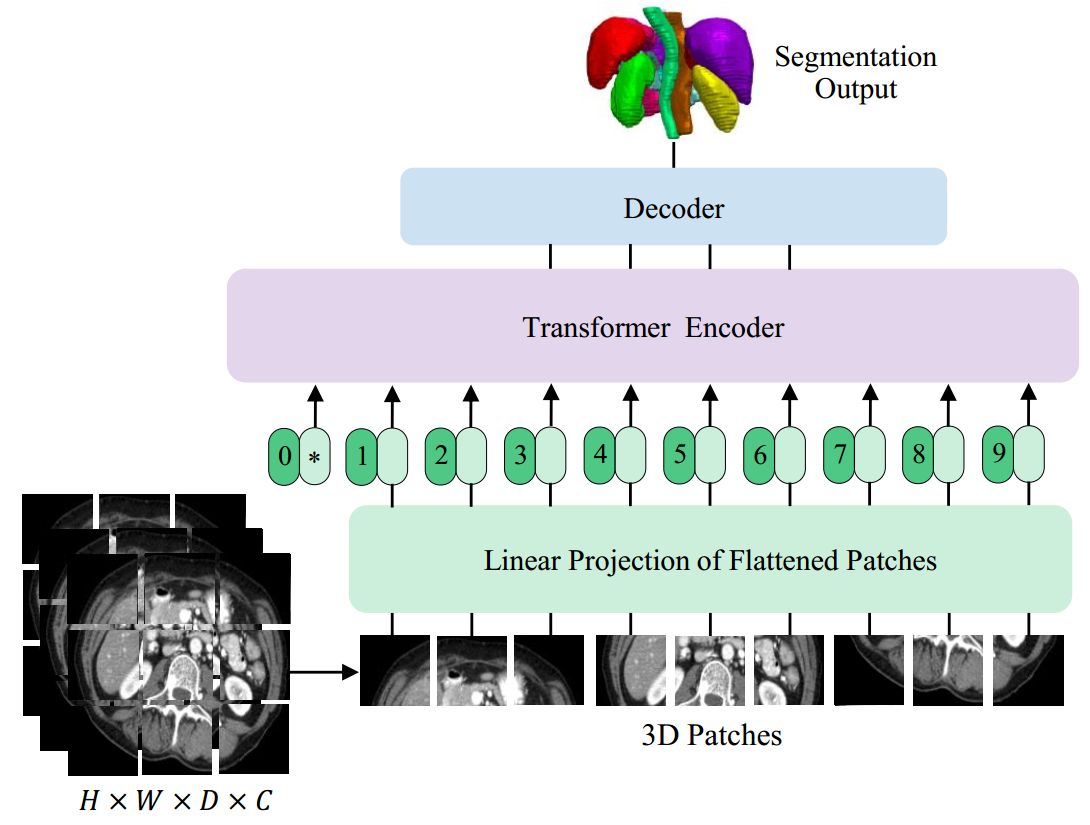
\includegraphics[width=0.6\textwidth]{Overview_of_UNETR}
		\bicaption[UNET网络基本结构]
			{UNETR网络基本结构\cite{unetr}}
			{The basic structure of UNETR network}
		\label{fig:UNETR}
	\end{figure}
	
	综上所述,基于深度学习的医疗图像分割技术发展非常活跃,研究进展迅速,进步巨大。
	
	
	
	\subsection{针对肺部支气管气道树的医疗图像分割方法}
	对于肺部CT图像的分割,卷积神经网络CNN早就应用在上面了。最知名的LUng Nodule Analysis 2016大挑战竞赛要求参赛选手分割出Lung CT图像的肺结节,判断肺结节是
	良性的还是恶性的,从而筛选出肺癌疑似患者,进行早期预防和针对性治疗。从LUNA16大挑战竞赛里诞生了两个具有重要影响力的公开数据集LUNA和LIDC-IDRI。 类似于LUNA
	大挑战竞赛,针对肺部支气管气道树的分割也有一个比较著名的EXtraction of Ariways from CT 2009 (EXACT'09)竞赛项目。Marleen de Bruijne等
	人\cite{Lo2012ExtractionOA}在2009年发起了EXACT'09这个竞赛项目,其研究目标就是提供一个公开通用的数据集,鼓励参赛选手开发出创新性算法,从胸部CT扫描图像中提取出
	支气管气道树,评比参赛选手门提交的算法。
	
	自EXACT'09大挑战竞赛的激励后涌现了大量的研究成果, Zhao Tianyi等人\cite{Zhao2019BronchusSA}开发出来一个两阶段2D + 3D的神经网络和一个基于线性规划的气道
	分割跟踪算法




























































\chapter{简介}

这是 \sjtuthesis 的示例文档,基本上覆盖了模板中所有格式的设置。建议大家在使用模
板之前,除了阅读《\sjtuthesis\ 使用文档》,这个示例文档也最好能看一看。

\section{二级标题}

\subsection{三级标题}

\subsubsection{四级标题}

Lorem ipsum dolor sit amet, consectetur adipiscing elit, sed do eiusmod tempor
incididunt ut labore et dolore magna aliqua. Ut enim ad minim veniam, quis
nostrud exercitation ullamco laboris nisi ut aliquip ex ea commodo consequat.
Duis aute irure dolor in reprehenderit in voluptate velit esse cillum dolore eu
fugiat nulla pariatur. Excepteur sint occaecat cupidatat non proident, sunt in
culpa qui officia deserunt mollit anim id est laborum.

\section{脚注}

Lorem ipsum dolor sit amet, consectetur adipiscing elit, sed do eiusmod tempor
incididunt ut labore et dolore magna aliqua. \footnote{Ut enim ad minim veniam,
quis nostrud exercitation ullamco laboris nisi ut aliquip ex ea commodo
consequat. Duis aute irure dolor in reprehenderit in voluptate velit esse cillum
dolore eu fugiat nulla pariatur.}

\section{字体}


上海交通大学是我国历史最悠久的高等学府之一,是教育部直属、教育部与上海市共建的全
国重点大学,是国家“七五”、“八五”重点建设和“211 工程”、“985 工程”的首批建
设高校。经过 115 年的不懈努力,上海交通大学已经成为一所“综合性、研究型、国际化”
的国内一流、国际知名大学,并正在向世界一流大学稳步迈进。 

{\songti 十九世纪末,甲午战败,民族危难。中国近代著名实业家、教育家盛宣怀和一批
  有识之士秉持“自强首在储才,储才必先兴学”的信念,于 1896 年在上海创办了交通大
  学的前身——南洋公学。建校伊始,学校即坚持“求实学,务实业”的宗旨,以培养“第
  一等人才”为教育目标,精勤进取,笃行不倦,在二十世纪二三十年代已成为国内著名的
  高等学府,被誉为“东方MIT”。抗战时期,广大师生历尽艰难,移转租界,内迁重庆,
  坚持办学,不少学生投笔从戎,浴血沙场。解放前夕,广大师生积极投身民主革命,学校
  被誉为“民主堡垒”。}

{\heiti 新中国成立初期,为配合国家经济建设的需要,学校调整出相当一部分优势专业、
  师资设备,支持国内兄弟院校的发展。五十年代中期,学校又响应国家建设大西北的号
  召,根据国务院决定,部分迁往西安,分为交通大学上海部分和西安部分。1959 年 3月
  两部分同时被列为全国重点大学,7 月经国务院批准分别独立建制,交通大学上海部分启
  用“上海交通大学”校名。历经西迁、两地办学、独立办学等变迁,为构建新中国的高等
  教育体系,促进社会主义建设做出了重要贡献。六七十年代,学校先后归属国防科工委和
  六机部领导,积极投身国防人才培养和国防科研,为“两弹一星”和国防现代化做出了
  巨大贡献。}

{\kaishu 改革开放以来,学校以“敢为天下先”的精神,大胆推进改革:率先组成教授代
  表团访问美国,率先实行校内管理体制改革,率先接受海外友人巨资捐赠等,有力地推动
  了学校的教学科研改革。1984 年,邓小平同志亲切接见了学校领导和师生代表,对学校
  的各项改革给予了充分肯定。在国家和上海市的大力支持下,学校以“上水平、创一流”
  为目标,以学科建设为龙头,先后恢复和兴建了理科、管理学科、生命学科、法学和人文
  学科等。1999 年,上海农学院并入;2005 年,与上海第二医科大学强强合并。至此,学
  校完成了综合性大学的学科布局。近年来,通过国家“985 工程”和“211 工程”的建
  设,学校高层次人才日渐汇聚,科研实力快速提升,实现了向研究型大学的转变。与此同
  时,学校通过与美国密西根大学等世界一流大学的合作办学,实施国际化战略取得重要突
  破。1985 年开始闵行校区建设,历经 20 多年,已基本建设成设施完善,环境优美的现
  代化大学校园,并已完成了办学重心向闵行校区的转移。学校现有徐汇、闵行、法华、七
  宝和重庆南路(卢湾)5 个校区,总占地面积 4840 亩。通过一系列的改革和建设,学校
  的各项办学指标大幅度上升,实现了跨越式发展,整体实力显著增强,为建设世界一流大
  学奠定了坚实的基础。}

{\ifcsname fangsong\endcsname\fangsong\else[无 \cs{fangsong} 字体。]\fi 交通大学
  始终把人才培养作为办学的根本任务。一百多年来,学校为国家和社会培养了 20余万各
  类优秀人才,包括一批杰出的政治家、科学家、社会活动家、实业家、工程技术专家和医
  学专家,如江泽民、陆定一、丁关根、汪道涵、钱学森、吴文俊、徐光宪、张光斗、黄炎
  培、邵力子、李叔同、蔡锷、邹韬奋、陈敏章、王振义、陈竺等。在中国科学院、中国工
  程院院士中,有 200 余位交大校友;在国家 23 位“两弹一星”功臣中,有 6 位交大校
  友;在 18 位国家最高科学技术奖获得者中,有 3 位来自交大。交大创造了中国近现代
  发展史上的诸多“第一”:中国最早的内燃机、最早的电机、最早的中文打字机等;新中国
  第一艘万吨轮、第一艘核潜艇、第一艘气垫船、第一艘水翼艇、自主设计的第一代战斗
  机、第一枚运载火箭、第一颗人造卫星、第一例心脏二尖瓣分离术、第一例成功移植同种
  原位肝手术、第一例成功抢救大面积烧伤病人手术等,都凝聚着交大师生和校友的心血智
  慧。改革开放以来,一批年轻的校友已在世界各地、各行各业崭露头角。}

{\ifcsname lishu\endcsname\lishu\else[无 \cs{lishu} 字体。]\fi 截至 2011 年 12
  月 31 日,学校共有 24 个学院 / 直属系(另有继续教育学院、技术学院和国际教育学
  院),19 个直属单位,12 家附属医院,全日制本科生 16802 人、研究生24495 人(其
  中博士研究生 5059 人);有专任教师 2979 名,其中教授 835 名;中国科学院院士 15
  名,中国工程院院士 20 名,中组部“千人计划”49 名,“长江学者”95 名,国家杰出
  青年基金获得者 80 名,国家重点基础研究发展计划(973 计划)首席科学家 24名,国
  家重大科学研究计划首席科学家 9名,国家基金委创新研究群体 6 个,教育部创新团队
  17 个。}

{\ifcsname youyuan\endcsname\youyuan\else[无 \cs{youyuan} 字体。]\fi 学校现有本
  科专业 68 个,涵盖经济学、法学、文学、理学、工学、农学、医学、管理学和艺术等九
  个学科门类;拥有国家级教学及人才培养基地 7 个,国家级校外实践教育基地 5个,国
  家级实验教学示范中心 5 个,上海市实验教学示范中心 4 个;有国家级教学团队 8个,
  上海市教学团队 15 个;有国家级教学名师 7 人,上海市教学名师 35 人;有国家级精
  品课程 46 门,上海市精品课程 117 门;有国家级双语示范课程 7 门;2001、2005 和
  2009 年,作为第一完成单位,共获得国家级教学成果 37 项、上海市教学成果 157
  项。}

% !TEX root = ../main.tex

\chapter{基准分割模型3D-UNet和分割效果分析}

\section{医疗图像语义分割基础}

图像的语义分割是一种像素级的分类技术,输入一张(RGB彩色或灰度)图片,分类器输出图片上每一个像素所属的类别标签。基于深度
学习的图像语义分割方法,其主要算法是卷积神经网络(Convolutional Neural Network, CNN)。卷积神经网络通常包含以下四层:
\begin{itemize}
    \item 卷积层 Convolution layer
    \item 归一化层 Normalization layer
    \item 激活函数层 Activation function
    \item 池化层 Pooling layer
\end{itemize}
CNN的基本网络结构如图\ref{fig:CNN_basic_structure}所示:
\begin{figure}[!htp]
    \centering
    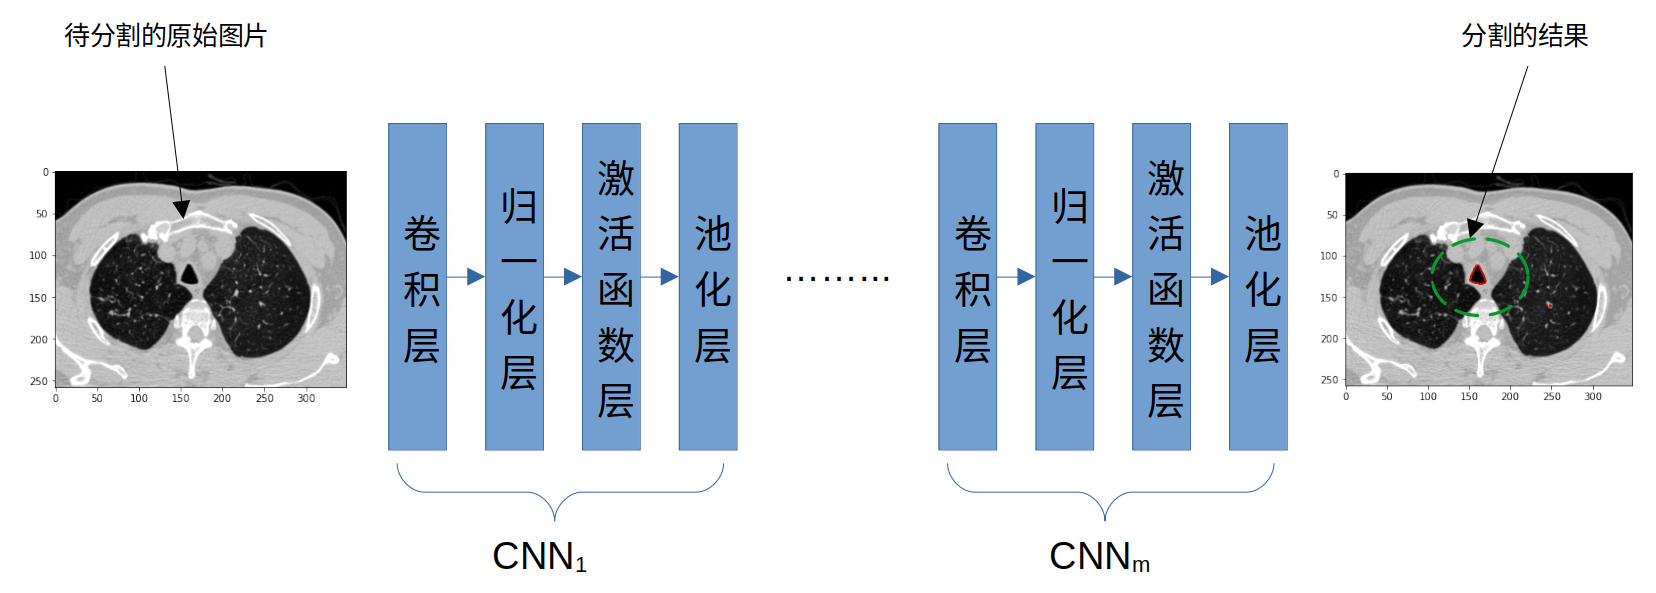
\includegraphics[width=\textwidth]{CNN_Structure}
    \bicaption[卷积神经网络基本构成]
        {卷积神经网络基本构成}
        {The basic structure of CNN}
    \label{fig:CNN_basic_structure}
\end{figure}

\noindent{}待分割的原始图片经过一层或连续多层的卷积网络后,图片的低层位置信息与高层语义信息等被提取出来,最后得到分割的结果。每次迭代
将预测的结果与真实的分割结果进行对比,选取一个合适的损失函数,计算损失值。然后通过梯度下降的反向传播,对卷积网络的参数---也就是
网络中每个神经元的权重Weight与偏置Bias---进行更新。循环进入下一次迭代,直到损失值不再降低趋于平缓,网络收敛,整个训练过程完成。

\subsection{卷积层}
卷积层的主要作用是提取特征,获得图像的局部信息。其工作原理是:在输入图像上滑动$H \times W = 3 \times 3$的窗口,每滑动
1个单位长度(此处滑动的长度称为步长Stride)就提取这个$3 \times 3$窗口内的像素信息,与同样尺寸的一个权重矩阵
(亦即卷积核尺寸convolution kernel size)做点积相乘并求和,得到当前位置的特征。

令$H3 \times W3$卷积核权重矩阵$W_{conv.kernel}$
\begin{equation}
    W_{conv.kernel} = \begin{bmatrix}
        w_1 & w_2 & w_3 \\
        w_4 & w_5 & w_6 \\
        w_7 & w_8 & w_9
    \end{bmatrix}
\end{equation}

CT扫描图像在$H3 \times W3$窗口内的Hounsfield unit\cite{HU2016CT}灰度\footnote{Hounsfield unit亨氏单位
是放射科医生在解释CT图像时使用的相对定量的无线电密度测量单位。CT重建时使用身体组织对辐射的吸收/衰减系数来生成灰度图像。
身体组织的物理密度与X射线束的吸收/衰减成正比。Hounsfield单位,也称为CT单位,是根据X射线束的线性衰减系数进行线性
变换计算而来的。}像素矩阵$X_{hu.gray}$
\begin{equation}
    X_{hu.gray} = \begin{bmatrix}
        x_1 & x_2 & x_3 \\
        x_4 & x_5 & x_6 \\
        x_7 & x_8 & x_9
    \end{bmatrix}
\end{equation}
则当前位置的特征$feat(X)$为
\begin{equation}\label{eq:conv}
\begin{split}
    {feat}(X) &= \sum{\left(W \cdot X\right)} + b \\
            &= \sum{\left(\begin{bmatrix}
                        w_1 & w_2 & w_3 \\
                        w_4 & w_5 & w_6 \\
                        w_7 & w_8 & w_9
                    \end{bmatrix} \cdot 
                    \begin{bmatrix}
                        x_1 & x_2 & x_3 \\
                        x_4 & x_5 & x_6 \\
                        x_7 & x_8 & x_9
                    \end{bmatrix}\right)} + b
\end{split}
\end{equation}
其中$b$为偏置参数Bias

式\ref{eq:conv}是在二维图像平面上的卷积操作,若在CT三维体数据上进行卷积运算,则卷积核尺寸扩展为$D3 \times H3 \times W3$
,相应地Hounsfield unit灰度像素矩阵也同步扩展到三维。三维卷积的操作如图\ref{fig:3D_Conv}所阐述:
\begin{figure}[!htp]
    \centering
    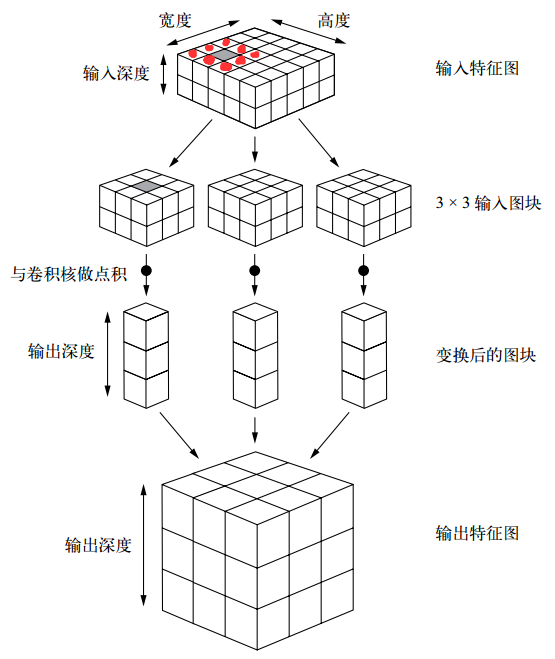
\includegraphics[width=0.5\textwidth]{Convolution_pricinple}
    \bicaption[三维卷积操作的原理]
        {三维卷积操作的原理}
        {The principle of 3D convolution}
    \label{fig:3D_Conv}
\end{figure}

\subsection{归一化层}
训练深度神经网络的计算强度非常大,训练时间漫长。减少训练时间的一种方法就是使网络中的神经元的活动归一化\cite{Ba2016LayerN}。
归一化是沿着某个指定的维度计算特征的均值与方差,对于推动深度网络收敛有着非常重要的作用。我们常用的归一化有:
\begin{enumerate}
    \item {批次归一化 Batch Normalization\cite{Ioffe2015BatchNA}}
    
    批次归一化是沿着Batch维度计算特征的均值和方差来进行归一化,批次的大小Batch size决定着预测的误差。通常取更大一些的Batch size
    有利于降低误差。过小的Batch size会导致性能下降。
    \item {层次归一化 Layer Normalization\cite{Ba2016LayerN}}
    
    层次归一化是沿着Channel维度计算特征的均值和方差来进行归一化。因为批次归一化依赖于Batch size, 尤其是不能低于mini batch size,
    而层次归一化是为了克服此问题的。
    \item {实例归一化 Instance Normalization\cite{Ulyanov2016InstanceNT}}
    
    实例归一化跟批次归一化执行相同的计算,但却是对单个样本而言。实例归一化可用于防止特定实例的均值和协方差偏移,简化学习过程。
    \item {群组归一化 Group Normalization\cite{Wu2018GroupN}}
    
    群组归一化是把Channel切分为组,在每个组内计算特征的均值和方差。群组归一化被Wu Yuxin等人\cite{Wu2018GroupN}提出来
    用于替换批次归一化,不同于层次归一化与实例归一化的方式,解决批次归一化对Batch size依赖的问题。
\end{enumerate}
我们可以用图\ref{fig:4norm}来讲解这4种归一化方式的差别。
\begin{figure}[!htp]
    \centering
    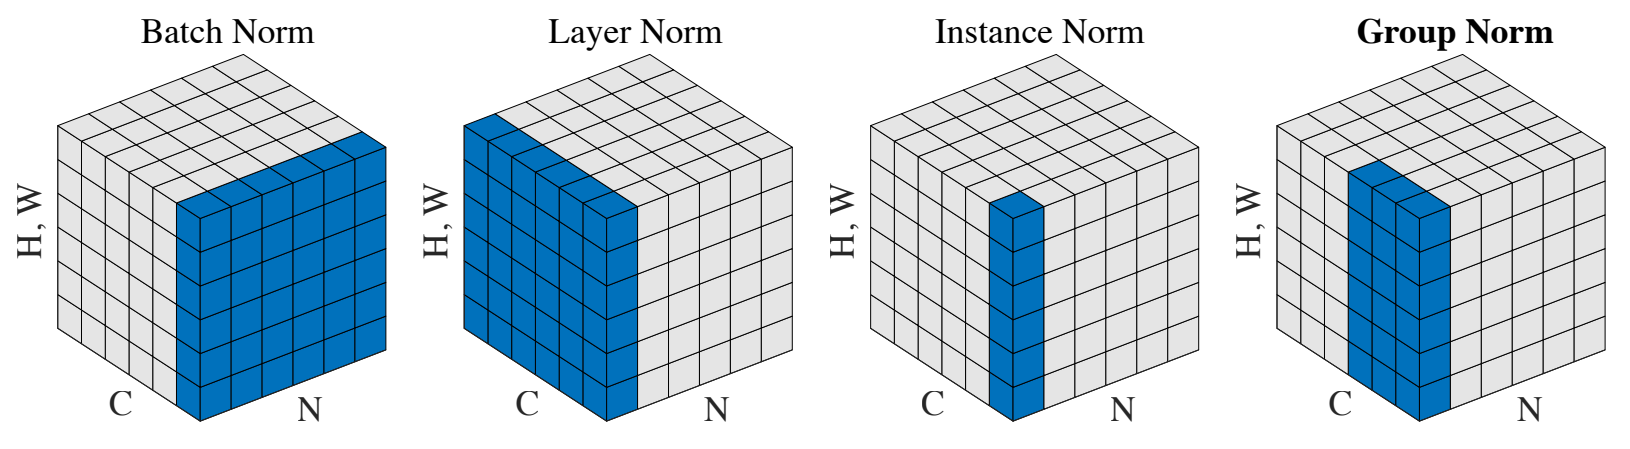
\includegraphics[width=\textwidth]{Four_Normalization_Methods}
    \bicaption[四种归一化方法的差别]
        {四种归一化方法\cite{Wu2018GroupN}}
        {Four Normalization Methods}
    \label{fig:4norm}
\end{figure}
深度网络的数据维度一般是$[Batch, Channel, Height, Width]$,简写为$[N, C, H, W]$($N$即为$Batch$)。
因为这是四个维度,我们无法画出一个四维空间的图形,所以压缩特征的$H, W$至一个维度。

\noindent{}批次归一化Batch Normalization沿Batch维度计算特征的均值和方差,归一化为$[N, H, W]$的维度,如图\ref{fig:4norm}
的Batch Norm子图的蓝色方格所示。

\noindent{}层次归一化Layer Normalization避开Batch维度,而是沿Channel维度计算特征的均值和方差,归一化为$[C, H, W]$的维度,
如图\ref{fig:4norm}的Layer Norm子图的蓝色方格所示。

\noindent{}实例归一化Instance Normalization选择单个样本计算特征的均值和方差,单个样本(也即一张图片)的维度只有$Height$
与$Weight$,所以归一化$[H, W]$的维度,如图\ref{fig:4norm}的Instance Norm子图的蓝色方格所示。

\noindent{}群组归一化Group Normalization则是介于层次归一化和实例归一化之间,其将$Channel$维度切分为很多组$Group$,
在每一个组内计算特征的均值和方差,归一化为$[C//G, H, W]$的维度,如图\ref{fig:4norm}的Group Norm子图的蓝色方格所示。

此外还有权重标准化(Weight Standardization\cite{Qiao2019WeightS})、 
批次-通道归一化(Batch-Channel Normalization\cite{Qiao2019RethinkingNA})、
深度归一化(DeepNorm\cite{Zare2017DeepNormADL})三种归一化方法,在此不做深入介绍。

\subsection{池化层}
池化的作用是缩小图像在高度和宽度方向上的空间运算,是一种降维的操作,可以用来改变当前层的输出维度,增大感受野。 池化有两种方式:
最大化池化Max Pooling和平均池化Average Pooling。最大化池化是从目标区域(图\ref{fig:pooling}的红色区域)中取出最大值,
平均池化则是计算目标区域(图\ref{fig:pooling}的深蓝色区域)的平均值。
\begin{figure}[!htp]
    \centering
    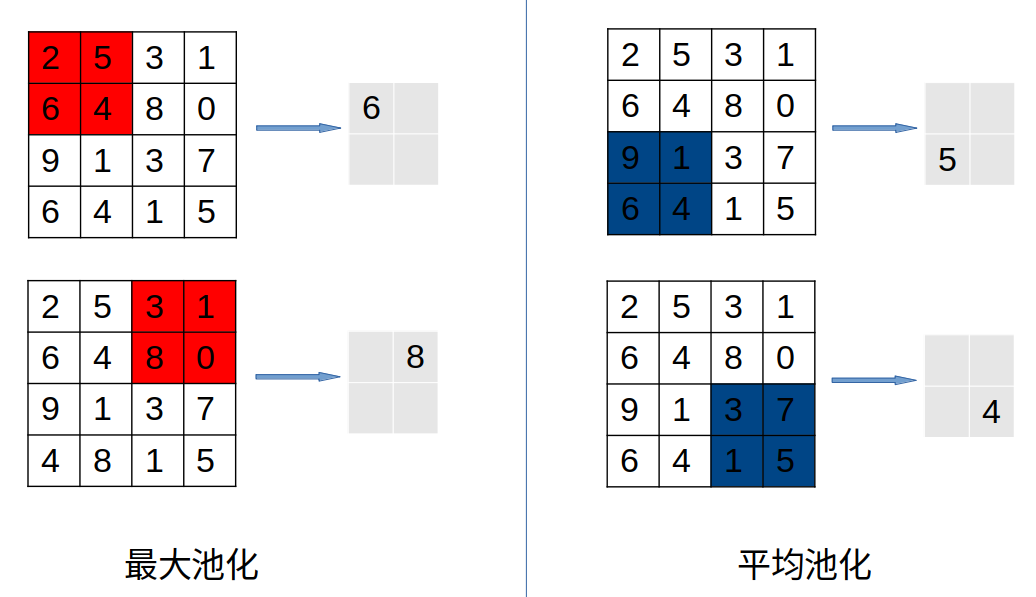
\includegraphics[width=0.7\textwidth]{Pooling}
    \bicaption[池化操作]
        {池化的基本操作}
        {The basic operations of pooling}
    \label{fig:pooling}
\end{figure}

池化层具有如下2个特征:
\begin{enumerate}
    \item {\heiti 没有要学习的参数}
    
    池化层与卷积层不一样,它没有要学习的参数。池化只是计算目标区域内的最大值或者平均值,所以不存在参数需要学习而改变。
    \item {\heiti 卷积的通道数保持不变}
    
    经过池化层,输入数据跟输出数据的通道数保持不变,是按照通道独立计算的。
    \begin{figure}[h]
        \centering
        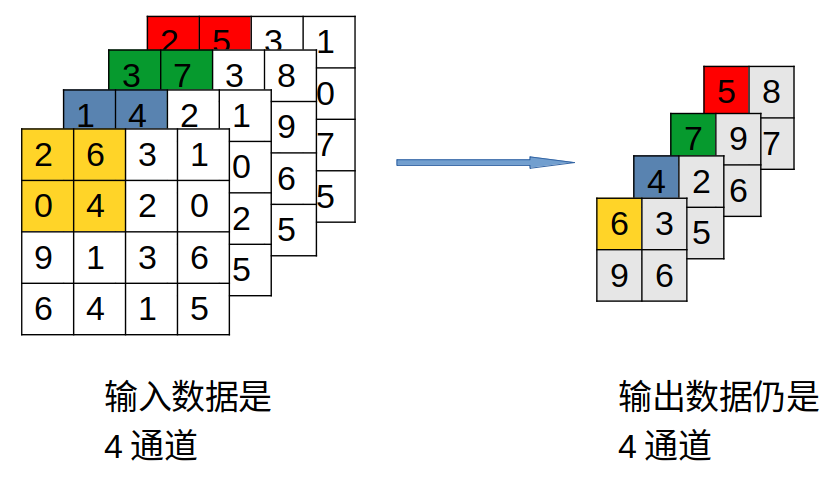
\includegraphics[scale=0.3]{Pooling_channels}
    \end{figure}
\end{enumerate}


\section{3D-UNet基准模型}
本文我们采用3D-UNet\cite{cciccek20163d}网络结构模型来分割支气管气道树,3D-UNet网络是将经典的UNet\cite{ronneberger2015u}
网络从平面图像分割扩展到三维体数据的。跟UNet网络的U型结构相似,我们将卷积层换成3D卷积,归一化层换成3D归一化,相应地池化层也更换为3D池化。
CT图像是一种体数据形式,它由一层一层的切片堆叠而成,每一层切片是一张二维的灰度图像。相比于平面图像中的像素,在CT图像中我们
定义体素Voxel为$D \times H \times W = 1 \times 1 \times 1$的立方体所含的像素,$D = 1$表明是一层切片。3D-UNet
网络的输入是$D \times H \times W$的体数据,我们称之为Cuboid,输出是每个体素的二分类分割概率图。我们在下采样路径上设计
4个卷积层块,每个卷积层块包含2层卷积。而在上采样路径上同样设计4个反卷积层块,每个反卷积层块包含2层反卷积。

\subsection{网络结构设计}

下采样路径上,每个卷积层块的结构如图\ref{fig:convblock}所示,将输入的体数据图像的通道数扩增一倍,从输入的$n$个特征通道
扩增到$2n$个特征通道。经过3D最大池化后,分辨率降低一半。
\begin{figure}[h]
    \centering
    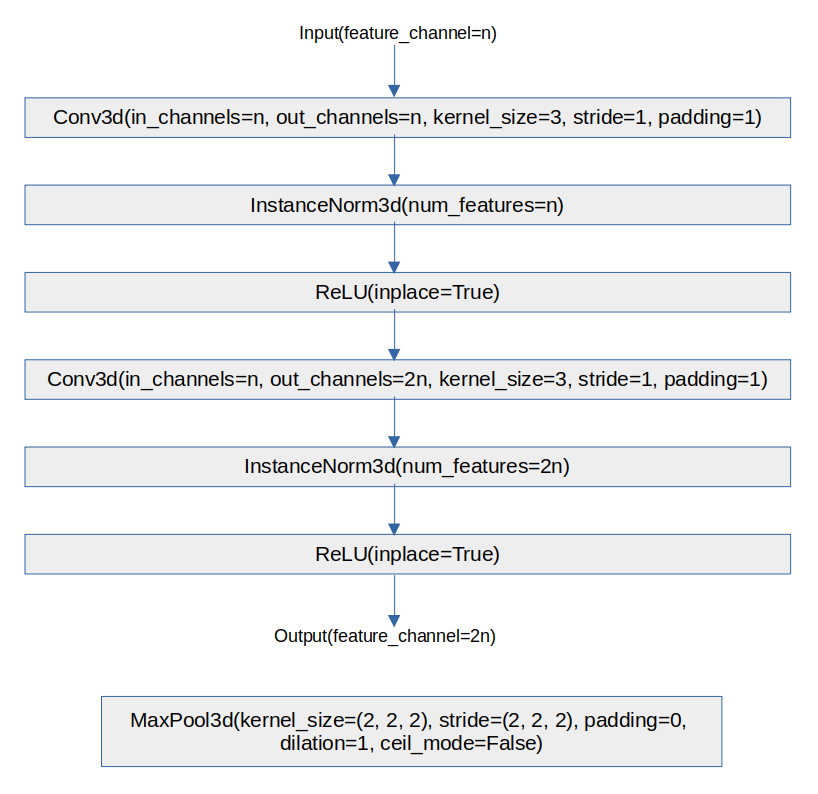
\includegraphics[width=0.8\textwidth]{Down_Conv_block}
    \bicaption[3D-UNet下采样路径上卷积层块和池化层的结构]
        {3D-UNet下采样路径上卷积层块和池化层的结构}
        {The convolution block and pooling layer in the down-sampling path of 3D-UNet}
    \label{fig:convblock}
\end{figure}

在上采样路径上,每个反卷积层块的结构如图\ref{fig:deconvblock}所示,将输入的体数据图像的通道数缩减一半。从输入的$n$个特征
通道缩减到$\frac{n}{2}$个特征通道。经过上采样池化后,分辨率升高一倍。将下采样路径降低的分辨率恢复起来,这样就实现端到端,
体素到体素的分割。
\begin{figure}[h]
    \centering
    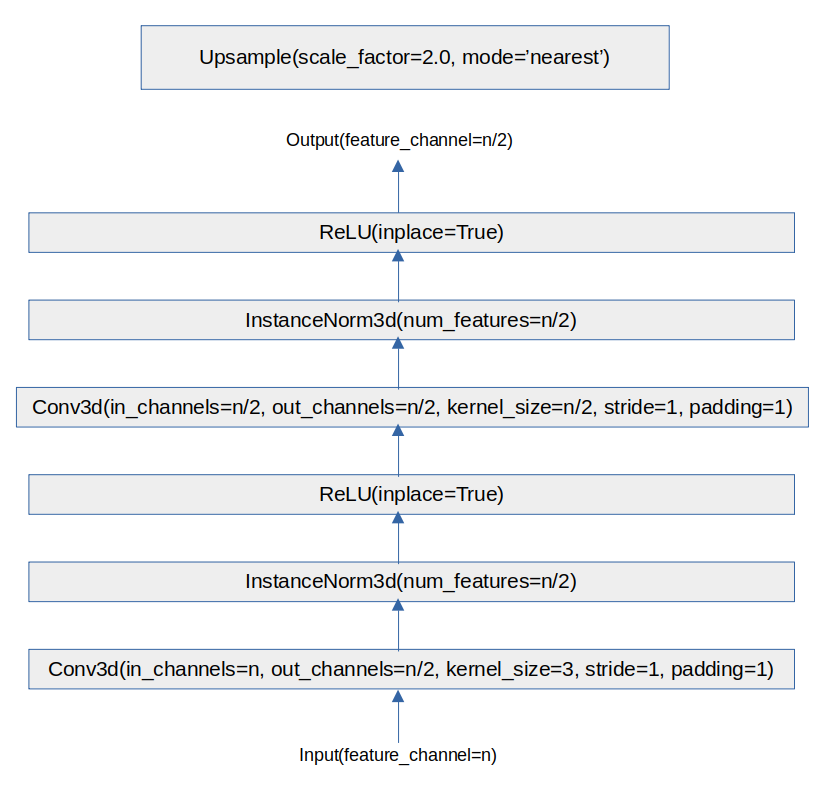
\includegraphics[width=0.8\textwidth]{Up_Conv_block}
    \bicaption[3D-UNet上采样路径上反卷积层块和池化层的结构]
        {3D-UNet上采样路径上翻卷积层块和池化层的结构}
        {The deconvolution block and pooling layer in the up-sampling path of 3D-UNet}
    \label{fig:deconvblock}
\end{figure}

我们的3D-UNet主干网络包括编码器Encoder和解码器Decoder两大部分,编码器主要用来实现图像的特征提取,扩大感受野,输出具有
类别信息的高层语义特征。解码器则逐步恢复分辨率,从而提取到低层的位置信息。更重要的是,在编码器和解码器对应的层次之间,引入
跳跃连接,将包含丰富细节信息的编码器特征拼接到解码器的高级分类特征信息中来,这样两种特征信息互相补充,最后输出每个像素的分类
概率图。我们的3D-UNet网络结构详情如图\ref{fig:3DUNetStructure}所示。由于图形宽度较大,我将其横向放置。将CT体数据(网络左侧)
\begin{figure}[ht]
    \centering
    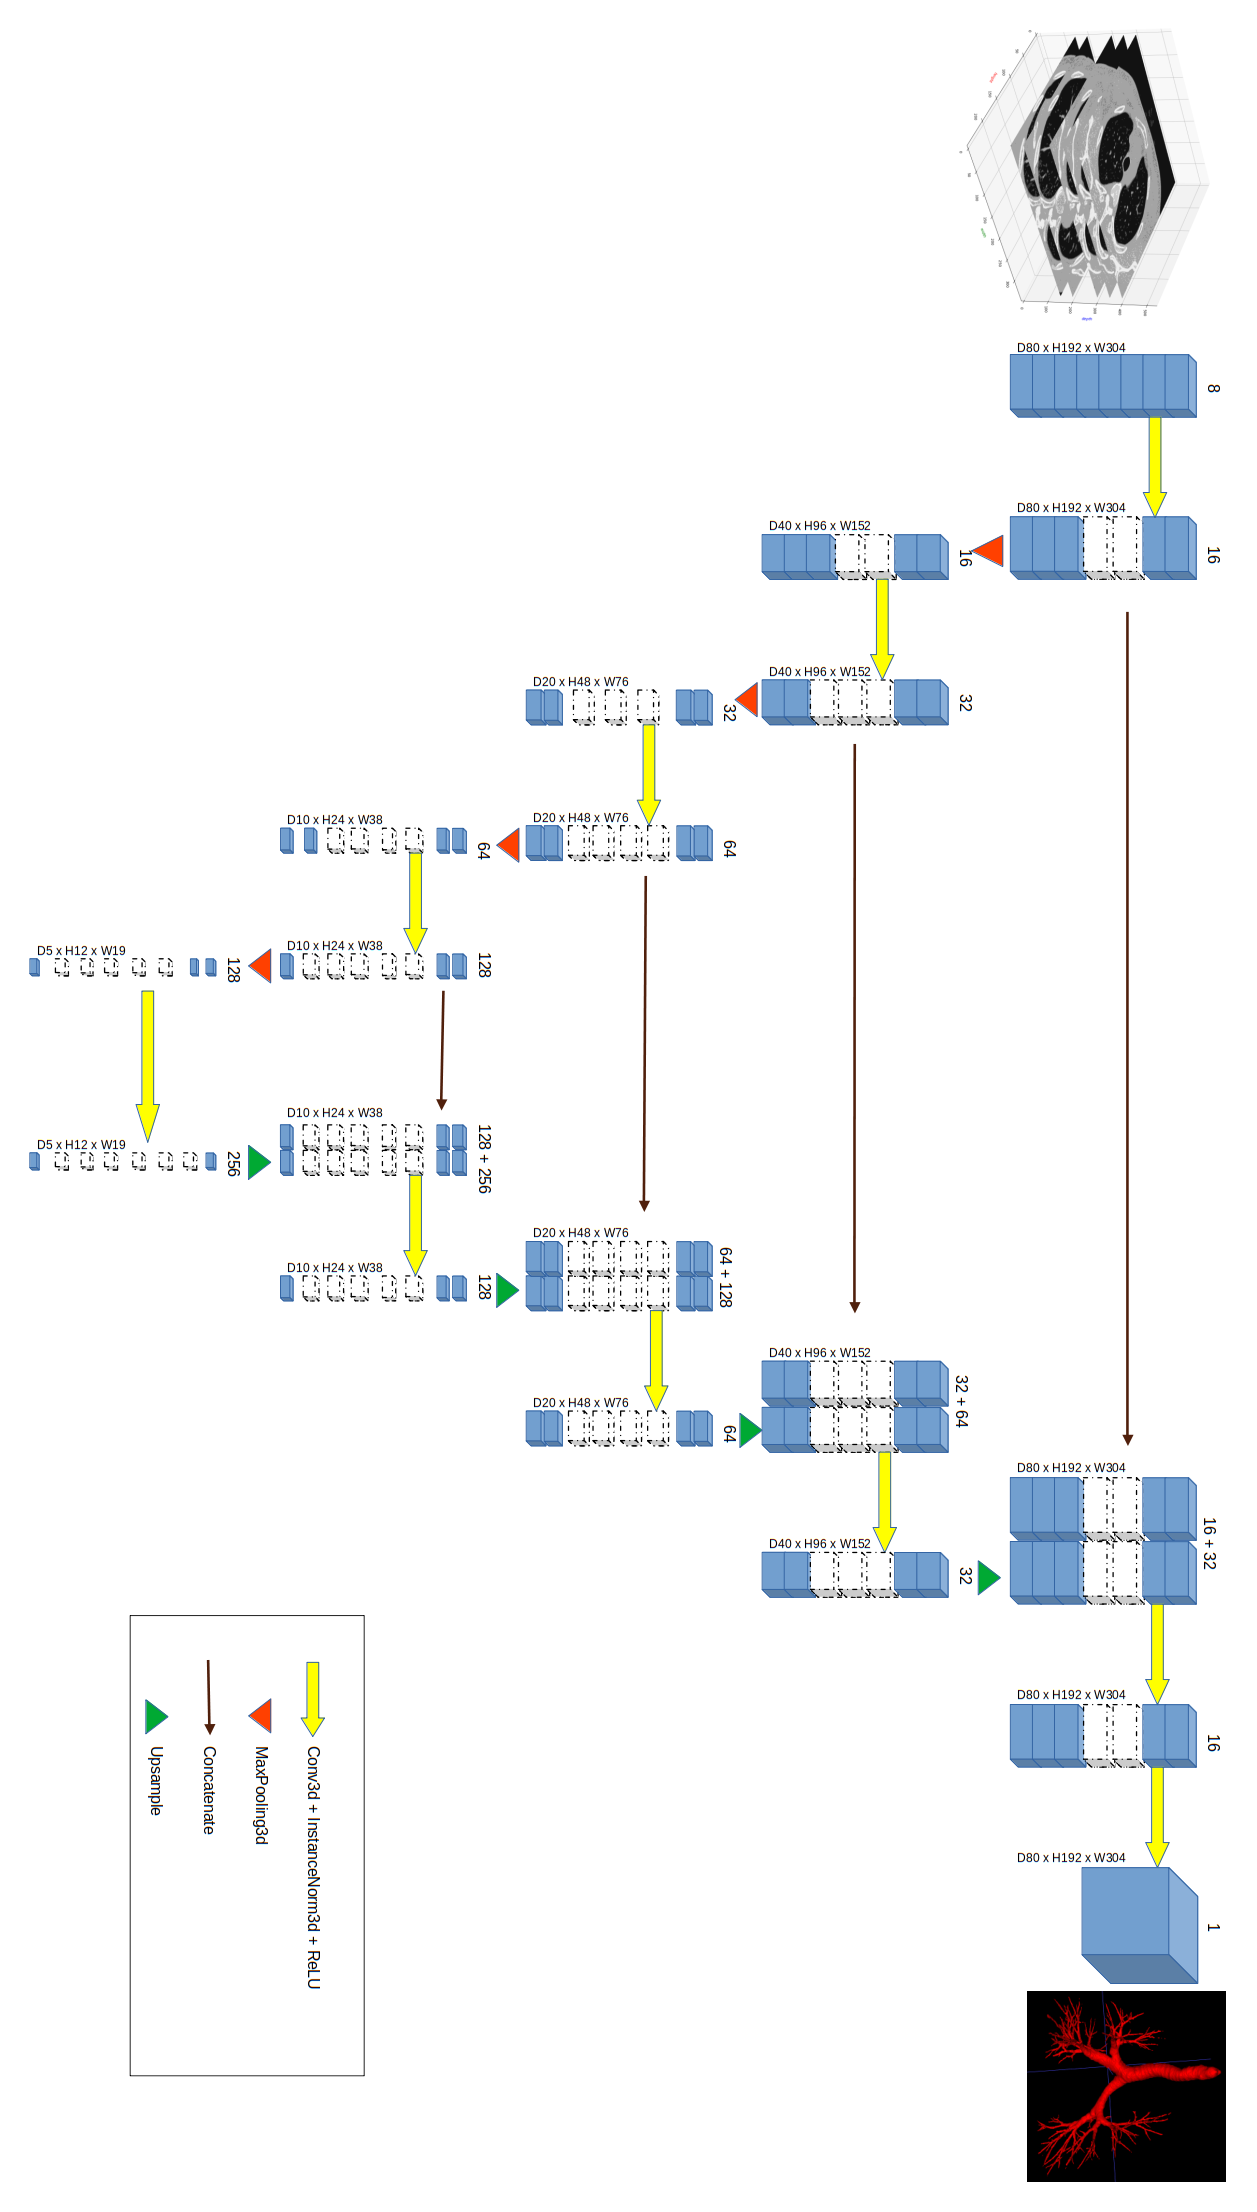
\includegraphics[height=0.72\textheight]{3DUNet_Structure_portrait}
    \bicaption[本文所设计与使用的3D-UNet网络结构]
        {本文所设计与使用的3D-UNet网络结构}
        {The 3D-UNet structure we designed in this paper}
    \label{fig:3DUNetStructure}
\end{figure}
送入网络之前,我们将其裁切为一个一个$D80 \times H192 \times W304$规格的长方体\footnote{我们将在后文讲述为什么裁切
成$D80 \times H192 \times W304$规格的。},网络学习长方体的图像特征,分割长方体内的支气管分支。训练完成后我们将属于同
一个原始CT图像的所有长方体拼接起来,最终分割出来完整的支气管气道树(网络右侧)。在长方体上面标出来的数字表示经过卷积操作后输出
的特征通道数,而在长方体侧面标注的诸如$D20 \times H48 \times W76$表示经过池化后,长方体的体积扩大或缩小,也就是长方体内
体素的分辨率增大或减小。需要指出的是,在U型结构的右侧,每一个层靠近跳跃连接的箭头处都有一个并排的长方体柱,那表示跳跃连接将
下采样路径上每一个卷积层块的特征输出拼接到上采样路径上每一个对应的反卷积层块的输入特征来。

上述的3D-UNet网络结构是本文所设计与使用,并编程实现的CT图像支气管气道树分割网络。我们将以此3D-UNet网络作为基准,通过实验
分析3D-UNet的分割结果和性能指标(包括但不限于假阳性率False Positive Rate、 真阳性率True Positive Rate、骰子相似度
系数Dice Similarity Coefficient、分支检出率Branch Detected、检测到的树长Tree Length Detected和精度等指标),提出
我们的改进方法。我们将在后面的章节展开讲述我们的改进方法,并通过实验来对比验证我们的改进方法是否有效,是否提高了分割效果和性能。

\subsection{损失函数、优化器与学习率调整}
\subsubsection{Dice损失函数}
我们为3D-UNet网络基准模型采用普遍的骰子损失函数Dice Loss, 其计算公式\ref{eq:dice_loss}
\begin{equation}\label{eq:dice_loss}
    L_{dice}\left(Cuboid_{pred}, Cuboid_{gt}\right) = 1 - \frac{2\sum{\left(Cuboid_{pred} \cdot Cuboid_{gt}\right)} + \epsilon}
    {\sum{Cuboid_{pred}} + \sum{Cuboid_{gt}} + \epsilon}
\end{equation}
其中${Cuboid}_{pred}$表示预测值三维矩阵,${Cuboid}_{gt}$表示真实值三维矩阵,此三维矩阵的大小为\ref{sec:ATM22dataset}
节中切割出来的长方体子块的大小$z \times y \times x = 80 \times 192 \times 304$. 而$\epsilon$是为防止除零而加入的平滑常数,
$Cuboid_{pred} \cdot Cuboid_{gt}$表示这2个三维矩阵的点积。

\subsubsection{Adam优化器与动态调整学习率}
支气管气道树分割是属于数据分布稀疏的场景,即有效的支气管体素在整个CT体素中的占比非常小,我们可以从ATM22数据集中随机挑选5个
病例,统计支气管体素在整个CT体素的占比来看稀疏程度。
\begin{table}[!htp]
    \bicaption[支气管体素占比]{支气管体素占比}{The percent of bronchus voxels over total voxels}
    \label{tbl:bronchus_voxels}
    \centering
    \begin{tabular}{crrr}
        \toprule
        病例名称 & 支气管体素 & 总体素 & 支气管体素占比 (\%)\\
        \midrule
        ATM\_009\_0000 &	 115,366 &	 209,453,056 &	 0.055 \\
        ATM\_027\_0000 &	 48,503  &	 161,218,560 &	 0.030 \\
        ATM\_016\_0000 &	 182,904 &	 187,170,816 &	 0.097 \\
        ATM\_033\_0000 &	 127,045 &	 171,704,320 &	 0.073 \\
        ATM\_023\_0000 &	 141,790 &	 209,453,056 &	 0.067 \\
        \bottomrule
    \end{tabular}
\end{table}
从表\ref{tbl:bronchus_voxels}可以看出,支气管体素占比都不到$0.1\%$,因此我们弃选随机梯度下降(Stochastic Gradient
Descend, SGD)优化器。为了更好地利用稀疏梯度信息,达到更好地收敛,我们选择Adam优化器。但是对Adam优化器,我们做了一些修改,
采用动态调整学习率。
让我们来看看Adam优化器\cite{Kingma2014AdamAM}计算梯度和更新参数的过程,来解释我们为什么采用动态调整学习率的方法。

\noindent{}网络模型的参数向量$\theta$在$t$时间步
\begin{equation}
\theta_{t} = \begin{bmatrix}
    \theta_{1} \\
    \theta_{2} \\
    \vdots      \\
    \theta_{n}
\end{bmatrix}_{t}
\end{equation}
计算在$t$时间步的梯度$grad_{t}$
\begin{equation}
    {grad}_{t} = \nabla_{t}J(\theta_{t})
\end{equation}
依据梯度的指数移动平均,计算在$t$时间步的一阶矩估计$m_{t}$
\begin{equation}
    m_{t} = \beta_{1} m_{t-1} + (1 - \beta_{1}) {grad}_{t}
\end{equation}
其中$\beta_{1}$为指数衰减率,控制权重分配、动量和当前梯度,默认取0.9。

\noindent{}依据梯度平方的指数移动平均,计算在$t$时间步的二阶矩估计$v_{t}$
\begin{equation}
    v_{t} = \beta_{2} v_{t-1} + (1 - \beta_{2}) {grad}_{t}^{2}
\end{equation}
其中$\beta_{2}$为指数衰减率,控制之前梯度的平方的影响,对梯度的平方进行加权平均,默认取0.999。

\noindent{}由于一阶矩估计$m_{t}$初始化为0,即$m_{0} = 0$,这会导致$m_{t}$偏向于0,特别是在训练早期阶段。为此我们需要对$m_{t}$进行
偏差纠正,降低偏差对训练早期的影响。
\begin{equation}
    \widehat{m_t} = \frac{m_t}{1 - \beta_{1}^{t}}
\end{equation}
其中$\beta_{1}^{t}$表示计算指数衰减率$\beta_{1}$的$t$次幂。

\noindent{}同样地,我们也需要对二阶矩阵估计$v_{t}$进行偏差纠正。
\begin{equation}
    \widehat{v_t} = \frac{v_t}{1 - \beta_{2}^{t}}
\end{equation}
$\beta_{2}^{t}$类似地表示对指数衰减率$\beta_{2}$的$t$次幂。

\noindent{}最后我们来更新在$t$时间步的参数$\theta_{t}$,学习率$lr$乘以梯度均值$\widehat{m_t}$与梯度方差的平方根
$\sqrt{\widehat{v_t}}$之比。为防止除零而引入平滑常数$\epsilon = 1 \times {10}^{-8}$
\begin{equation}\label{eq:adam_update_params}
    \begin{bmatrix}
        \theta_{0} \\
        \theta_{1} \\
        \vdots \\
        \theta_{n}
    \end{bmatrix}_{t} = 
    \begin{bmatrix}
        \theta_{0} \\
        \theta_{1} \\
        \vdots \\
        \theta_{n}
    \end{bmatrix}_{t-1} -
    {lr} * \frac{\widehat{m_t}}{\sqrt{\widehat{v_t}} + \epsilon}
\end{equation}
在式\ref{eq:adam_update_params}中,若分母$\sqrt{\widehat{v_t}}+\epsilon$过小,就会产生过大的参数$\theta_{t}$,
这会导致在接近最优值的“山峰”或“山谷”时会反复振荡,所以我们采取降低学习率的方法来稍微抵消一些。在训练的过程中,我们会逐渐地
动态地降低学习率。具体降低学习率的策略是:如果训练时的损失保持在一个平台超过10个epoch,我们就会降低学习率10倍, 
在训练后期我们会将这个周期拉长为20g个epoch。初始学习率设置为$3 \times {10}^{-3}$,动态降低学习率按照表
\ref{tbl:descend_lr}的规律来进行调整。
\begin{table}[!htp]
    \bicaption[动态降低学习率]{动态降低学习率}{Dynamically descent the learning rate}
    \label{tbl:descend_lr}
    \centering
    \begin{tabular}{cc}
        \toprule
        Epoch \# & Learning rate \\
        \midrule
        1 & $3 \times {10}^{-3}$ \\
        11 & $3 \times {10}^{-4}$ \\
        21 & $3 \times {10}^{-5}$ \\
        41 & $3 \times {10}^{-6}$ \\
        60 & $3 \times {10}^{-6}$ \\
        \bottomrule
    \end{tabular}
\end{table}


\subsection{模型实现和运行环境}
本文的模型是采用Python v3.10.9版本编写的,基于PyTorch v1.13.1框架实现3D-UNet模型的。本文的代码编写调试和模型训练均是
在上海交通大学高性能计算中心提供的AI超算平台上进行的。该AI超算平台由8台DGX-2组成,每台DGX-2配备16块NVIDIA Tesla V100显卡,
深度学习张量计算能力达到16PFLOPS。详细的配置与计算能力如表\ref{tbl:AT_platform}所示:
\begin{table}[!htp]
    \caption{人工智能超算平台资源}
    \label{tbl:AT_platform}
    \centering
    \begin{tabular}{c|l|c}
        \toprule
        队列 & 参数 & 节点数量 \\
        \midrule
        dgx2 & CPU: 2*Intel Xeon Scalable Cascade Lake 8168 (2.7GHz, 24 cores) & 8 (16卡/节点) \\
             & Memory: 1.5TB DDR4 ECC REG 2666 & \\
             & GPU: 16*NVIDIA Tesla V100 & \\
        \bottomrule
    \end{tabular}
\end{table}
本文的实验被分配最多8块显卡,由于有多个对比实验同时运行,因此不是8块显卡被一个实验独占使用。一般地我为轻计算量的实验分配2块
显卡,为重计算量的实验分配4块显卡。这样在同一个时间段就可以同时执行多个计算任务,使对比实验可以并行进行。

由于本文的实验是在超级计算机上执行,完全不同于传统的普通台式机、工作站等环境,因此有必要讲解清楚本文的实验运行环境。AI超算平台
使用Slurm作业调度系统(如图\ref{fig:slurm_job_system})来执行超算用户提交的计算任务,用户需要编写专有的Slurm作业脚本来提交作业请求。
\begin{figure}[!htp]
    \centering
    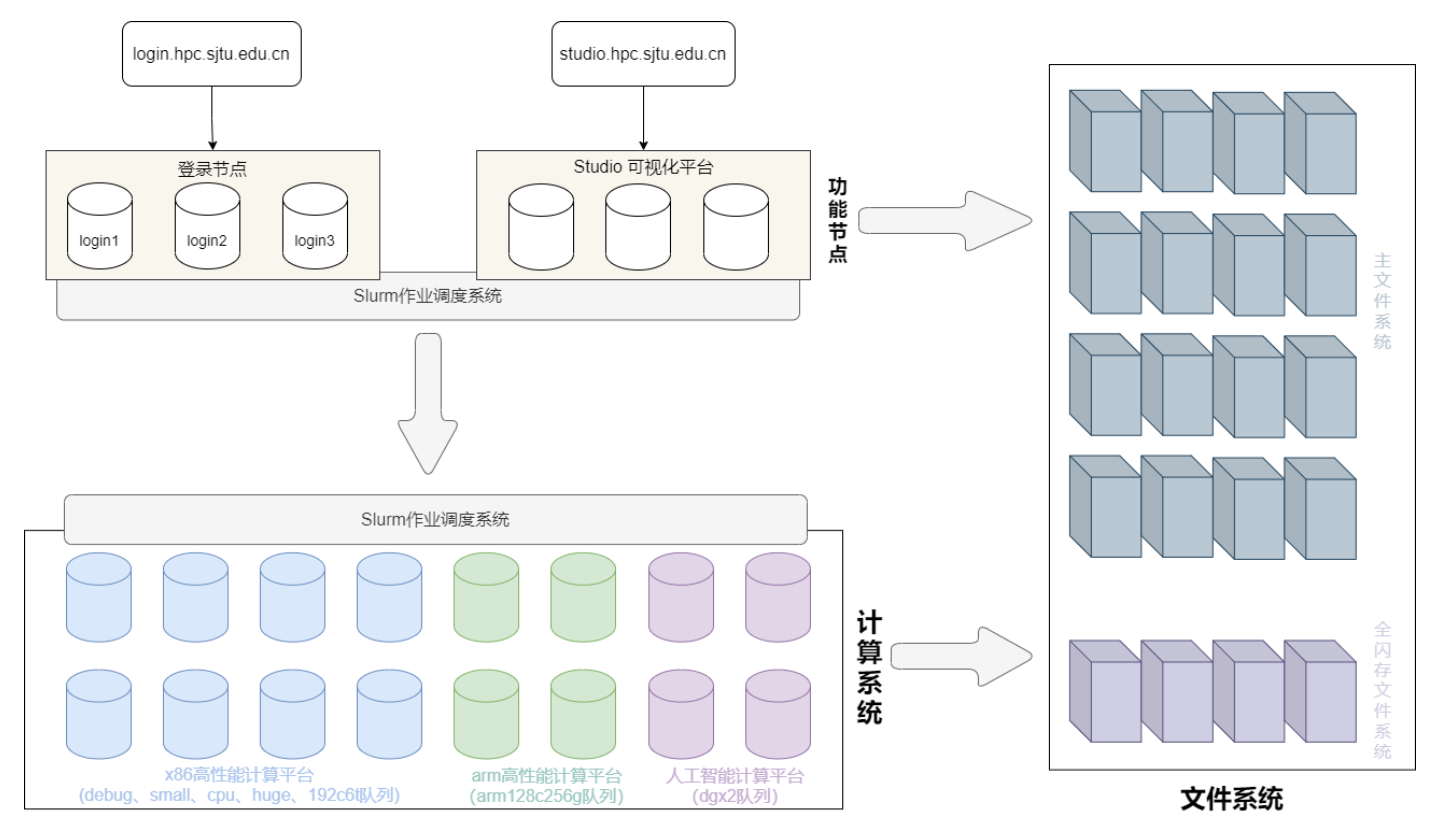
\includegraphics[width=0.8\textwidth]{Supercomputer_Slurm_Job_system}
    \bicaption[AI超算平台Slurm作业调度系统]
        {AI超算平台Slurm作业调度系统\parencite{HpcSlurm2022}}
        {The Slurm job scheduling system on AI supercomputer platform}
    \label{fig:slurm_job_system}
\end{figure}
Slurm脚本里指定当前作业需要用到的CPU核数,需要用到多少张GPU显卡,多少个进程,占用多少个计算节点。这是大规模并行计算需要指定
的计算资源。除此之外,还要配置Python-PyTorch环境,用户准备好可执行程序启动方式,设置好参数选项。最后通过 
\$sbatch Airway3DSegment\_Baseline.slurm命令提交作业,Slurm作业调度系统分配好计算资源后才开始执行计算任务。

\section{数据集ATM22}\label{sec:ATM22dataset}\label{sec:ATM22}
本文使用的数据集是公开的ATM22数据集\cite{Zhang2022CFDA, Zhang2021Airway, Yu2022Bronchi, Qin2019AirwayNet},
是由上海交通大学医疗机器人研究院联合上海胸科医院从多家医疗机构,多台不同品牌型号的CT扫描仪收集500例就诊者的胸腔扫描图像,然后
由三名具有五年以上专业经验的放射科医生对气道树结构进行精细的标注。ATM22数据集融合了EXACT'09数据集和LIDC-IDRI部分病例
的数据。我们随机选取了66例CT扫描图像作为训练集, 9例作为验证集,19例作为测试集。训练集、验证集和测试集的比例基本按照70:10:20
的比例来。由于ATM22数据集是采自不同医疗机构、不同品牌型号的CT扫描仪,因此我们对数据进行了预处理,将这些CT图像的体素强度统一截断
在$[-1000, 400]$亨式单位Hounsfield unit的窗口范围内,并归一化到$[0, 1]$范围。

ATM22数据集里的CT图像切片的尺寸基本都是H512 $\times$ W512个像素,存在很大面积的黑色背景,为了避免学习到肺部之外的无关
区域,我们对其进行裁切,只保留肺的最小包围框作为有效的区域,“喂给”深度网络进行学习。裁切前后的肺部区域效果对比如图
\ref{fig:cropimage}所示,
\begin{figure}[htbp]
    \centering
    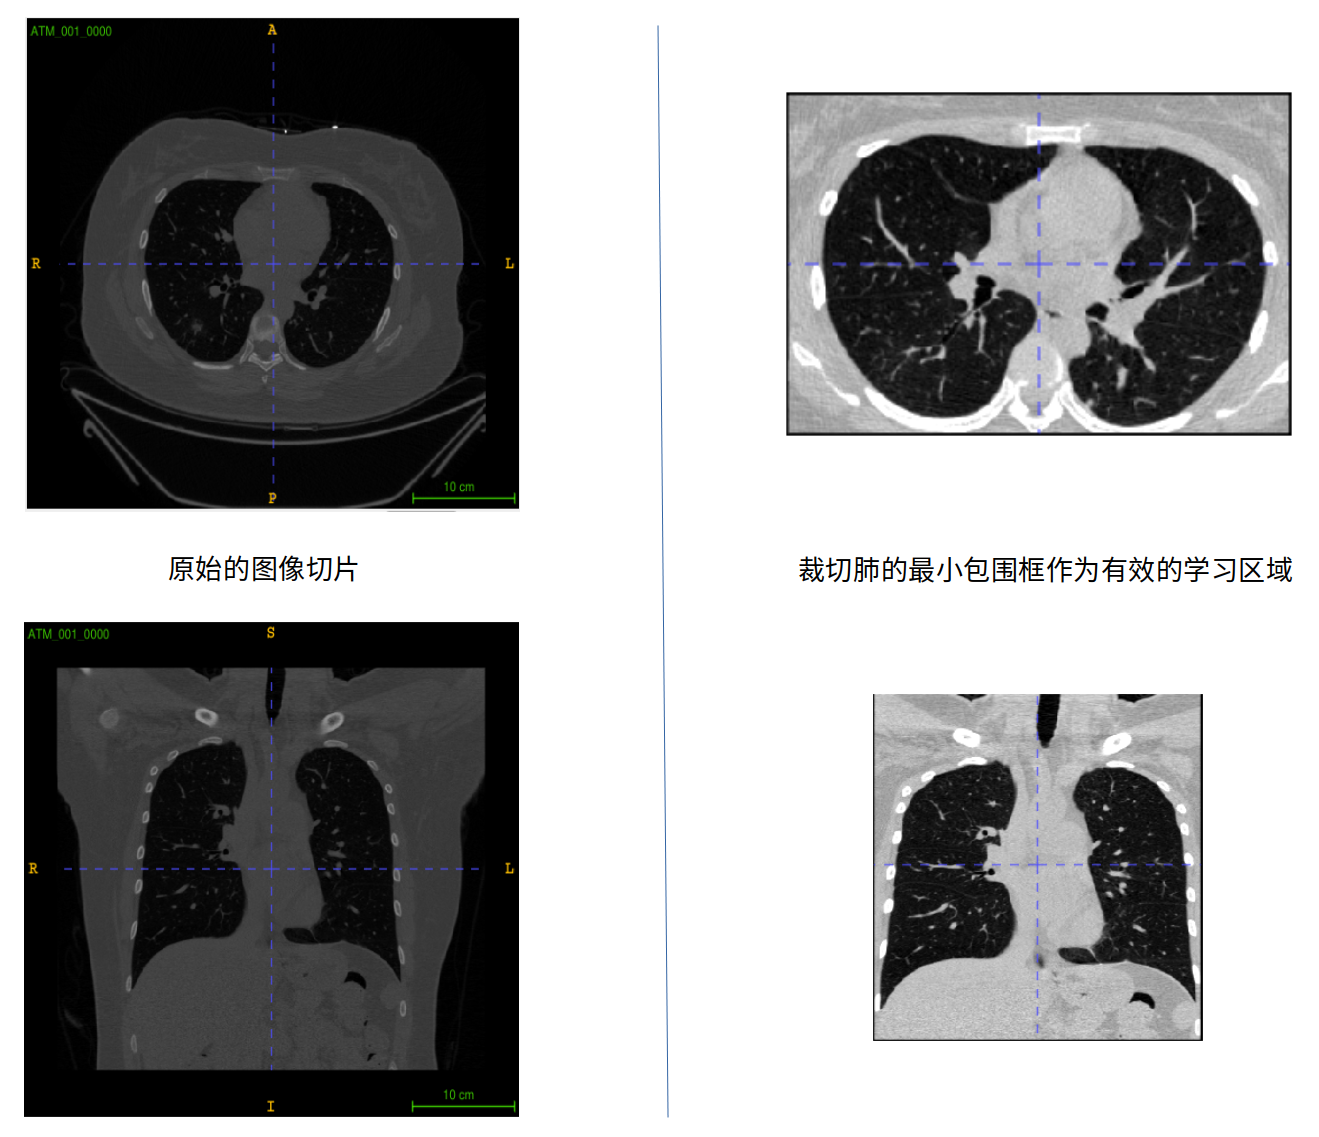
\includegraphics[width=0.7\textwidth]{image_crop}
    \caption{裁切CT图像切片的效果对比}
    \label{fig:cropimage}
\end{figure}
裁切后不仅可以减少计算量,最重要的是排除无关区域对网络的权重与偏置参数产生影响。

经过上述的裁切后,CT图像体的体积大幅缩小,就拿图\ref{fig:cropimage}的ATM-001-0000病例来说,CT图像体从
$D679 \times H512 \times W512$缩减到$D595 \times H225 \times W333$。但即使如此,对于单个GPU单元显存来说仍然比较大,
为此,我们将CT图像体切割成$D80 \times H192 \times W304$尺寸的长方体子块。本文使用由上海交通大学高性能计算中心提供的AI超算平台
来进行训练与计算的。AI超算的显卡型号为NVIDIA Tesla V100,切割成这样的长方体子块最大化利用了GPU的资源又不至于撑爆,可以
允许调整Batch size。本文的网络在训练时分别使用了1/2/4/8四种不同的Batch size, 经测试验证$D80 \times H192 \times W304$
的长方体子块在GPU显存中均运行良好。我们对训练集、验证集和测试集的CT图像体采用了如此相同的切割方法和尺寸。当然,你可能根据你的
GPU显存资源决定切割的长方体子块的大小,显存资源比较大则可以选择切割成更大的长方体子块。我们对CT图像体采用滑动窗口的切割方式,
在训练阶段滑动窗口的大小为$D64 \times H96 \times W152$,在验证和测试阶段则的滑动窗口大小为$D64 \times H72 \times W72$.
滑动窗口的意思是每次切割之前沿着宽度W、高度H、深度D方向逐次移动指定的距离。

为了增强训练效果,也是为了大幅扩大数据量,我们对每个切割的长方体子块图像块进行了数据增强,具体的数据增强方式有:
\begin{enumerate}\label{enum:data_augmentation}
    \item {\heiti 沿深度、高度、宽度三个轴随机翻转 RandomFlip}
    \item {\heiti 随机仿射变换并重采样 RandomAffine}
    \item {\heiti 随机高斯滤镜模糊图像 RandomBlur}
    \item {\heiti 给图像添加随机高斯噪声 RandomNoise}
    \item {\heiti 随机运动模糊,使图像产生运动伪影 RandomMotion}
    \item {\heiti 添加随机偏差场伪影 RandomBiasField}
    \item {\heiti 添加随机spike伪影,在图像空间产生不同方向的条纹 RandomSpike}
    \item {\heiti 添加随机残影 RandomGhosting}
\end{enumerate}
以上数据增强方式,我们通过组合不同的增强方式来联合增强切割的长方体子块图像数据。我们还加入随机概率作用于这些数据增强方式,
进一步增强图像数据。


\section{评价指标和分割效果可视化}
对于支气管气道树的分割任务,其目标是分割出精确的支气管三维模型,用于临床辅助诊疗。评价支气管气道树分割质量的好坏,有如下指标:
\begin{enumerate}
    \item 假阳性率 False Positive Rate, FPR
    
    假阳性代表着误检,也就是说将本不是支气管的体素错误地判定为支气管体素。假阳性率越高表示错误检查发生越多,分割结果愈不可信。
    
    \item 假阴性率 False Negative Rate, FNR
    
    假阴性代表着漏检,就是将本来是真实的支气管体素漏掉了,而认为是普通的背景体素。假阴性过高会导致临床诊断时可能将潜藏的真实
    疾病漏诊,而贻误了治疗时机。
    
    \item 灵敏度 Sensitivity
    
    灵敏度也叫真阳性率(True Positive Rate, TPR),其表示检测出来的真实支气管体素占实际的全部支气管体素的比例。 
    
    \item 精度 Precision
    
    精度表示检测出来的真实支气管体素跟真实的支气管体素与发生误检的假阳性支气管体素之和的比例,精度代表着模型的分割能力。在
    95\%的置信区间内,模型能辨识出实际的真实支气管体素的能力。精度越高,表示分割出来的支气管气道树越接近患者的真实情况,就能
    更可靠地帮助临床医生做出准确的病情诊断。
    
    \item 骰子相似度系数 Dice Similarity Coefficient, DSC
    
    DSC用来衡量网络分割的结果与金标准之间的相似性,是一种集合相似度度量函数。表示为预测的支气管体素与真实的支气管体素的交集
    跟预测的支气管体素加上真实的支气管体素进行比较。
    
    \item 检测到的分支 Branch Detected, BD
    
    BD表示模型检测到的分支数相比于参考的实际存在的分支总数
    
    \item 检测到的树长 Tree Length Detected, TLD
    
    树长为模型检测到的所有分支的中心线长度之和,TLD表示检测到的树长相比于参考的真实的树长。
\end{enumerate}
上述这些评价指标是在EXACT'09\cite{Lo2012ExtractionOA}上被提出,并被普遍接受和广泛使用的评价指标。评估的重点是放在提取
最完整的气道树,进入更高代的气道\footnote{注:在医学上通常使用代来表示支气管分支的相对关系。从咽喉部一直到肺部气管第一个分岔
前的气管称为第0代气管,从第一个分岔出来的左右肺主气管称为第1代气管,然后分岔到上/中/下肺叶的气管称为第2代气管,再分岔到段支气管
的称为第3代气管。如此类推,每分岔一个支气管,气管的代就增加1。气管的代越高,表示气管管腔直径就越细小。}并提取尽可能多的分支。

如何计算这些评价指标,我们以模型预测的支气管体素对比真实的支气管体素的比对表\ref{tbl:metrics_calculation}来说明,
并定义计算方法。
\begin{table}[!htp]
    \bicaption[评价指标计算方法说明]{评价指标计算方法说明}{The explanation of metrics calculation}
    \label{tbl:metrics_calculation}
    \centering
    \begin{tabular}{c|c|c|c|c}
        \hline
        \makecell{模型预测的支\\气管体素} & \makecell{真实的支气\\管体素} & \makecell{表示}  & 体素个数 
        & \makecell{在ITK-SNAP中\cite{Yushkevich2006ITKSNAP}的\\颜色标记} \\
        \hline
        1  &  0  & 假阳性 & ${Voxel}_{FP}$ & \textcolor{green}{绿色} \\
        \hline
        1  &  1  & 真阳性 & ${Voxel}_{TP}$ & \textcolor{blue}{蓝色} \\
        \hline
        0  &  0  & 真阴性 & ${Voxel}_{TN}$ & \textcolor{black}{黑色(背景)} \\
        \hline
        0  &  1  & 假阴性 & ${Voxel}_{FN}$ & \textcolor{red}{红色} \\
        \hline
    \end{tabular}
\end{table}
依据表\ref{tbl:metrics_calculation},上述的指标按如下的公式计算:
\begin{enumerate}
    \item 假阳性率
    
    \begin{equation}
        FPR = \frac{{Voxel}_{FP}}{{Voxel}_{FP} + {Voxel}_{TN}} \times 100\%
    \end{equation}
    
    \item 假阴性率
    
    \begin{equation}
        FNR = \frac{{Voxel}_{FN}}{{Voxel}_{FN} + {Voxel}_{TP}} \times 100\%
    \end{equation}
    
    \item 灵敏度
    
    \begin{equation}
        Sensitivity = \frac{{Voxel}_{TP}}{{Voxel}_{TP} + {Voxel}_{FN}} \times 100\%
    \end{equation}
    
    \item 精度
    
    \begin{equation}
        Precision = \frac{{Voxel}_{TP}}{{Voxel}_{TP} + {Voxel}_{FP}} \times 100\%
    \end{equation}
    
    \item 骰子相似度系数
    
    \begin{equation}
        DSC = \frac{2 * {Voxel}_{TP}}{({Voxel}_{TP} + {Voxel}_{FN}) + ({Voxel}_{TP} + {Voxel}_{FP})} \times 100\%
    \end{equation}
    
    \item 检测到的分支
    
    \begin{equation}
        BD = \frac{{Branch}_{seg}}{{Branch}_{gt}} \times 100\%
    \end{equation}
    其中${Branch}_{seg}$表示分割结果中检测到的分支数, ${Branch}_{gt}$表示真实存在的分支总数
    
    \item 检测到的树长
    
    \begin{equation}
        TLD = \frac{{Len}_{seg}}{{Len}_{gt}} \times 100\%
    \end{equation}
    其中${Len}_{seg}$表示分割结果中检测到的所有分支的中心线长度之和,${Len}_{gt}$表示真实存在的所有分支的中心线长度之和。
\end{enumerate}

经过模型训练后分割出来的支气管气道树,我们可以将其导入到ITK-SNAP\cite{Yushkevich2006ITKSNAP}软件中显示分割效果。这里
我们选择ATM\_054\_0000这个病例来可视化支气管气道树分割3D模型(这是经过3D-UNet基准网络分割的结果),如图
\ref{fig:airway_tree_model}所示。
\begin{figure}[!htp]
    \centering
    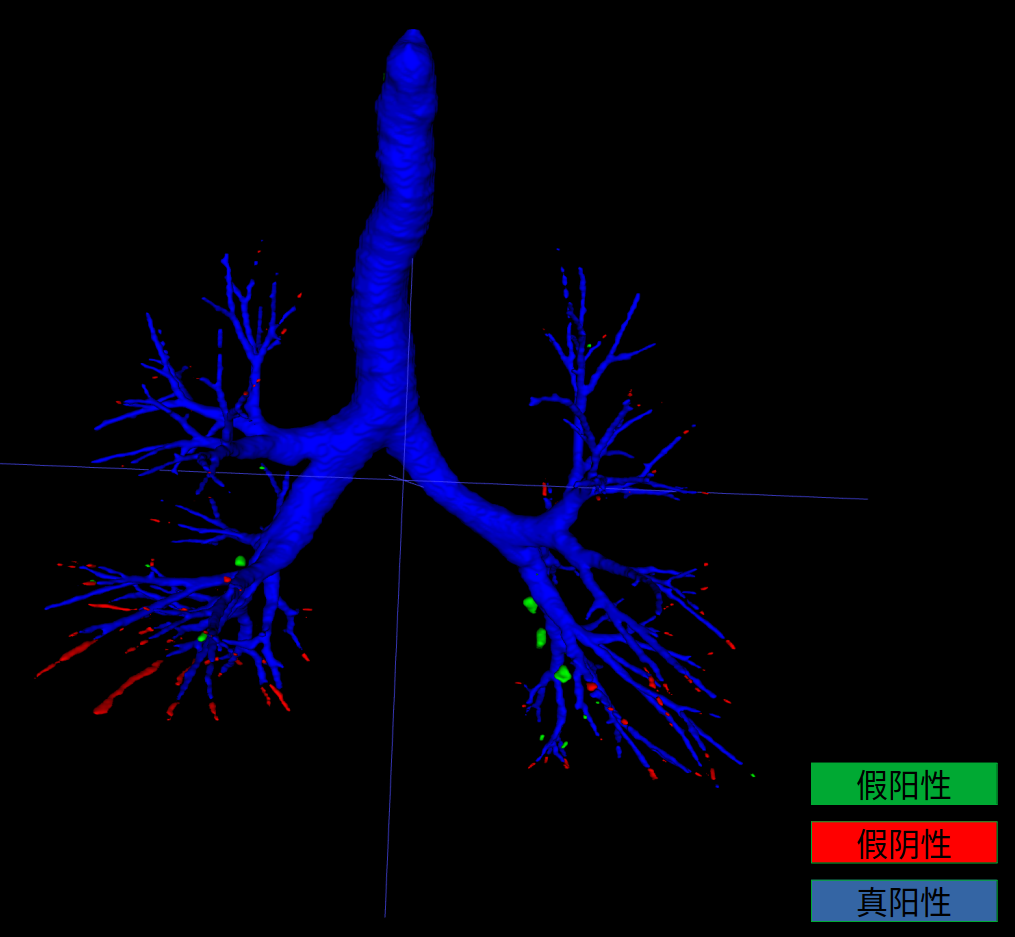
\includegraphics[width=0.8\textwidth]{visualize_colored_airway_tree}
    \bicaption[支气管气道树分割的3D模型]
        {支气管气道树分割的3D模型}
        {The 3D model of airway tree after segmentation}
    \label{fig:airway_tree_model}
\end{figure}
图例中\textcolor{green}{绿色}的表示\textcolor{green}{假阳性}体素,\textcolor{red}{红色}的表示\textcolor{red}{假阴性}
体素,\textcolor{blue}{蓝色}的表示\textcolor{blue}{真阳性}体素。

假阳性体素说明分割模型发生了误检,从图\ref{fig:airway_tree_model}可以明显看出绿色的体素跟气道树枝杆是分离的,不属于支气管
体素,而应该是黑色的背景体素,但3D-UNet分割模型却错误地认为是支气管体素。 假阴性说明分割模型发生了漏检,红色的体素原本是真实
存在的支气管,但3D-UNet分割模型漏掉了这些真实存在的支气管体素。这些漏掉的真实存在的支气管体素都是在支气管气道树的末端,是
属于非常细小的支气管,3D-UNet分割模型没有把这些细小的支气管体素分割出来,说明分割模型的能力还不够精细。最后,蓝色的体素则是
表明分割模型分割出来的支气管体素与真实存在的支气管体素是完全吻合的。粗大的气管、左右肺主支气管、上/中/下肺叶支气管和较细的段
支气管都被正确地分割出来,但在更细小的小叶支气管分割能力方面则显得还不够。

需要指出的,本中文对支气管气道树分割的颜色标记统一为绿色表示假阳性,红色表示假阴性,蓝色表示真阳性。全文保持一致的颜色标记,
后文中若没有特别指出颜色标记的意义,均视为与此处一致,不再重复地给出图例说明。

\section{实验结果与分析}
\subsection{3D-UNet基准网络训练过程}
我们将3D-UNet基准网络放在上海交通大学高性能计算中心的AI超级计算机上进行训练,输入是从ATM22数据集上随机挑选66例肺部CT扫描图像,按照
\ref{sec:ATM22}节介绍的裁切方法去掉无关的黑色背景区域,只保留肺部最小包围框作为有效学习区域。然后将这些经裁切的Cuboid体数据
按照$D64 \times H96 \times W152$的滑动窗口步长随机切割成$D80 \times H192 \times W304$的子块,每个子块都经过
\ref{enum:data_augmentation}节所述的8种数据增强方法进行增强。Label数据也是66例同病例的CT体数据,按照同样的方式进行
裁切和切割成$D80 \times H192 \times W304$的子块,但这些Label子块不进行数据增强。每一个图像Cuboid体数据子块与对应的
Label体数据子块绑定在一起。训练集、验证集和测试集的CT图像切割情况如表\ref{tbl:dataset_overview}所示。
\begin{table}[!htp]
    \bicaption[训练集、验证集和测试集的数据一览]{训练集、验证集和测试集的数据一览}
        {Overview of the cropped CT cube images among trainset, validateset and testset}
    \label{tbl:dataset_overview}
    \centering
    \begin{tabular}{c|c|c}
        \toprule
          & \makecell{CT扫描图像\\例数} & \makecell{切割成$D80 \times H192 \times W304$\\的子块总数} \\
        \midrule
        训练集 & 66 & 2202 \\
        验证集 & 9  & 415 \\
        测试集 & 19 & 770 \\
        \bottomrule 
    \end{tabular}
\end{table}
我们还会在将这些子块送给网络进行学习前会进行一次洗牌,完全打乱2202个子块的顺序,每一个迭代周期都会洗牌一次。同样地,我们也对
验证集的415个子块和测试集的770个子块在每个迭代周期都进行洗牌。

在训练过程中,我们使用TensorBoard收集每一个迭代周期Epoch的损失函数值,我们密切注视着损失函数的曲线。
我们观察到40多个迭代周期后,损失函数曲线已经平缓了,趋于收敛了,在60个迭代周期后我们便结束了训练过程。训练过程中的损失函数
曲线如图\ref{fig:lossfn_curve}所示。
\begin{figure}[!htp]
    \centering
    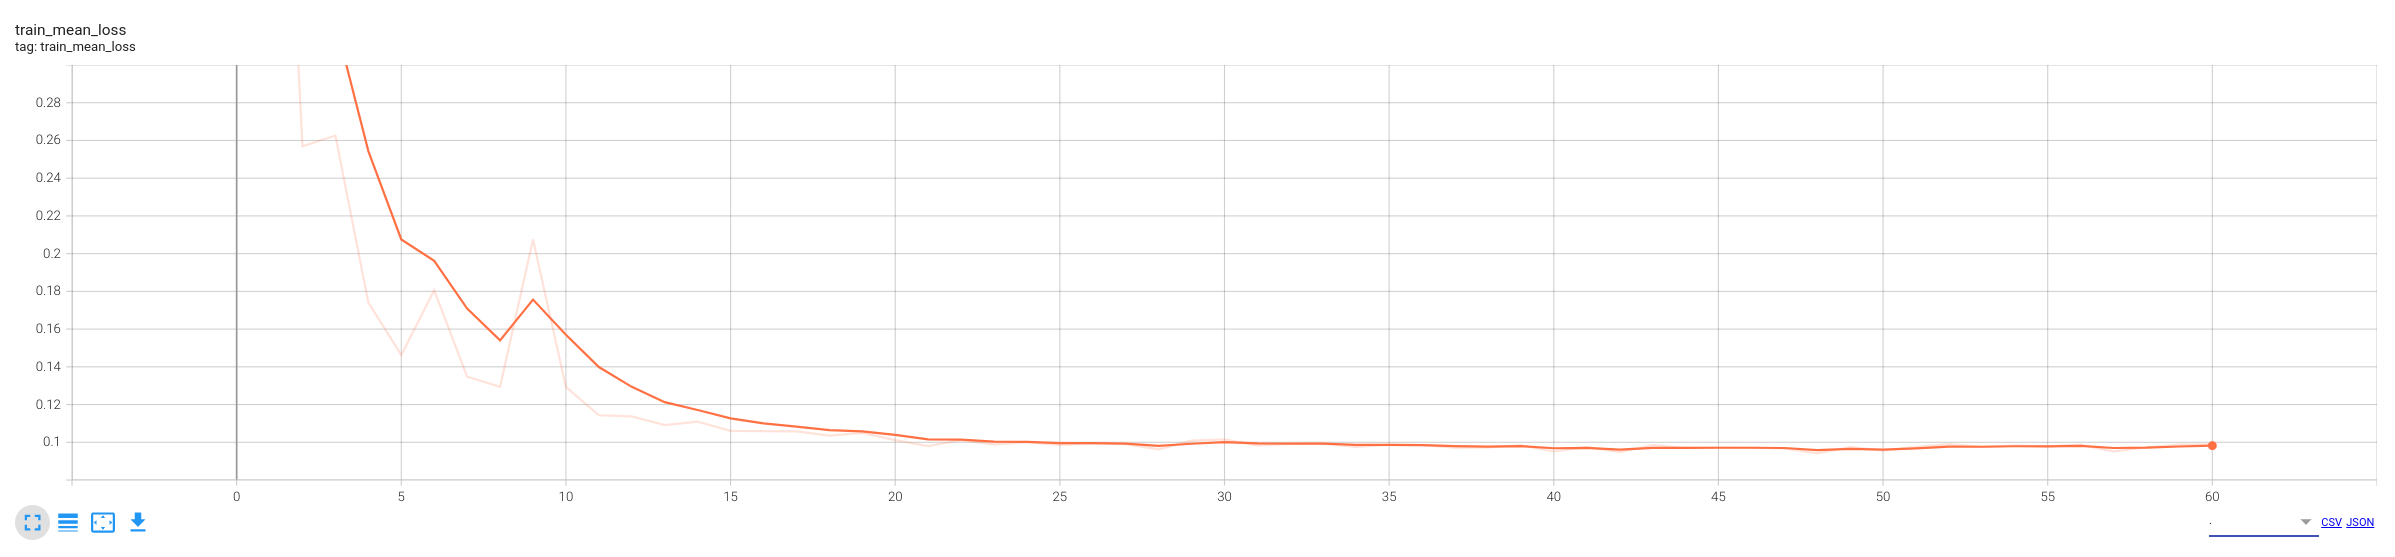
\includegraphics[width=\textwidth]{train_mean_loss_curve}
    \bicaption[3D-UNet基准网络训练时的损失函数曲线]
        {3D-UNet基准网络训练时的损失函数曲线}
        {The loss function curve of 3D-UNet baseline network during training process}
    \label{fig:lossfn_curve}
\end{figure}
在训练过程中,第一个迭代周期我们就对验证集的9例CT图像进行分割,输出每例CT图像的支气管气道树3D模型和指标数据。当然这个分割结果
肯定是非常糟糕的,但我们将它视为检验程序正确运行的参照物,训练迈出第一步的标志。之后每经过10个迭代周期,程序就会对验证集和测试集
里的CT图像进行分割,输出并保存每例CT图像的支气管气道树3D模型和指标数据。每5个迭代周期都会保存模型的Check Point状态和参数,
并以model\_epochnum.ckpt文件名(如第35个迭代周期的模型名字就是model\_035.ckpt)格式保存下来。这样可使我们能够在训练中断后
沿着上次的model\_xxx.ckpt继续训练,而不用浪费时间从头开始训练。训练完成后将模型Check Point状态和参数保存为model\_latest.ckpt,
作为后续验证过程和测试过程的预训练模型,直接加以使用。除了保存模型Check Point状态后参数外,我们在每10个迭代周期将指标数据
保存进TensorBoard。累积这些数据帮助我们观察网络的优化发展状况,分析这些数据帮助我们找到改进方向。

在验证过程中,我们直接使用预训练模型model\_latest.ckpt对验证集里的9例CT图像进行分割,输出每例CT图像的支气管气道树3D模型
和指标数据。在测试过程中,我们对测试集里的19例CT图像执行同样的操作。我们将在\ref{subsec:experiment_results}节展示这些
实验结果。

以上的训练、验证和测试过程均在一次提交的Slurm作业里完成。 3D-UNet基准网络使用了2张NVIDIA Tesla V100显卡,Batch-size
设置为4,即一次读入4个$D80 \times H192 \times W304$的子块,2202个子块需要551次循环才能算完,启动4个进程进行并行计算。
训练过程每个迭代周期平均耗时658.7秒,验证过程跟训练过程同样的设置,每迭代周期平均耗时4137.6秒,而测试过程每迭代周期平均耗时9309.6秒。
详细的运行时间见表\ref{tbl:time_consumption}。为什么每迭代周期验证耗时和测试耗时都明显比训练耗时要长得多? 这里需要解释一下。
验证过程需要对9例CT图像计算评价指标数据,还需要计算产生三维气道树模型。每计算一个三维气道树模型需要耗时6分钟之久,计算BD和TLD两个
指标也需要耗时5分钟左右。重要的是,计算三维气道树模型和BD、TLD指标数据无法使用GPU进行并行计算而加速,只能采用CPU串行计算方式。
这主要是三维气道树模型和BD、TLD指标的计算涉及到很多的逻辑判断,加之Python Numpy库函数没有GPU版本的,所以无法使用GPU加速计算。
\begin{table}[ht]
    \centering
    \bicaption[3D-UNet基准网络训练、验证、测试耗时一览表]
        {3D-UNet基准网络训练、验证、测试耗时一览表}
        {Time consumption of training, validating and testing on 3D-UNet baseline}
    \label{tbl:time_consumption}
    \scalebox{0.8}{
    \begin{tabular}{c|c|c|c||c|c|c|c}
        \hline
        \multicolumn{8}{c}{运行时间 (单位: 秒)} \\
        \hline
        \makecell{迭代\\周期} & \makecell{训练\\耗时} & \makecell{验证\\耗时} & \makecell{测试\\耗时} &
        \makecell{迭代\\周期} & \makecell{训练\\耗时} & \makecell{验证\\耗时} & \makecell{测试\\耗时} \\
        \hline
        1	& 745.56	& 5034.34	&          &   31	& 653.84	&           &         \\
        2	& 656.85	&           &          &   32	& 656.55	&           &         \\            	
        3	& 657.74	&           &          &   33	& 655.44	&           &         \\            	
        4	& 657.58	&           &          &   34	& 655.85	&           &         \\            	
        5	& 657.91	&           &          &   35	& 655.63	&           &         \\            	
        6	& 657.84	&           &          &   36	& 655.75	&           &         \\            	
        7	& 657.86	&           &          &   37	& 656.22	&           &         \\            	
        8	& 657.01	&           &          &   38	& 657.3		&           &         \\            	
        9	& 656.64	&           &          &   39	& 656.49	&           &         \\            	
        10	& 656.53	& 5068.17	& 9560.42  &   40	& 656.66	& 3770.93	& 9457.15 \\
        \hline
        11	& 663.29	&           &          &   41	& 654.77	&           &         \\             	
        12	& 656.7		&           &          &   42	& 656.61	&           &         \\             
        13	& 657.82	&           &          &   43	& 656.63	&           &         \\             	
        14	& 658.24	&           &          &   44	& 656.56	&           &         \\             	
        15	& 658.56	&           &          &   45	& 656.46	&           &         \\             	
        16	& 657.96	&           &          &   46	& 656.78	&           &         \\             	
        17	& 658.15	&           &          &   47	& 656.46	&           &         \\             	
        18	& 657.97	&           &          &   48	& 656.14	&           &         \\             	
        19	& 658.68	&           &          &   49	& 655.84	&           &         \\             	
        20	& 658.03	& 3770.34	& 9557.97  &   50	& 655.97	& 3770.28	& 8337.74 \\ 
        \hline
        21	& 660.52	&           &          &   51	& 656.05	&           &         \\  	
        22	& 656.01	&           &          &   52	& 655.59	&           &         \\  	
        23	& 656.75	&           &          &   53	& 655.69	&           &         \\  	
        24	& 655.99	&           &          &   54	& 656.75	&           &         \\  	
        25	& 656.48	&           &          &   55	& 657.62	&           &         \\  	
        26	& 659.39	&           &          &   56	& 657.26	&           &         \\  	
        27	& 658.22	&           &          &   57	& 658.17	&           &         \\  	
        28	& 659.65	&           &          &   58	& 658.94	&           &         \\  	
        29	& 658.81	&           &          &   59	& 657.99	&           &         \\  	
        30	& 658.45	& 3780.8	& 9544.24  &   60	& 658.28	& 3768.32	& 9399.98 \\ 	 	 	 	 	 	 	  	 	 	 	 	 	 	 	 	 	 	 	 	 	 	 	 	 	 	
        \hline
        61	&	        & 5252.09	&          &   62   &           &           & 9726.56 \\
        \hline
        \hline
        平均 & 658.7     & 4137.6    & 9309.6   & \multicolumn{2}{|c|}{总耗时} & \multicolumn{2}{|c}{38小时50分} \\
        \hline
    \end{tabular}
    }
\end{table}
验证集有9例CT图像,测试集有19例CT图像都需要计算指标数据和产生三维支气管气道树模型,所以每个迭代周期测试集计算耗时是验证集计算耗时
2倍多。 但好在我们不是每个迭代周期都会去计算验证集和测试集,而是每隔10个迭代周期才去计算一次。验证集在第一个迭代周期被计算一次,而
测试集并没有被计算。

表\ref{tbl:time_consumption}反映了我们的整个实验过程。经历了60个迭代周期训练过程完成。在第61个迭代周期,我们使用训练获得的最新模型
参数(即加载最新的预训练模型model\_latest.ckpt)来执行验证过程,第62个迭代周期执行测试过程。最后,3D-UNet基准网络训练、验证和测试全过程
总耗时38小时50分钟,完成一个完整实验。

\subsection{实验结果和分析}\label{subsec:experiment_results}
上述的训练、验证和测试过程完成后,我们来展示实验结果。由于篇幅的原因,我们挑选验证集里的9例CT图像,展示支气管气道树3D模型的
可视化效果和他们的指标数据。而对于测试集里的19例CT图像,19张支气管气道树3D模型图片实在太多放不下,我们只展示19组指标数据。

我们将进行横向和纵向的对比。
\begin{enumerate}
    \item[A.] 在横向对比时,我们对验证集的9例CT图像,每例CT图像均匀地取5张切片,选取中间的那张切片。排列这9张
切片看看它们的分割效果和指标数据,如表\ref{tbl:hcomparison_metrics}所示。

    \begin{table}[!htp]
        \bicaption[验证集CT切片图像分割效果与指标横向比较]
            {验证集CT切片图像分割效果与指标横向比较}
            {Horizontal comparison of segmentation and metrics in the validateset}
        \label{tbl:hcomparison_metrics}
        \centering
        \begin{tabular}{|c|c|c|}
            \hline
            ATM\_029\_0000 & ATM\_054\_0000 & ATM\_055\_0000 \\
            Slice \#296 & Slice \#264 & Slice \#229 \\
            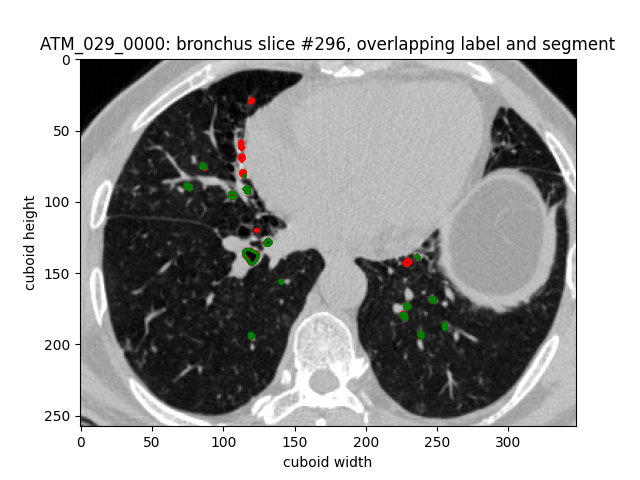
\includegraphics[width=0.3\textwidth]{results/baseline/val060/ATM_029_0000_bronchus_segmentation_slice296_at_val_epoch60} &
            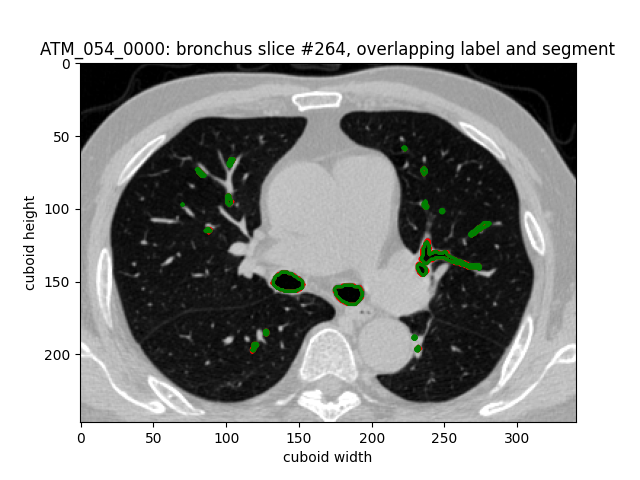
\includegraphics[width=0.3\textwidth]{results/baseline/val060/ATM_054_0000_bronchus_segmentation_slice264_at_val_epoch60} &
            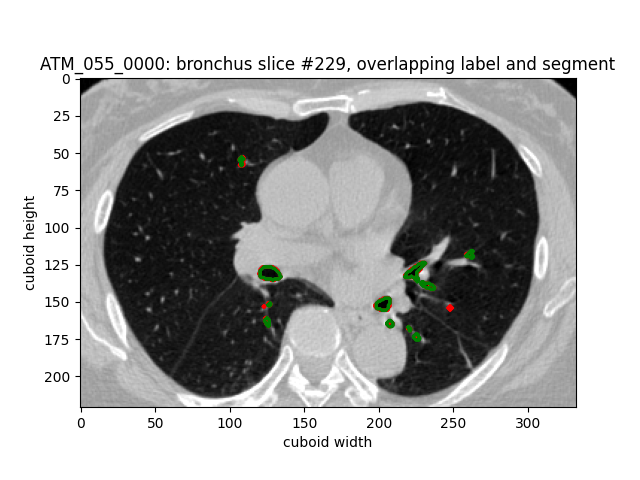
\includegraphics[width=0.3\textwidth]{results/baseline/val060/ATM_055_0000_bronchus_segmentation_slice229_at_val_epoch60} \\
            FPR = 0.066\%           & FPR = 0.068\%             & FPR = 0.056\% \\
            FNR = 14.286\%          & FNR = 5.991\%             & FNR = 9.966\% \\
            Sensitivity = 85.714\%  & Sensitivity = 94.009\%    & Sensitivity = 90.034\% \\
            Precision = 72.558\%    & Precision = 92.039\%      & Precision = 86.469\% \\
            DSC = 78.59\%           & DSC = 93.01\%             & DSC = 88.22\% \\
            \hline
            
            ATM\_057\_0000 & ATM\_091\_0000 & ATM\_174\_0000 \\
            Slice \#287 & Slice \#281 & Slice \#74 \\
            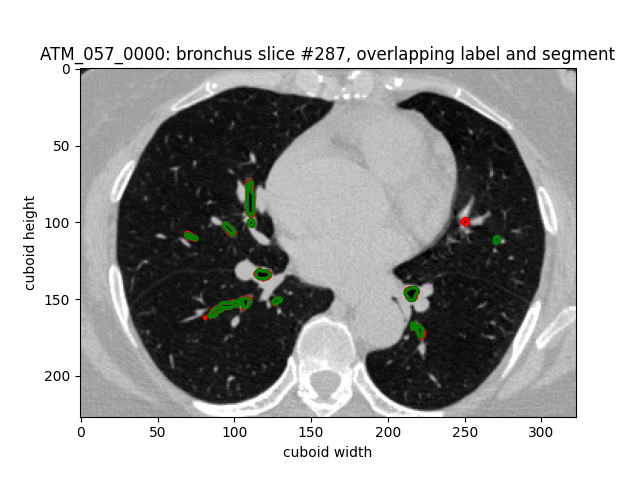
\includegraphics[width=0.3\textwidth]{results/baseline/val060/ATM_057_0000_bronchus_segmentation_slice287_at_val_epoch60} &
            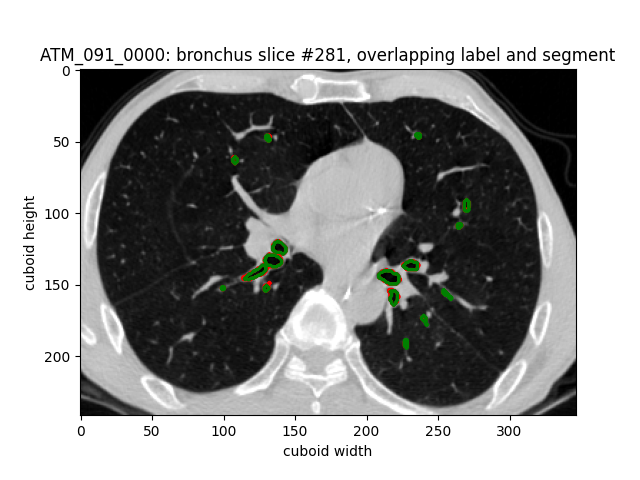
\includegraphics[width=0.3\textwidth]{results/baseline/val060/ATM_091_0000_bronchus_segmentation_slice281_at_val_epoch60} &
            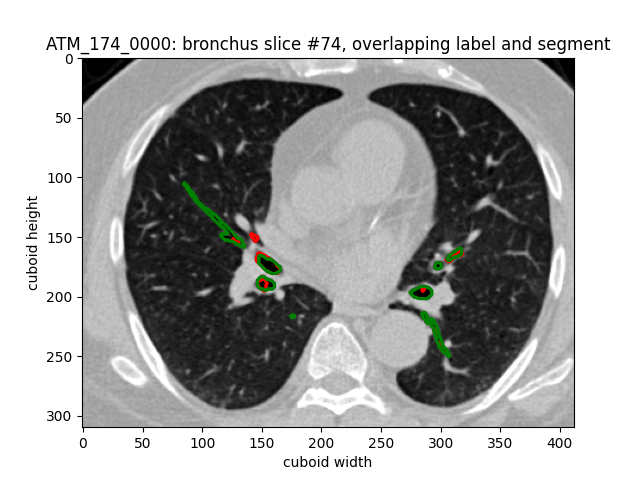
\includegraphics[width=0.3\textwidth]{results/baseline/val060/ATM_174_0000_bronchus_segmentation_slice74_at_val_epoch60} \\
            FPR = 0.089\%           & FPR = 0.068\%             & FPR = 0.044\% \\
            FNR = 5.06\%            & FNR = 3.419\%             & FNR = 69.159\% \\
            Sensitivity = 94.94\%   & Sensitivity = 96.581\%    & Sensitivity = 30.841\% \\
            Precision = 83.073\%    & Precision = 88.802\%      & Precision = 82.5\% \\
            DSC = 88.61\%           & DSC = 92.53\%             & DSC = 44.9\% \\
            \hline
            
            ATM\_215\_0000 & ATM\_505\_0000 & ATM\_688\_0000 \\
            Slice \#216 & Slice \#177 & Slice \#292 \\
            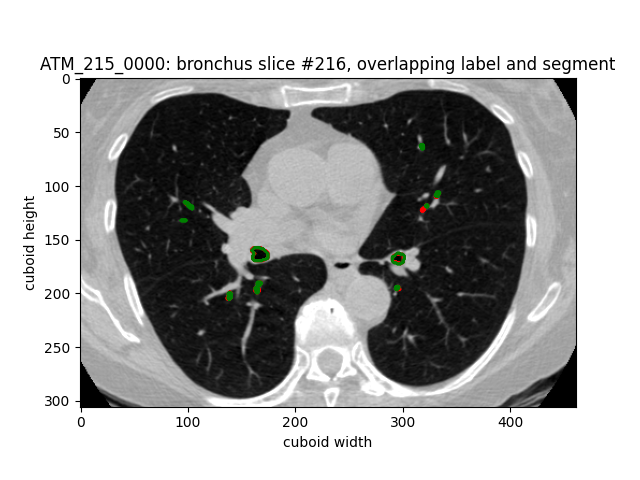
\includegraphics[width=0.3\textwidth]{results/baseline/val060/ATM_215_0000_bronchus_segmentation_slice216_at_val_epoch60} &
            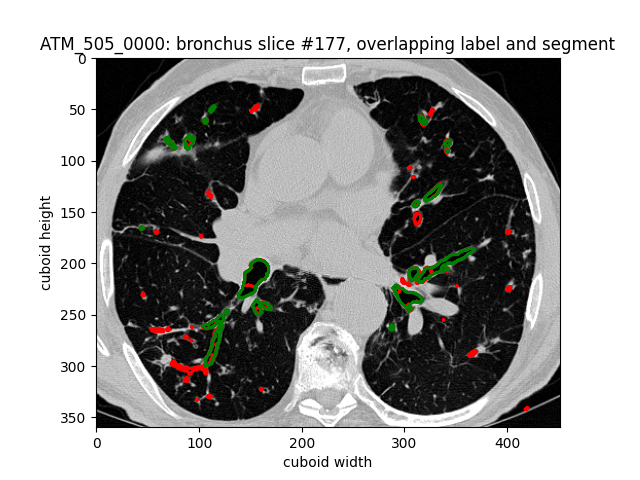
\includegraphics[width=0.3\textwidth]{results/baseline/val060/ATM_505_0000_bronchus_segmentation_slice177_at_val_epoch60} &
            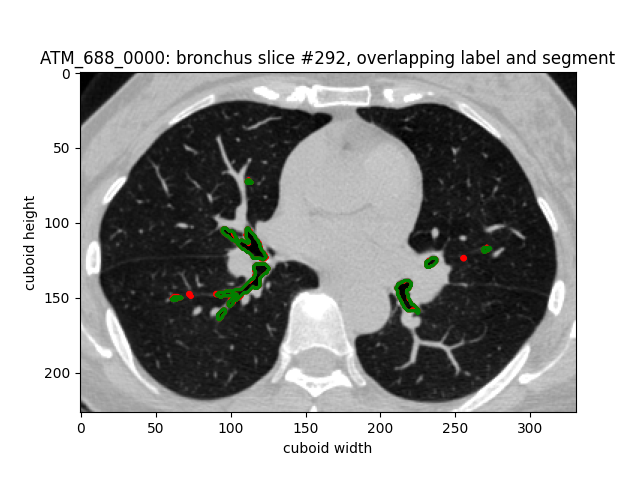
\includegraphics[width=0.3\textwidth]{results/baseline/val060/ATM_688_0000_bronchus_segmentation_slice292_at_val_epoch60} \\
            FPR = 0.021\%           & FPR = 0.026\%             & FPR = 0.05\% \\
            FNR = 18.069\%          & FNR = 44.246\%             & FNR = 2.038\% \\
            Sensitivity = 81.931\%  & Sensitivity = 55.754\%    & Sensitivity = 97.962\% \\
            Precision = 90.068\%    & Precision = 72.892\%      & Precision = 94.411\% \\
            DSC = 85.81\%           & DSC = 63.18\%             & DSC = 96.15\% \\
            \hline
        \end{tabular}
    \end{table}
    
    需要说明的是,表\ref{tbl:hcomparison_metrics}中的指标数据是基于当前切片计算的,不是基于整个气道树来计算的,因此就不
    带有BD和TLD两个指标的数据了。还有一点,切片图像中由绿色像素框起来的区域是真实的气管,红色的像素是分割出来的。绿色像素覆盖
    在红色像素上,对于没有覆盖住而露出来的红色像素是假阳性的。
    
    \item[B.] 在纵向对比时,我们挑选ATM\_054\_0000这个病例,将第10个迭代周期,第20/30/40/50/60个迭代周期里的Slice
    \#264拿出来对比,看看它们的分割效果和指标数据,如表\ref{tbl:vcomparison_metrics}所示。
    \begin{table}[ht]
        \bicaption[验证集ATM\_054\_0000病例第264张切片图像分割效果与指标纵向比较]
            {验证集ATM\_054\_0000病例第264张切片图像分割效果与指标纵向比较}
            {Vertical comparison of segmentation and metrics for ATM\_054\_0000 slice \#264}
        \label{tbl:vcomparison_metrics}
        \centering
        \begin{tabular}{|c|c|c|}
            \hline
            ATM\_054\_0000 & ATM\_054\_0000 & ATM\_054\_0000 \\
            Epoch \#10 & Epoch \#20 & Epoch \#30 \\
            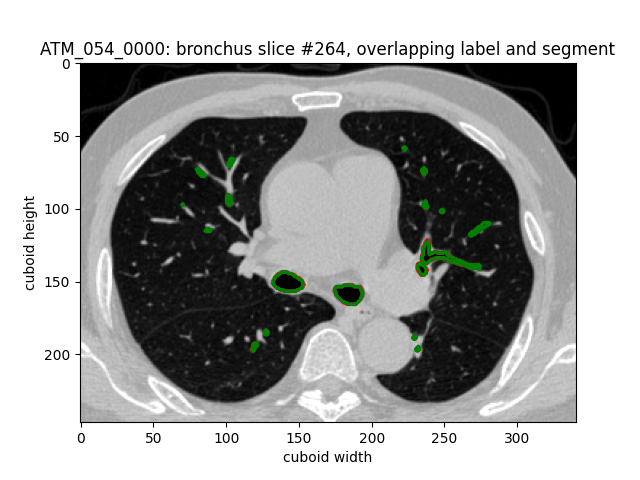
\includegraphics[width=0.3\textwidth]{results/baseline/val010/ATM_054_0000_bronchus_segmentation_slice264_at_val_epoch10} &
            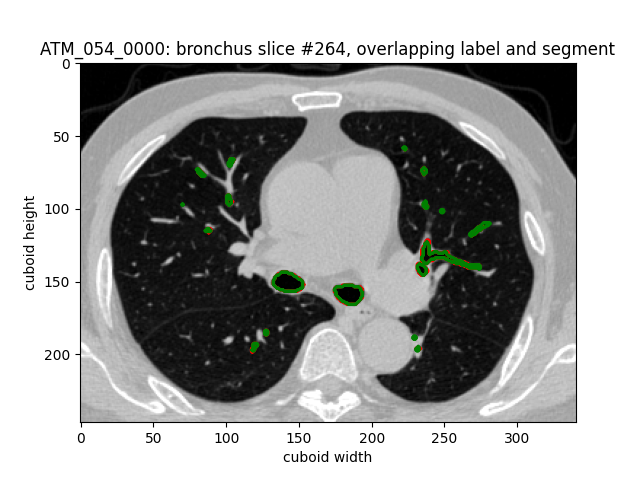
\includegraphics[width=0.3\textwidth]{results/baseline/val020/ATM_054_0000_bronchus_segmentation_slice264_at_val_epoch20} & 
            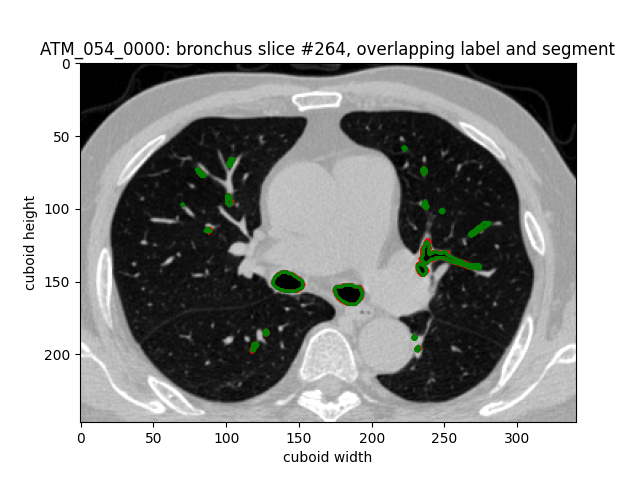
\includegraphics[width=0.3\textwidth]{results/baseline/val030/ATM_054_0000_bronchus_segmentation_slice264_at_val_epoch30} \\
            FPR = 0.025\%           & FPR = 0.061\%             & FPR = 0.066\% \\
            FNR = 12.268\%          & FNR = 6.419\%             & FNR = 6.419\% \\
            Sensitivity = 87.732\%  & Sensitivity = 93.581\%    & Sensitivity = 93.581\% \\
            Precision = 96.698\%    & Precision = 92.786\%      & Precision = 92.264\% \\
            DSC = 92.0\%            & DSC = 93.18\%             & DSC = 92.92\% \\
            \hline
            ATM\_054\_0000 & ATM\_054\_0000 & ATM\_054\_0000 \\
            Epoch \#40 & Epoch \#50 & Epoch \#60 \\
            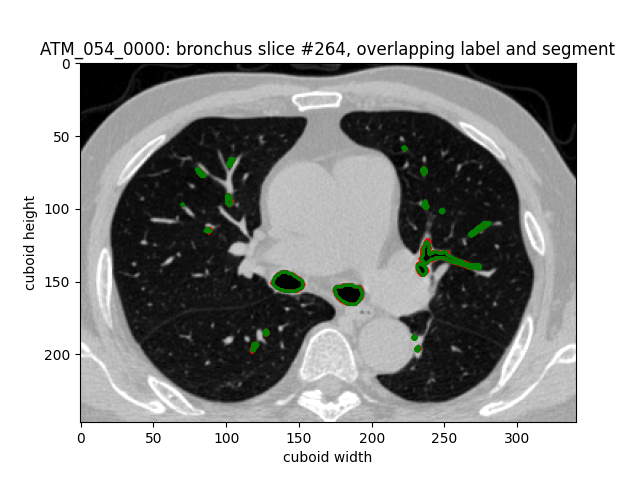
\includegraphics[width=0.3\textwidth]{results/baseline/val040/ATM_054_0000_bronchus_segmentation_slice264_at_val_epoch40} &
            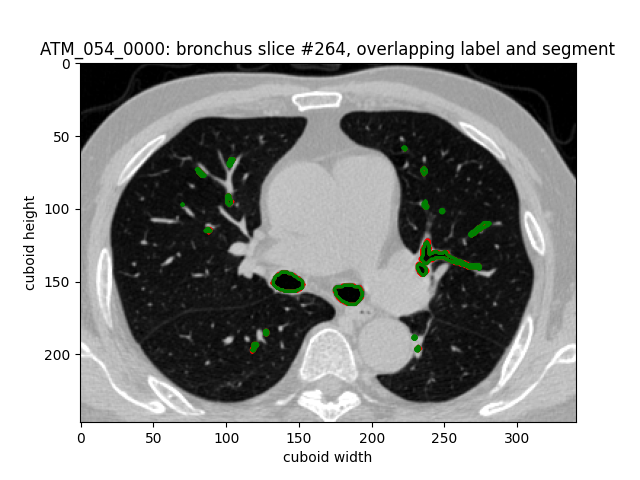
\includegraphics[width=0.3\textwidth]{results/baseline/val050/ATM_054_0000_bronchus_segmentation_slice264_at_val_epoch50} & 
            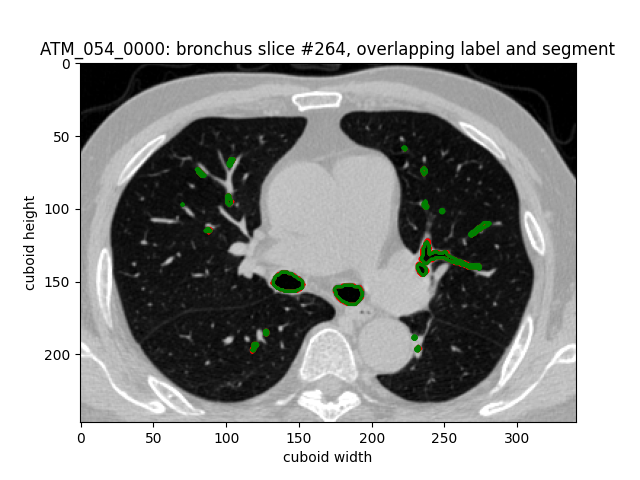
\includegraphics[width=0.3\textwidth]{results/baseline/val060/ATM_054_0000_bronchus_segmentation_slice264_at_val_epoch60} \\
            FPR = 0.066\%          & FPR = 0.068\%             & FPR = 0.068\% \\
            FNR = 6.277\%          & FNR = 6.277\%             & FNR = 5.991\% \\
            Sensitivity = 93.723\% & Sensitivity = 93.723\%    & Sensitivity = 94.009\% \\
            Precision = 92.275\%   & Precision = 92.017\%      & Precision = 92.039\% \\
            DSC = 92.99\%          & DSC = 92.86\%             & DSC = 93.01\% \\
            \hline
        \end{tabular}
    \end{table}

\end{enumerate}

从表\ref{tbl:hcomparison_metrics}看,ATM\_174\_0000 Slice \#74的Sensitivity和DSC两项指标表现得最差,这是因为
该CT图像的切片数量最少,其支气管气道明显狭窄,可能患有肺部疾病。倒数第二差的是ATM\_505\_0000 Slice \#177这张切片,存在
很多红色的像素表明假阴性像素很多,它们通常是一些比较细小的支气管。分割网络遗漏掉了这些真实存在的支气管体素。在这9例CT切片图像
中分割最好的当属于ATM\_688\_0000 Slice \#292, Sensitivity, Precision, DSC分别取得了97.62\%, 94.411\%, 96.15\%
的高分。这表明分割网络对于肺叶支气管、段支气管这种中等管腔直径的支气管能很清晰地分割出来。

从表\ref{tbl:vcomparison_metrics}看,随着训练的持续进行,从第20个迭代周期开始,分割性能就逐渐开始稳定下来。Sensitivity,
Precision和DSC都已经达到了92\%以上的优秀表现。不管是对于左右肺主气管、肺叶支气管,还是很细小的段支气管都可能清晰地分割出来,
证明3D-UNet基准网络性能基本上能达到临床应用的水平。

最后我们来看看3D-UNet网络对整个支气管气道树的分割表现。对于测试集的19例CT图像的分割,其性能指标如表
\ref{tbl:testset_airway_tree_metrics}所示。其中打下划线强调的表示在当前指标表现最出色的。
\begin{table}[ht]
    \bicaption[测试集上3D-UNet基准网络对支气管气道树分割的性能指标表现]
        {测试集上3D-UNet基准网络对支气管气道树分割的性能指标表现}
        {The metrics table of 3D-UNet baseline model segmenting airway tree in testset}
    \label{tbl:testset_airway_tree_metrics}
    \centering
    \begin{tabular}{cccccccc}
        \toprule
        病例名称          & FPR           & FNR            & Sensitivity     & Precision      & DSC           & BD            & TLD           \\
        \midrule
        ATM\_001\_0000 & \uline{0.006} & 7.24           & 92.76           & \uline{98.089} & 95.35         & 68.95         & 84.17         \\
        ATM\_024\_0000 & 0.031         & 7.236          & 92.764          & 90.916         & 91.83         & 84.18         & 92.86         \\
        ATM\_034\_0000 & 0.022         & 3.705          & 96.295          & 96.251         & 96.27         & 90.75         & 93.93         \\
        ATM\_041\_0000 & 0.047         & 4.808          & 95.192          & 87.189         & 91.02         & 82.38         & 90.38         \\
        ATM\_060\_0000 & 0.024         & 2.534          & 97.466          & 93.12          & 95.24         & 88.03         & 92.72         \\
        ATM\_061\_0000 & 0.028         & 3.121          & 96.879          & 91.897         & 94.32         & 86.15         & 90.8          \\
        ATM\_074\_0000 & 0.053         & 3.838          & 96.162          & 87.038         & 91.37         & 80.49         & 89.86         \\
        ATM\_075\_0000 & 0.023         & 4.633          & 95.367          & 93.65          & 94.5          & 81.13         & 88.56         \\
        ATM\_080\_0000 & 0.026         & 4.067          & 95.933          & 93.183         & 94.54         & 76.9          & 88.11         \\
        ATM\_150\_0000 & 0.082         & 3.902          & 96.098          & 80.036         & 87.33         & 72.12         & 87.62         \\
        ATM\_158\_0000 & 0.044         & 3.461          & 96.539          & 86.953         & 91.5          & 80.75         & 90.48         \\
        ATM\_163\_0000 & 0.035         & 4.301          & 95.699          & 91.958         & 93.79         & 83.23         & 91.34         \\
        ATM\_197\_0000 & 0.032         & 9.234          & 90.766          & 90.81          & 90.79         & 59.71         & 78.46         \\
        ATM\_245\_0000 & 0.038         & \uline{0.309}  & \uline{99.691}  & 83.496         & 90.88         & \uline{100}   & \uline{100}   \\
        ATM\_246\_0000 & 0.04          & 0.611          & 99.389          & 82.853         & 90.37         & \uline{100}   & \uline{100}   \\
        ATM\_260\_0000 & 0.016         & 1.041          & 98.959          & 94.227         & \uline{96.53} & 98.34         & 97.93         \\
        ATM\_266\_0000 & 0.019         & 2.351          & 97.649          & 93.112         & 95.33         & 99.38         & 98.39         \\
        ATM\_271\_0000 & 0.049         & 1.044          & 98.956          & 86.544         & 92.33         & 97.6          & 97.62         \\
        ATM\_638\_0000 & 0.014         & 3.152          & 96.848          & 95.199         & 96.02         & 90.48         & 95.45         \\
        \bottomrule
    \end{tabular}
\end{table}
从表\ref{tbl:testset_airway_tree_metrics}可以看出,ATM\_245\_0000这一例CT图像分割表现最好,BD和TLD两个指标竟然
达到例100\%, 这说明已经将支气管气道树中的分支全部检测出来,也获得了最长的分支中心线长度之和。

对于验证集的9例CT图像,我们不仅要展示支气管气道树分割的可视化结果,如表\ref{tbl:visualize_airway_3d_model}所示。
\begin{table}[!htp]
    \bicaption[验证集9例CT图像的支气管气道树分割可视化3D模型]
        {验证集9例CT图像的支气管气道树分割可视化3D模型}
        {Visualize the airway 3D model of 9 CT cases in validateset}
    \label{tbl:visualize_airway_3d_model}
    \centering
    \begin{tabular}{|c|c|c|}
        \hline
        ATM\_029\_0000 & ATM\_054\_0000 & ATM\_055\_0000 \\
        \hline
        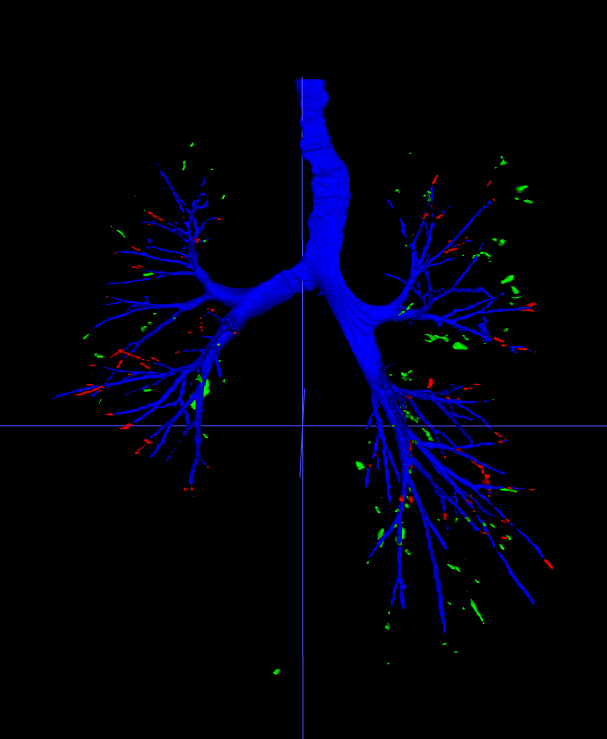
\includegraphics[width=0.3\textwidth]{results/baseline/validate/ATM_029_0000_airway_tree_with_3colors_at_val_epoch1} &
        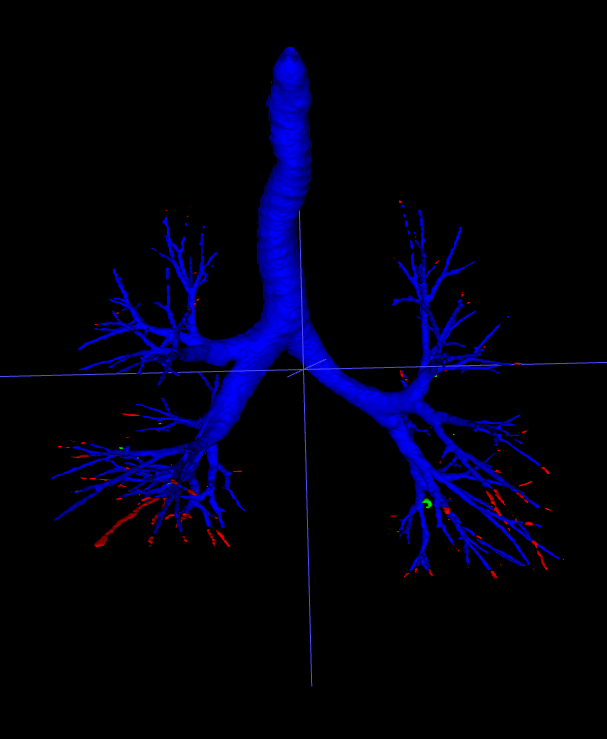
\includegraphics[width=0.3\textwidth]{results/baseline/validate/ATM_054_0000_airway_tree_with_3colors_at_val_epoch1} &
        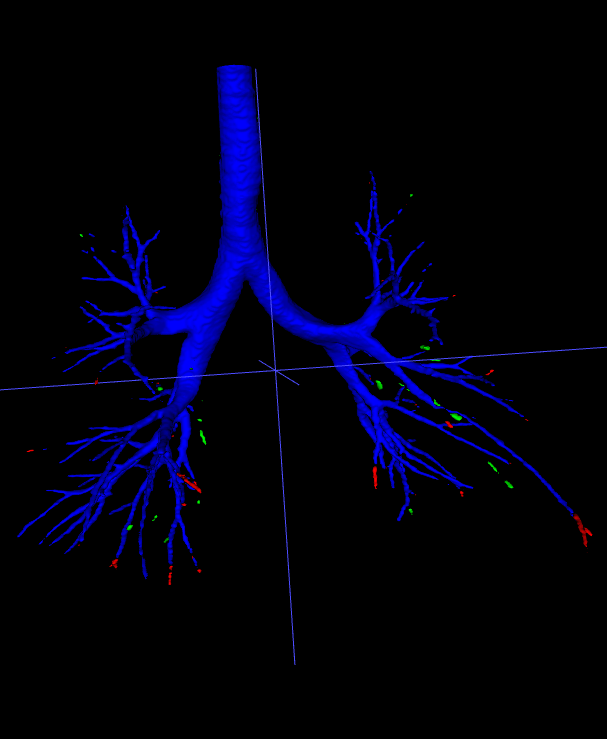
\includegraphics[width=0.3\textwidth]{results/baseline/validate/ATM_055_0000_airway_tree_with_3colors_at_val_epoch1} \\
        \hline
        ATM\_057\_0000 & ATM\_091\_0000 & ATM\_174\_0000 \\
        \hline
        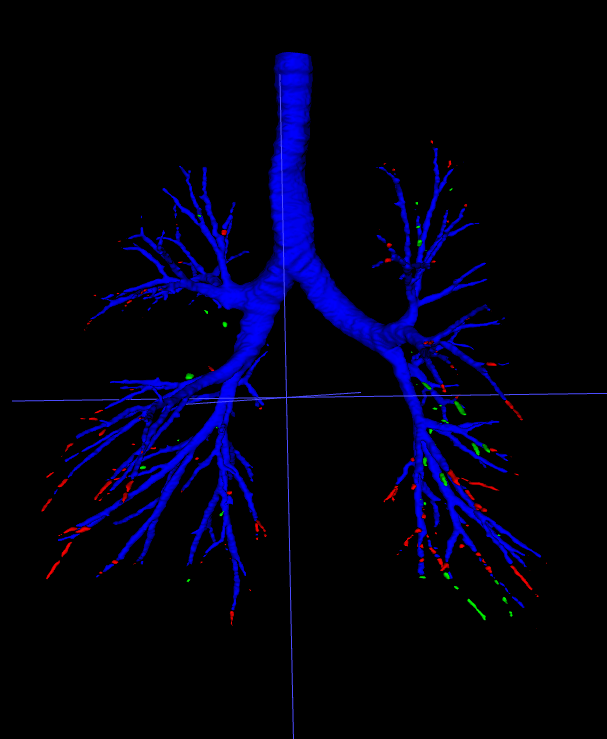
\includegraphics[width=0.3\textwidth]{results/baseline/validate/ATM_057_0000_airway_tree_with_3colors_at_val_epoch1} &
        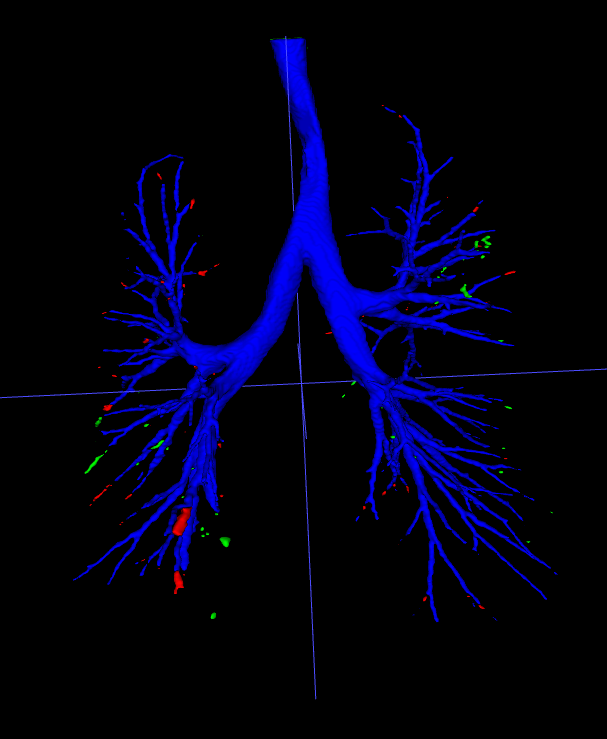
\includegraphics[width=0.3\textwidth]{results/baseline/validate/ATM_091_0000_airway_tree_with_3colors_at_val_epoch1} &
        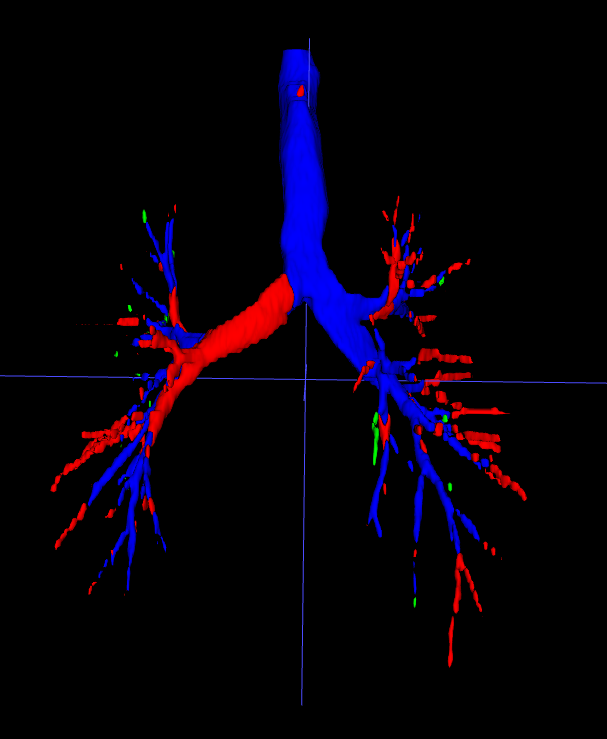
\includegraphics[width=0.3\textwidth]{results/baseline/validate/ATM_174_0000_airway_tree_with_3colors_at_val_epoch1} \\
        \hline
        ATM\_215\_0000 & ATM\_505\_0000 & ATM\_688\_0000 \\
        \hline
        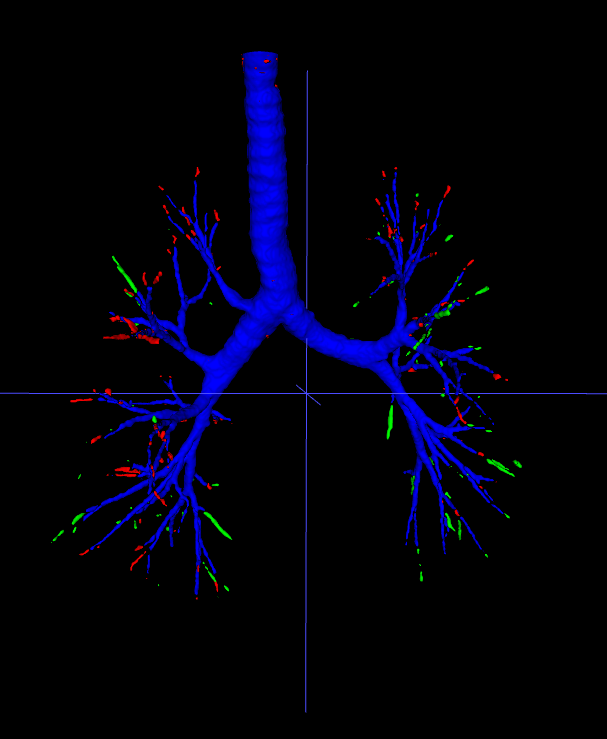
\includegraphics[width=0.3\textwidth]{results/baseline/validate/ATM_215_0000_airway_tree_with_3colors_at_val_epoch1} &
        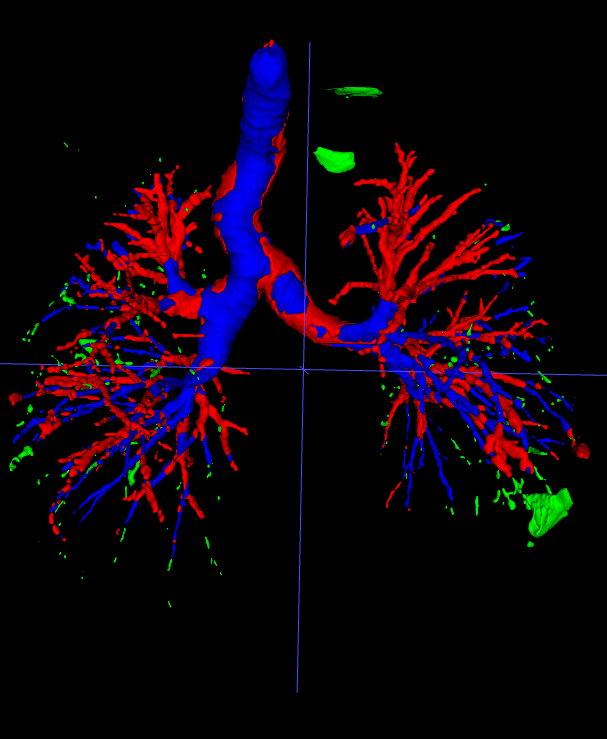
\includegraphics[width=0.3\textwidth]{results/baseline/validate/ATM_505_0000_airway_tree_with_3colors_at_val_epoch1} &
        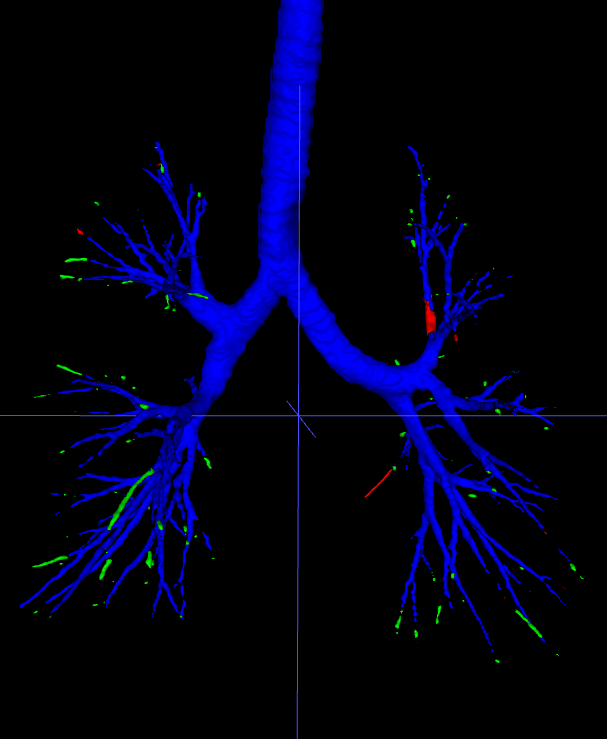
\includegraphics[width=0.3\textwidth]{results/baseline/validate/ATM_688_0000_airway_tree_with_3colors_at_val_epoch1} \\
        \hline
    \end{tabular}
\end{table}
还有完整的指标数据,见表\ref{tbl:validateset_airway_tree_metrics}。
\begin{table}[!htp]
    \bicaption[验证集9例CT图像的支气管气道树分割指标]
        {验证集9例CT图像的支气管气道树分割指标}
        {The segmentation metrics of 9 CT cases in validateset}
    \centering
    \label{tbl:validateset_airway_tree_metrics}
\begin{tabular}{cccccccc}
        \toprule
        病例名称          & FPR           & FNR            & Sensitivity     & Precision      & DSC           & BD            & TLD           \\
        \midrule
        ATM\_029\_0000 & 0.017           & 9.222          & 90.778          & 93.232         & 91.99         & 80.34         & 88.48         \\
        ATM\_054\_0000 & 0.032           & 3.876          & 96.124          & 93.343         & 94.71         & 76.78         & 85.61         \\
        ATM\_055\_0000 & 0.031           & 3.571          & 96.429          & 91.66          & 93.98         & 82.51         & 89.9          \\
        ATM\_057\_0000 & 0.03            & 5.757          & 94.243          & 92.35          & 93.29         & 72.85         & 84.36         \\
        ATM\_091\_0000 & 0.034           & 3.432          & 96.568          & 91.148         & 93.78         & 84.04         & 91.09         \\
        ATM\_174\_0000 & 0.019           & 26.864         & 73.136          & 94.026         & 82.28         & \colorbox{red}{32.38}         & \colorbox{red}{47.19}         \\
        ATM\_215\_0000 & 0.023           & 9.419          & 90.581          & 91.951         & 91.26         & 73.3          & 84.83         \\
        ATM\_505\_0000 & 0.05            & 55.899         & 44.101          & 84.808         & 58.03         & \colorbox{red}{21.5}          & \colorbox{red}{39.1}          \\
        ATM\_688\_0000 & 0.023           & 2.217          & 97.783          & 93.409         & 95.55         & 93.07         & 95.73         \\
        \bottomrule
    \end{tabular}
\end{table}
在表\ref{tbl:visualize_airway_3d_model}中我们看到ATM\_174\_0000和ATM\_505\_0000两个病例中出现大量的红色的假阴性
体素。结合表\ref{tbl:validateset_airway_tree_metrics}中这两个病例的BD、TLD两项指标低至30\%的不正常现象\footnote{
表\ref{tbl:validateset_airway_tree_metrics}中红色标记的数据},而Precision
能够达到90\%以上。纵览这9张气道树3D分割图,其他7张图都没有在气管、左右肺主气管发生漏检。 
所以,我们推断ATM\_174\_0000和ATM\_505\_0000两个病例的支气管气道树异常的原因可能是:
\begin{enumerate}
    \item[a)] 图像异位,做标注工作的临床医生没有看到明确的支气管管壁边缘而没有标注;
    \item[b)] 患者有严重的肺部疾病,支气管管壁破裂或缺失。
\end{enumerate}
我们更倾向于后者。

在此需要强调一点,我们是将3D-UNet作为我们的基准网络,所以在此没有做消融研究Ablation Study,没有凸显3D-UNet网络比其他
已知网络更优秀。从上述的实验结果展示和分析,我们认识到3D-UNet网络存在不足之处,后面的章节以3D-UNet网络为基础,在此之上进行
改进。

\section{本章小结}

本章详细讲述了3D-UNet这一基准网络,我们在基于CT扫描图像的支气管气道树分割任务中采用3D-UNet网络来对肺部支气管进行分割,我们
使用Python语言与PyTorch深度学习框架设计实现了一个3D-UNet分割网络,针对ATM22数据集进行特定的优化设计。我们在上海交通大学
高性能计算中心的AI超算上训练网络,训练完成后在验证集和测试集上输出完整的支气管气道树三维模型和评价指标数据。我们展示了实验结果,
可视化显示支气管气道树的3D模型,分析这些实验数据,并对两个明显异常的病例进行分析推断异常的产生原因。

通过以上实验证明了3D-UNet网络可以胜任三维支气管气道树的分割任务,但在精度准确率、FPR和DSC等指标方面还不够,需要进一步改进3D-UNet
网络。后文在此实验的基础上研究如何改进该网络,以更好更精确地分割支气管气道树三维模型。

% !TEX root = ../main.tex

\chapter{数学与引用文献的标注}

\section{数学}

\subsection{数字和单位}

宏包 \pkg{siunitx} 提供了更好的数字和单位支持:
\begin{itemize}
  \item \num{12345.67890}
  % For TeXLive 2021, siunitx >= 3.0
  % \item \complexnum{1+-2i}
  % For siunitx < 3.0
  % \item \num{1+-2i}
  \item \num{.3e45}
  % For TeXLive 2021, siunitx >= 3.0
  % \item \numproduct{1.654 x 2.34 x 3.430}
  % For siunitx < 3.0
  % \item \num{1.654 x 2.34 x 3.430}
  \item \si{kg.m.s^{-1}}
  \item \si{\micro\meter} $\si{\micro\meter}$
  \item \si{\ohm} $\si{\ohm}$
  \item \numlist{10;20}
  \item \numlist{10;20;30}
  \item \SIlist{0.13;0.67;0.80}{\milli\metre}
  \item \numrange{10}{20}
  \item \SIrange{10}{20}{\degreeCelsius}
\end{itemize}

\subsection{数学符号和公式}

按照国标 GB/T 3102.11—1993《物理科学和技术中使用的数学符号》,
微分符号 $\dd$ 应使用直立体。除此之外,数学常数也应使用直立体:
\begin{itemize}
  \item 微分符号 $\dd$:\cs{dd}
  \item 圆周率 $\uppi$:\cs{uppi}
  \item 自然对数的底 $\ee$:\cs{ee}
  \item 虚数单位 $\ii$, $\jj$:\cs{ii} \cs{jj}
\end{itemize}

公式应另起一行居中排版。公式后应注明编号,按章顺序编排,编号右端对齐。
\begin{equation}
  \ee^{\ii\uppi} + 1 = 0,
\end{equation}
\begin{equation}
  \frac{\dd^2 u}{\dd t^2} = \int f(x) \dd x.
\end{equation}

公式末尾是需要添加标点符号的,至于用逗号还是句号,取决于公式下面一句是接着公式说的,还是另起一句。
\begin{equation}
		\frac{2h}{\pi}\int_{0}^{\infty}\frac{\sin\left( \omega\delta \right)}{\omega}
		\cos\left( \omega x \right) \dd\omega = 
		\begin{cases}
				h, \ \left| x \right| < \delta, \\
				\frac{h}{2}, \ x = \pm \delta, \\
				0, \ \left| x \right| > \delta.
		\end{cases}
\end{equation}
公式较长时最好在等号“$=$”处转行。
\begin{align}
    & I (X_3; X_4) - I (X_3; X_4 \mid X_1) - I (X_3; X_4 \mid X_2) \nonumber \\
  = & [I (X_3; X_4) - I (X_3; X_4 \mid X_1)] - I (X_3; X_4 \mid \tilde{X}_2) \\
  = & I (X_1; X_3; X_4) - I (X_3; X_4 \mid \tilde{X}_2).
\end{align}

如果在等号处转行难以实现,也可在 $+$、$-$、$\times$、$\div$ 运算符号处转行,转行
时运算符号仅书写于转行式前,不重复书写。
\begin{multline}
  \frac{1}{2} \Delta (f_{ij} f^{ij}) =
    2 \left(\sum_{i<j} \chi_{ij}(\sigma_{i} - \sigma_{j})^{2}
    + f^{ij} \nabla_{j} \nabla_{i} (\Delta f) \right. \\
  \left. + \nabla_{k} f_{ij} \nabla^{k} f^{ij} +
    f^{ij} f^{k} \left[2\nabla_{i}R_{jk}
    - \nabla_{k} R_{ij} \right] \vphantom{\sum_{i<j}} \right).
\end{multline}

\subsection{定理环境}

示例文件中使用 \pkg{ntheorem} 宏包配置了定理、引理和证明等环境。用户也可以使用
\pkg{amsthm} 宏包。

这里举一个“定理”和“证明”的例子。
\begin{theorem}[留数定理]
\label{thm:res}
  假设 $U$ 是复平面上的一个单连通开子集,$a_1, \ldots, a_n$ 是复平面上有限个点,
  $f$ 是定义在 $U \backslash \{a_1, \ldots, a_n\}$ 上的全纯函数,如果 $\gamma$
  是一条把 $a_1, \ldots, a_n$ 包围起来的可求长曲线,但不经过任何一个 $a_k$,并且
  其起点与终点重合,那么:

  \begin{equation}
    \label{eq:res}
    \oint\limits_\gamma f(z)\, \dd z = 2\uppi \ii \sum_{k=1}^n \operatorname{I}(\gamma, a_k) \operatorname{Res}(f, a_k).
  \end{equation}

  如果 $\gamma$ 是若尔当曲线,那么 $\operatorname{I}(\gamma, a_k) = 1$,因此:

  \begin{equation}
    \label{eq:resthm}
    \oint\limits_\gamma f(z)\, \dd z = 2\uppi \ii \sum_{k=1}^n \operatorname{Res}(f, a_k).
  \end{equation}

  在这里,$\operatorname{Res}(f, a_k)$ 表示 $f$ 在点 $a_k$ 的留数,
  $\operatorname{I}(\gamma, a_k)$ 表示 $\gamma$ 关于点 $a_k$ 的卷绕数。卷绕数是
  一个整数,它描述了曲线 $\gamma$ 绕过点 $a_k$ 的次数。如果 $\gamma$ 依逆时针方
  向绕着 $a_k$ 移动,卷绕数就是一个正数,如果 $\gamma$ 根本不绕过 $a_k$,卷绕数
  就是零。

  定理~\ref{thm:res} 的证明。

  \begin{proof}
    首先,由……

    其次,……

    所以……
  \end{proof}
\end{theorem}

\section{引用文献的标注}

按照教务处的要求,参考文献外观应符合国标 GB/T 7714 的要求。模版使用 \BibLaTeX\
配合 \pkg{biblatex-gb7714-2015} 样式包
\footnote{\url{https://www.ctan.org/pkg/biblatex-gb7714-2015}}
控制参考文献的输出样式,后端采用 \pkg{biber} 管理文献。

请注意 \pkg{biblatex-gb7714-2015} 宏包 2016 年 9 月才加入 CTAN,如果你使用的
\TeX\ 系统版本较旧,可能没有包含 \pkg{biblatex-gb7714-2015} 宏包,需要手动安装。
\BibLaTeX\ 与 \pkg{biblatex-gb7714-2015} 目前在活跃地更新,为避免一些兼容性问
题,推荐使用较新的版本。

正文中引用参考文献时,使用 \verb|\cite{key1,key2,key3...}| 可以产生“上标引用的参
考文献”,如 \cite{Yu2001,Cheng1999,LSC1957}。使用
\verb|\parencite{key1,key2,key3...}| 则可以产生水平引用的参考文献,例如
\parencite{Li1999,Jiang1989,Hopkinson1999}。请看下面的例子,将会穿插使用水平的和
上标的参考文献:普通图书\parencite{Yu2001,Jiang1998},论文集、会议录
\cite{CSTAM1990},科技报告\parencite{WHO1970},学位论文\cite{Zhang1998},专利文
献\parencite{Jiang1989,HBLZ2001},专著中析出的文献\cite{Cheng1999,GBT2659},期刊
中析出的文献\parencite{Li1999,Li2000},报纸中析出的文献\cite{Ding2000}, 电子文献
\parencite{Jiang1999,Christine1998,Xiao2001}。

可以使用 \verb|\nocite{key1,key2,key3...}| 将参考文献条目加入到文献表中但不在正
文中引用。使用 \verb|\nocite{*}| 可以将参考文献数据库中的所有条目加入到文献表
中。
\nocite{Yang1999,Schinstock2000,Wen1990,GBT16159}

% !TeX root = ../main.tex

\chapter{浮动体}

\section{插图}

插图功能是利用 \TeX\ 的特定编译程序提供的机制实现的,不同的编译程序支持不同的图
形方式。有的同学可能听说“\LaTeX\ 只支持 EPS”,事实上这种说法是不准确的。\XeTeX
可以很方便地插入 EPS、PDF、PNG、JPEG 格式的图片。

一般图形都是处在浮动环境中。之所以称为浮动是指最终排版效果图形的位置不一定与源文
件中的位置对应,这也是刚使用 \LaTeX\ 同学可能遇到的问题。如果要强制固定浮动图形
的位置,请使用 \pkg{float} 宏包,它提供了 \texttt{[H]} 参数。

\subsection{单个图形}

图要有图题,研究生图题采用中英文对照,并置于图的编号之后,图的编号和图题应置于图
下方的居中位置。引用图应在图题右上角标出文献来源。当插图中组成部件由数字或字母等
编号表示时,可在插图下方添加图注进行说明,如图~\ref{fig:cn_100t} 所示。

\begin{figure}[!htp]
  \centering
  \includegraphics[width=4cm]{cn_100t.png} \\
    1.立柱 2.提升释放机构 3.标准冲击加速度计 \\
    4.导轨 5.重锤 6.被校力传感器 7.底座 \\
  \bicaption[出现在插图索引中]
    {单个图形示例\cite{He1999}。如果表格的标题很长,那么在表格索引中就会很不美观。可
      以在前面用中括号写一个简短的标题,这个标题会出现在索引中。}
    {Stay hungry, stay foolish.}
 \label{fig:cn_100t}
\end{figure}

Lorem ipsum dolor sit amet, consectetur adipisici elit, sed do eiusmod tempor
incididunt ut labore et dolore magna aliqua. Ut enim ad minim veniam, quis
nostrud exercitation ullamco laboris nisi ut aliquip ex ea commodo consequat.
Duis aute irure dolor in reprehenderit in voluptate velit esse cillum dolore eu
fugiat nulla pariatur. Excepteur sint occaecat cupidatat non proident, sunt in
culpa qui officia deserunt mollit anim id est laborum.

\subsection{多个图形}

简单插入多个图形的例子如图~\ref{fig:SRR} 所示。这两个水平并列放置的子图共用一个
图形计数器,没有各自的子图题。

\begin{figure}[!htp]
  \centering
  \includegraphics[height=2cm]{sjtu-vi-badge-blue.pdf}
  \hspace{1cm}
  \includegraphics[height=2cm]{sjtu-vi-badge-blue.pdf}
  \bicaption{中文题图}{English caption}
  \label{fig:SRR}
\end{figure}

如果多个图形相互独立,并不共用一个图形计数器,那么用 \texttt{minipage} 或者
\texttt{parbox} 就可以,如图~\ref{fig:parallel1} 与图~\ref{fig:parallel2}。

\begin{figure}[!htp]
\begin{minipage}{0.48\textwidth}
  \centering
  \includegraphics[height=1.5cm]{sjtu-vi-name-blue.pdf}
  \caption{并排第一个图}
  \label{fig:parallel1}
\end{minipage}\hfill
\begin{minipage}{0.48\textwidth}
  \centering
  \includegraphics[height=1.5cm]{sjtu-vi-name-blue.pdf}
  \caption{并排第二个图}
  \label{fig:parallel2}
\end{minipage}
\end{figure}

Lorem ipsum dolor sit amet, consectetur adipisici elit, sed do eiusmod tempor
incididunt ut labore et dolore magna aliqua. Ut enim ad minim veniam, quis
nostrud exercitation ullamco laboris nisi ut aliquip ex ea commodo consequat.
Duis aute irure dolor in reprehenderit in voluptate velit esse cillum dolore eu
fugiat nulla pariatur. Excepteur sint occaecat cupidatat non proident, sunt in
culpa qui officia deserunt mollit anim id est laborum.

如果要为共用一个计数器的多个子图添加子图题,建议使用较新的 \pkg{subcaption}宏
包,不建议使用 \pkg{subfigure} 或 \pkg{subfig} 等宏包。

推荐使用 \pkg{subcaption} 宏包的 \cs{subcaptionbox} 并排子图,子图题置于子图之
下,子图号用 a)、b) 等表示。也可以使用 \pkg{subcaption} 宏包的 \cs{subcaption}
(放在 minipage中,用法同 \cs{caption})。

搭配 \pkg{bicaption} 宏包时,可以启用 \cs{subcaptionbox} 和 \cs{subcaption} 的双
语变种 \cs{bisubcaptionbox} 和 \cs{bisubcaption},如图~\ref{fig:bisubcaptionbox}
所示。

\begin{figure}[!hbtp]
  \centering
  \bisubcaptionbox{$R_3 = 1.5\text{mm}$ 时轴承的压力分布云图}%
                  {Pressure contour of bearing when $R_3 = 1.5\text{mm}$}%
                  [6.4cm]{\includegraphics[height=2.5cm]{pressure15.jpg}}
  \hspace{1cm}
  \bisubcaptionbox{$R_3 = 2.5\text{mm}$ 时轴承的压力分布云图}%
                  {Pressure contour of bearing when $R_3 = 2.5\text{mm}$}%
                  [6.4cm]{\includegraphics[height=2.5cm]{/pressure25.jpg}}
  \bicaption{包含子图题的范例(使用 subcaptionbox)}
            {Example with subcaptionbox}
  \label{fig:bisubcaptionbox}
\end{figure}

\pkg{subcaption} 宏包也提供了 \pkg{subfigure} 和 \pkg{subtable} 环境,如
图~\ref{fig:subfigure}。

\begin{figure}[!htp]
  \centering
  \begin{subfigure}{0.3\textwidth}
    \centering
    \includegraphics[height=2cm]{sjtu-vi-badge-blue.pdf}
    \caption{校徽}
  \end{subfigure}
  \hspace{1cm}
  \begin{subfigure}{0.4\textwidth}
    \centering
    \includegraphics[height=1.5cm]{sjtu-vi-name-blue.pdf}
    \caption{校名。注意这个图略矮些,subfigure 中同一行的子图在顶端对齐。}
  \end{subfigure}
  \caption{包含子图题的范例(使用 subfigure)}
  \label{fig:subfigure}
\end{figure}

Lorem ipsum dolor sit amet, consectetur adipisici elit, sed do eiusmod tempor
incididunt ut labore et dolore magna aliqua. Ut enim ad minim veniam, quis
nostrud exercitation ullamco laboris nisi ut aliquip ex ea commodo consequat.
Duis aute irure dolor in reprehenderit in voluptate velit esse cillum dolore eu
fugiat nulla pariatur. Excepteur sint occaecat cupidatat non proident, sunt in
culpa qui officia deserunt mollit anim id est laborum.

\section{表格}

\subsection{基本表格}

编排表格应简单明了,表达一致,明晰易懂,表文呼应、内容一致。表题置于表上,研究生
学位论文可以用中、英文两种文字居中排写,中文在上,也可以只用中文。

表格的编排建议采用国际通行的三线表\footnote{三线表,以其形式简洁、功能分明、阅读
方便而在科技论文中被推荐使用。三线表通常只有 3 条线,即顶线、底线和栏目线,没有
竖线。}。三线表可以使用 \pkg{booktabs} 提供的 \cs{toprule}、\cs{midrule} 和
\cs{bottomrule}。它们与 \pkg{longtable} 能很好的配合使用。

\begin{table}[!hpt]
  \caption[一个颇为标准的三线表]{一个颇为标准的三线表\footnotemark}
  \label{tab:firstone}
  \centering
  \begin{tabular}{@{}llr@{}} \toprule
    \multicolumn{2}{c}{Item} \\ \cmidrule(r){1-2}
    Animal & Description & Price (\$)\\ \midrule
    Gnat  & per gram  & 13.65 \\
          & each      & 0.01 \\
    Gnu   & stuffed   & 92.50 \\
    Emu   & stuffed   & 33.33 \\
    Armadillo & frozen & 8.99 \\ \bottomrule
  \end{tabular}
\end{table}
\footnotetext{这个例子来自
  \href{https://mirrors.sjtug.sjtu.edu.cn/ctan/macros/latex/contrib/booktabs/booktabs.pdf}%
  {《Publication quality tables in LaTeX》}(\pkg{booktabs} 宏包的文档)。这也是
  一个在表格中使用脚注的例子,请留意与 \pkg{threeparttable} 实现的效果有何不
  同。}

\subsection{复杂表格}

我们经常会在表格下方标注数据来源,或者对表格里面的条目进行解释。可以用
\pkg{threeparttable} 实现带有脚注的表格,如表~\ref{tab:footnote}。

\begin{table}[!htpb]
  \bicaption{一个带有脚注的表格的例子}{A Table with footnotes}
  \label{tab:footnote}
  \centering
  \begin{threeparttable}[b]
     \begin{tabular}{ccd{4}cccc}
      \toprule
      \multirow{2}*{total} & \multicolumn{2}{c}{20\tnote{a}} & \multicolumn{2}{c}{40} & \multicolumn{2}{c}{60} \\
      \cmidrule(lr){2-3}\cmidrule(lr){4-5}\cmidrule(lr){6-7}
      & www & \multicolumn{1}{c}{k} & www & k & www & k \\ % 使用说明符 d 的列会自动进入数学模式,使用 \multicolumn 对文字表头做特殊处理
      \midrule
      & $\underset{(2.12)}{4.22}$ & 120.0140\tnote{b} & 333.15 & 0.0411 & 444.99 & 0.1387 \\
      & 168.6123 & 10.86 & 255.37 & 0.0353 & 376.14 & 0.1058 \\
      & 6.761    & 0.007 & 235.37 & 0.0267 & 348.66 & 0.1010 \\
      \bottomrule
    \end{tabular}
    \begin{tablenotes}
    \item [a] the first note.% or \item [a]
    \item [b] the second note.% or \item [b]
    \end{tablenotes}
  \end{threeparttable}
\end{table}

Lorem ipsum dolor sit amet, consectetur adipisici elit, sed do eiusmod tempor
incididunt ut labore et dolore magna aliqua. Ut enim ad minim veniam, quis
nostrud exercitation ullamco laboris nisi ut aliquip ex ea commodo consequat.
Duis aute irure dolor in reprehenderit in voluptate velit esse cillum dolore eu
fugiat nulla pariatur. Excepteur sint occaecat cupidatat non proident, sunt in
culpa qui officia deserunt mollit anim id est laborum.

如某个表需要转页接排,可以用 \pkg{longtable} 实现。接排时表题省略,表头应重复书
写,并在右上方写“续表 xx”,如表~\ref{tab:performance}。

\begin{ThreePartTable}
  \begin{TableNotes}
    \item[a] 一个脚注
    \item[b] 另一个脚注
  \end{TableNotes}
  \begin{longtable}[c]{c*{6}{r}}
    \bicaption{实验数据}{Experimental data}
    \label{tab:performance} \\
    \toprule
    测试程序 & \multicolumn{1}{c}{正常运行} & \multicolumn{1}{c}{同步}
      & \multicolumn{1}{c}{检查点} & \multicolumn{1}{c}{卷回恢复}
      & \multicolumn{1}{c}{进程迁移} & \multicolumn{1}{c}{检查点} \\
    & \multicolumn{1}{c}{时间 (s)} & \multicolumn{1}{c}{时间 (s)}
      & \multicolumn{1}{c}{时间 (s)} & \multicolumn{1}{c}{时间 (s)}
      & \multicolumn{1}{c}{时间 (s)} &  文件(KB)\\
    \midrule
    \endfirsthead
    \multicolumn{7}{r}{续表~\thetable} \\
    \toprule
    测试程序 & \multicolumn{1}{c}{正常运行} & \multicolumn{1}{c}{同步}
      & \multicolumn{1}{c}{检查点} & \multicolumn{1}{c}{卷回恢复}
      & \multicolumn{1}{c}{进程迁移} & \multicolumn{1}{c}{检查点} \\
    & \multicolumn{1}{c}{时间 (s)} & \multicolumn{1}{c}{时间 (s)}
      & \multicolumn{1}{c}{时间 (s)} & \multicolumn{1}{c}{时间 (s)}
      & \multicolumn{1}{c}{时间 (s)}&  文件(KB)\\
    \midrule
    \endhead
    \hline
    \multicolumn{7}{r}{续下页}
    \endfoot
    \insertTableNotes
    \endlastfoot
    CG.A.2 & 23.05 & 0.002 & 0.116 & 0.035 & 0.589 & 32491 \\
    CG.A.4 & 15.06 & 0.003 & 0.067 & 0.021 & 0.351 & 18211 \\
    CG.A.8 & 13.38 & 0.004 & 0.072 & 0.023 & 0.210 & 9890 \\
    CG.B.2 & 867.45 & 0.002 & 0.864 & 0.232 & 3.256 & 228562 \\
    CG.B.4 & 501.61 & 0.003 & 0.438 & 0.136 & 2.075 & 123862 \\
    CG.B.8 & 384.65 & 0.004 & 0.457 & 0.108 & 1.235 & 63777 \\
    MG.A.2 & 112.27 & 0.002 & 0.846 & 0.237 & 3.930 & 236473 \\
    MG.A.4 & 59.84 & 0.003 & 0.442 & 0.128 & 2.070 & 123875 \\
    MG.A.8 & 31.38 & 0.003 & 0.476 & 0.114 & 1.041 & 60627 \\
    MG.B.2 & 526.28 & 0.002 & 0.821 & 0.238 & 4.176 & 236635 \\
    MG.B.4 & 280.11 & 0.003 & 0.432 & 0.130 & 1.706 & 123793 \\
    MG.B.8 & 148.29 & 0.003 & 0.442 & 0.116 & 0.893 & 60600 \\
    LU.A.2 & 2116.54 & 0.002 & 0.110 & 0.030 & 0.532 & 28754 \\
    LU.A.4 & 1102.50 & 0.002 & 0.069 & 0.017 & 0.255 & 14915 \\
    LU.A.8 & 574.47 & 0.003 & 0.067 & 0.016 & 0.192 & 8655 \\
    LU.B.2 & 9712.87 & 0.002 & 0.357 & 0.104 & 1.734 & 101975 \\
    LU.B.4 & 4757.80 & 0.003 & 0.190 & 0.056 & 0.808 & 53522 \\
    LU.B.8 & 2444.05 & 0.004 & 0.222 & 0.057 & 0.548 & 30134 \\
    EP.A.2 & 123.81 & 0.002 & 0.010 & 0.003 & 0.074 & 1834 \\
    EP.A.4 & 61.92 & 0.003 & 0.011 & 0.004 & 0.073 & 1743 \\
    EP.A.8 & 31.06 & 0.004 & 0.017 & 0.005 & 0.073 & 1661 \\
    EP.B.2 & 495.49 & 0.001 & 0.009 & 0.003 & 0.196 & 2011 \\
    EP.B.4 & 247.69 & 0.002 & 0.012 & 0.004 & 0.122 & 1663 \\
    EP.B.8 & 126.74 & 0.003 & 0.017 & 0.005 & 0.083 & 1656 \\
    SP.A.2 & 123.81 & 0.002 & 0.010 & 0.003 & 0.074 & 1854 \\
    SP.A.4 & 51.92 & 0.003 & 0.011 & 0.004 & 0.073 & 1543 \\
    SP.A.8 & 31.06 & 0.004 & 0.017 & 0.005 & 0.073 & 1671 \\
    SP.B.2 & 495.49 & 0.001 & 0.009 & 0.003 & 0.196 & 2411 \\
    SP.B.4 \tnote{a} & 247.69 & 0.002 & 0.014 & 0.006 & 0.152 & 2653 \\
    SP.B.8 \tnote{b} & 126.74 & 0.003 & 0.017 & 0.005 & 0.082 & 1755 \\
    \bottomrule
  \end{longtable}
\end{ThreePartTable}

\section{算法环境}

算法环境可以使用 \pkg{algorithms} 宏包或者较新的 \pkg{algorithm2e} 实现。
算法~\ref{algo:algorithm} 是一个使用 \pkg{algorithm2e} 的例子。关于排版算法环境
的具体方法,请阅读相关宏包的官方文档。

\begin{algorithm}[htb]
  \caption{算法示例}
  \label{algo:algorithm}
  \small
  \SetAlgoLined
  \KwData{this text}
  \KwResult{how to write algorithm with \LaTeXe }

  initialization\;
  \While{not at end of this document}{
    read current\;
    \eIf{understand}{
      go to next section\;
      current section becomes this one\;
    }{
      go back to the beginning of current section\;
    }
  }
\end{algorithm}

\section{代码环境}

我们可以在论文中插入算法,但是不建议插入大段的代码。如果确实需要插入代码,建议使
用 \pkg{listings} 宏包。

\begin{codeblock}[language=C]
#include <stdio.h>
#include <unistd.h>
#include <sys/types.h>
#include <sys/wait.h>

int main() {
  pid_t pid;

  switch ((pid = fork())) {
  case -1:
    printf("fork failed\n");
    break;
  case 0:
    /* child calls exec */
    execl("/bin/ls", "ls", "-l", (char*)0);
    printf("execl failed\n");
    break;
  default:
    /* parent uses wait to suspend execution until child finishes */
    wait((int*)0);
    printf("is completed\n");
    break;
  }

  return 0;
}
\end{codeblock}

% !TEX root = ../main.tex

\begin{summary}
这里是全文总结内容。

2015 年 2 月 28 日,中央在北京召开全国精神文明建设工作表彰暨学雷锋志愿服务大会,
公布全国文明城市(区)、文明村镇、文明单位名单。上海交通大学荣获全国文明单位称
号。

全国文明单位这一荣誉是对交大人始终高度重视文明文化工作的肯定,是对交大长期以来文
明创建工作成绩的褒奖。在学校党委、文明委的领导下,交大坚持将文明创建工作纳入学校
建设世界一流大学的工作中,全体师生医护员工群策群力、积极开拓,落实国家和上海市有
关文明创建的各项要求,以改革创新、科学发展为主线,以质量提升为目标,聚焦文明创建
工作出现的重点和难点,优化文明创建工作机制,传播学校良好形象,提升社会美誉度,显
著增强学校软实力。2007 至 2012 年间,上海交大连续三届荣获“上海市文明单位”称
号,成为创建全国文明单位的新起点。

上海交大自启动争创全国文明单位工作以来,凝魂聚气、改革创新,积极培育和践行社会主
义核心价值观。坚持统筹兼顾、多措并举,将争创全国文明单位与学校各项中心工作紧密结
合,着力构建学校文明创建新格局,不断提升师生医护员工文明素养,以“冲击世界一流大
学汇聚强大精神动力”为指导思想,以“聚焦改革、多元推进、以评促建、丰富内涵、彰显
特色”为工作原则,并由全体校领导群策领衔“党的建设深化、思想教育深入、办学成绩显
著、大学文化丰富、校园环境优化、社会责任担当”六大板块共 28 项重点突破工作,全面
展现近年来交大文明创建工作的全貌和成就。

进入新阶段,学校将继续开拓文明创建工作新格局,不断深化工作理念和工作实践,创新工
作载体、丰富活动内涵、凸显创建成效,积极服务于学校各项中心工作和改革发展的大局
面,在上级党委、文明委的关心下,在学校党委的直接领导下,与时俱进、开拓创新,为深
化内涵建设、加快建成世界一流大学、推动国家进步和社会发展而努力奋斗!

上海交通大学医学院附属仁济医院也获得全国文明单位称号。
\end{summary}


%TC:ignore

% 参考文献
\printbibliography[heading=bibintoc]

% 附录
\appendix

% 附录中图表不加入索引
\captionsetup{list=no}

% 附录内容
% !TEX root = ../main.tex

\chapter{Maxwell Equations}

选择二维情况,有如下的偏振矢量:
\begin{subequations}
  \begin{align}
    {\bf E} &= E_z(r, \theta) \hat{\bf z}, \\
    {\bf H} &= H_r(r, \theta) \hat{\bf r} + H_\theta(r, \theta) \hat{\bm\theta}.
  \end{align}
\end{subequations}
对上式求旋度:
\begin{subequations}
  \begin{align}
    \nabla \times {\bf E} &= \frac{1}{r} \frac{\partial E_z}{\partial\theta}
      \hat{\bf r} - \frac{\partial E_z}{\partial r} \hat{\bm\theta}, \\
    \nabla \times {\bf H} &= \left[\frac{1}{r} \frac{\partial}{\partial r}
      (r H_\theta) - \frac{1}{r} \frac{\partial H_r}{\partial\theta} \right]
      \hat{\bf z}.
  \end{align}
\end{subequations}
因为在柱坐标系下,$\overline{\overline\mu}$ 是对角的,所以 Maxwell 方程组中电场
$\bf E$ 的旋度:
\begin{subequations}
  \begin{align}
    & \nabla \times {\bf E} = \ii \omega {\bf B}, \\
    & \frac{1}{r} \frac{\partial E_z}{\partial\theta} \hat{\bf r} -
      \frac{\partial E_z}{\partial r}\hat{\bm\theta} = \ii \omega \mu_r H_r
      \hat{\bf r} + \ii \omega \mu_\theta H_\theta \hat{\bm\theta}.
  \end{align}
\end{subequations}
所以 $\bf H$ 的各个分量可以写为:
\begin{subequations}
  \begin{align}
    H_r &= \frac{1}{\ii \omega \mu_r} \frac{1}{r}
      \frac{\partial E_z}{\partial\theta}, \\
    H_\theta &= -\frac{1}{\ii \omega \mu_\theta}
      \frac{\partial E_z}{\partial r}.
  \end{align}
\end{subequations}
同样地,在柱坐标系下,$\overline{\overline\epsilon}$ 是对角的,所以 Maxwell 方程
组中磁场 $\bf H$ 的旋度:
\begin{subequations}
  \begin{align}
    & \nabla \times {\bf H} = -\ii \omega {\bf D}, \\
    & \left[\frac{1}{r} \frac{\partial}{\partial r}(r H_\theta) - \frac{1}{r}
      \frac{\partial H_r}{\partial\theta} \right] \hat{\bf z} = -\ii \omega
      {\overline{\overline\epsilon}} {\bf E} = -\ii \omega \epsilon_z E_z
      \hat{\bf z}, \\
    & \frac{1}{r} \frac{\partial}{\partial r}(r H_\theta) - \frac{1}{r}
      \frac{\partial H_r}{\partial\theta} = -\ii \omega \epsilon_z E_z.
  \end{align}
\end{subequations}
由此我们可以得到关于 $E_z$ 的波函数方程:
\begin{equation}
  \frac{1}{\mu_\theta \epsilon_z} \frac{1}{r} \frac{\partial}{\partial r}
  \left(r \frac{\partial E_z}{\partial r} \right) + \frac{1}{\mu_r \epsilon_z}
  \frac{1}{r^2} \frac{\partial^2E_z}{\partial\theta^2} +\omega^2 E_z = 0.
\end{equation}

% !TEX root = ../main.tex

\chapter{绘制流程图}

图~\ref{fig:flow_chart} 是一张流程图示意。使用 \pkg{tikz} 环境,搭配四种预定义节
点(\verb+startstop+、\verb+process+、\verb+decision+和\verb+io+),可以容易地绘
制出流程图。

\begin{figure}[!htp]
  \centering
  \resizebox{6cm}{!}{
% 定义流程图节点
\tikzstyle{startstop} = [
  rectangle,
  rounded corners,
  minimum width=2cm,
  minimum height=1cm,
  text centered,
  draw=black
]
\tikzstyle{io} = [
  trapezium,
  trapezium left angle=75,
  trapezium right angle=105,
  minimum width=1cm,
  minimum height=1cm,
  text centered,
  draw=black
]
\tikzstyle{process} = [
  rectangle,
  minimum width=2cm,
  minimum height=1cm,
  text centered,
  draw=black
]
\tikzstyle{decision} = [
  diamond,
  minimum width=2cm,
  minimum height=1cm,
  text centered,
  draw=black]
\tikzstyle{arrow} = [thick, ->, >=stealth]

\begin{tikzpicture}[node distance=2cm]
  % 设置节点
  \node (pic) [startstop] {待测图片};
  \node (bg) [io, below of=pic] {读取背景};
  \node (pair) [process, below of=bg] {匹配特征点对};
  \node (threshold) [decision, below of=pair, yshift=-0.5cm] {多于阈值};
  \node (clear) [decision, right of=threshold, xshift=3cm] {清晰?};
  \node (capture) [process, right of=pair, xshift=3cm, yshift=0.5cm] {重采};
  \node (matrix_p) [process, below of=threshold, yshift=-0.8cm] {透视变换矩阵};
  \node (matrix_a) [process, right of=matrix_p, xshift=3cm] {仿射变换矩阵};
  \node (reg) [process, below of=matrix_p] {图像修正};
  \node (return) [startstop, below of=reg] {配准结果};
    
  % 连接节点
  \draw [arrow](pic) -- (bg);
  \draw [arrow](bg) -- (pair);
  \draw [arrow](pair) -- (threshold);

  \draw [arrow](threshold) -- node[anchor=south] {否} (clear);

  \draw [arrow](clear) -- node[anchor=west] {否} (capture);
  \draw [arrow](capture) |- (pic);
  \draw [arrow](clear) -- node[anchor=west] {是} (matrix_a);
  \draw [arrow](matrix_a) |- (reg);

  \draw [arrow](threshold) -- node[anchor=east] {是} (matrix_p);
  \draw [arrow](matrix_p) -- (reg);
  \draw [arrow](reg) -- (return);
\end{tikzpicture}
}
  \bicaption{绘制流程图效果}{Flow chart}
  \label{fig:flow_chart}
\end{figure}


% 结尾部分
\backmatter

% 用于盲审的论文需隐去致谢、发表论文、科研成果、简历

% 致谢
% !TEX root = ../main.tex

\begin{acknowledgements}
  感谢那位最先制作出博士学位论文 \LaTeX 模板的交大物理系同学!

  感谢 William Wang 同学对模板移植做出的巨大贡献!

  感谢 \href{https://github.com/weijianwen}{@weijianwen} 学长一直以来的开发和维
  护工作!

  感谢 \href{https://github.com/sjtug}{@sjtug} 以及
   \href{https://github.com/dyweb}{@dyweb} 对 0.9.5 之后版本的开发和维护工作!

  感谢所有为模板贡献过代码的同学们, 以及所有测试和使用模板的各位同学!

  感谢 \LaTeX 和 \href{https://github.com/sjtug/SJTUThesis}{\sjtuthesis},帮我节
  省了不少时间。
\end{acknowledgements}


% 发表论文及科研成果
% 盲审论文中,发表论文及科研成果等仅以第几作者注明即可,不要出现作者或他人姓名
% !TEX root = ../main.tex

\begin{achievements}

\subsection*{学术论文}

\begin{bibliolist}{00}
	\item 徐赞. 肺部动静脉血管分割技术研究.  上海交通大学计算机系 学术论文集, 2023
  % \item Chen H, Wu B~I, Zhang B, et al. Electromagnetic Wave Interactions with a Metamaterial Cloak[J]. Physical Review Letters, 2007, 99(6):63903.
\end{bibliolist}

\begin{bibliolist*}{00}
%  \item 第一作者. 中文核心期刊论文, 2007.
%  \item 第一作者. EI 国际会议论文, 2006.
\end{bibliolist*}



\end{achievements}


% 简历
% !TEX root = ../main.tex

\begin{resume}
  \subsection*{基本情况}
    某某,yyyy 年 mm 月生于 xxxx。

  \subsection*{教育背景}
  \begin{itemize}
    \item yyyy 年 mm 月至今,上海交通大学,博士研究生,xx 专业
    \item yyyy 年 mm 月至 yyyy 年 mm 月,上海交通大学,硕士研究生,xx 专业
    \item yyyy 年 mm 月至 yyyy 年 mm 月,上海交通大学,本科,xx 专业
  \end{itemize}

  \subsection*{研究兴趣}
    \LaTeX{} 排版

  \subsection*{联系方式}
  \begin{itemize}
    \item 地址: 上海市闵行区东川路 800 号,200240
    \item E-mail: \email{xxx@sjtu.edu.cn}
  \end{itemize}
\end{resume}


% 学士学位论文要求在最后有一个大摘要,单独编页码
% !TEX root = ../main.tex

\begin{digest}
  An imperial edict issued in 1896 by Emperor Guangxu, established Nanyang
  Public School in Shanghai. The normal school, school of foreign studies,
  middle school and a high school were established. Sheng Xuanhuai, the person
  responsible for proposing the idea to the emperor, became the first president
  and is regarded as the founder of the university.

  During the 1930s, the university gained a reputation of nurturing top
  engineers. After the foundation of People's Republic, some faculties were
  transferred to other universities. A significant amount of its faculty were
  sent in 1956, by the national government, to Xi'an to help build up Xi'an Jiao
  Tong University in western China. Afterwards, the school was officially
  renamed Shanghai Jiao Tong University.

  Since the reform and opening up policy in China, SJTU has taken the lead in
  management reform of institutions for higher education, regaining its vigor
  and vitality with an unprecedented momentum of growth. SJTU includes five
  beautiful campuses, Xuhui, Minhang, Luwan Qibao, and Fahua, taking up an area
  of about 3,225,833 m2. A number of disciplines have been advancing towards the
  top echelon internationally, and a batch of burgeoning branches of learning
  have taken an important position domestically.

  Today SJTU has 31 schools (departments), 63 undergraduate programs, 250
  masters-degree programs, 203 Ph.D. programs, 28 post-doctorate programs, and
  11 state key laboratories and national engineering research centers.

  SJTU boasts a large number of famous scientists and professors, including 35
  academics of the Academy of Sciences and Academy of Engineering, 95 accredited
  professors and chair professors of the "Cheung Kong Scholars Program" and more
  than 2,000 professors and associate professors.

  Its total enrollment of students amounts to 35,929, of which 1,564 are
  international students. There are 16,802 undergraduates, and 17,563 masters
  and Ph.D. candidates. After more than a century of operation, Jiao Tong
  University has inherited the old tradition of "high starting points, solid
  foundation, strict requirements and extensive practice." Students from SJTU
  have won top prizes in various competitions, including ACM International
  Collegiate Programming Contest, International Mathematical Contest in Modeling
  and Electronics Design Contests. Famous alumni include Jiang Zemin, Lu Dingyi,
  Ding Guangen, Wang Daohan, Qian Xuesen, Wu Wenjun, Zou Taofen, Mao Yisheng,
  Cai Er, Huang Yanpei, Shao Lizi, Wang An and many more. More than 200 of the
  academics of the Chinese Academy of Sciences and Chinese Academy of
  Engineering are alumni of Jiao Tong University.
\end{digest}


%TC:endignore

\end{document}
